\documentclass[twoside]{book}

% Packages required by doxygen
\usepackage{fixltx2e}
\usepackage{calc}
\usepackage{doxygen}
\usepackage[export]{adjustbox} % also loads graphicx
\usepackage{graphicx}
\usepackage[utf8]{inputenc}
\usepackage{makeidx}
\usepackage{multicol}
\usepackage{multirow}
\PassOptionsToPackage{warn}{textcomp}
\usepackage{textcomp}
\usepackage[nointegrals]{wasysym}
\usepackage[table]{xcolor}

% Font selection
\usepackage[T1]{fontenc}
\usepackage[scaled=.90]{helvet}
\usepackage{courier}
\usepackage{amssymb}
\usepackage{sectsty}
\renewcommand{\familydefault}{\sfdefault}
\allsectionsfont{%
  \fontseries{bc}\selectfont%
  \color{darkgray}%
}
\renewcommand{\DoxyLabelFont}{%
  \fontseries{bc}\selectfont%
  \color{darkgray}%
}
\newcommand{\+}{\discretionary{\mbox{\scriptsize$\hookleftarrow$}}{}{}}

% Page & text layout
\usepackage{geometry}
\geometry{%
  a4paper,%
  top=2.5cm,%
  bottom=2.5cm,%
  left=2.5cm,%
  right=2.5cm%
}
\tolerance=750
\hfuzz=15pt
\hbadness=750
\setlength{\emergencystretch}{15pt}
\setlength{\parindent}{0cm}
\setlength{\parskip}{3ex plus 2ex minus 2ex}
\makeatletter
\renewcommand{\paragraph}{%
  \@startsection{paragraph}{4}{0ex}{-1.0ex}{1.0ex}{%
    \normalfont\normalsize\bfseries\SS@parafont%
  }%
}
\renewcommand{\subparagraph}{%
  \@startsection{subparagraph}{5}{0ex}{-1.0ex}{1.0ex}{%
    \normalfont\normalsize\bfseries\SS@subparafont%
  }%
}
\makeatother

% Headers & footers
\usepackage{fancyhdr}
\pagestyle{fancyplain}
\fancyhead[LE]{\fancyplain{}{\bfseries\thepage}}
\fancyhead[CE]{\fancyplain{}{}}
\fancyhead[RE]{\fancyplain{}{\bfseries\leftmark}}
\fancyhead[LO]{\fancyplain{}{\bfseries\rightmark}}
\fancyhead[CO]{\fancyplain{}{}}
\fancyhead[RO]{\fancyplain{}{\bfseries\thepage}}
\fancyfoot[LE]{\fancyplain{}{}}
\fancyfoot[CE]{\fancyplain{}{}}
\fancyfoot[RE]{\fancyplain{}{\bfseries\scriptsize Generated by Doxygen }}
\fancyfoot[LO]{\fancyplain{}{\bfseries\scriptsize Generated by Doxygen }}
\fancyfoot[CO]{\fancyplain{}{}}
\fancyfoot[RO]{\fancyplain{}{}}
\renewcommand{\footrulewidth}{0.4pt}
\renewcommand{\chaptermark}[1]{%
  \markboth{#1}{}%
}
\renewcommand{\sectionmark}[1]{%
  \markright{\thesection\ #1}%
}

% Indices & bibliography
\usepackage{natbib}
\usepackage[titles]{tocloft}
\setcounter{tocdepth}{3}
\setcounter{secnumdepth}{5}
\makeindex

% Hyperlinks (required, but should be loaded last)
\usepackage{ifpdf}
\ifpdf
  \usepackage[pdftex,pagebackref=true]{hyperref}
\else
  \usepackage[ps2pdf,pagebackref=true]{hyperref}
\fi
\hypersetup{%
  colorlinks=true,%
  linkcolor=blue,%
  citecolor=blue,%
  unicode%
}

% Custom commands
\newcommand{\clearemptydoublepage}{%
  \newpage{\pagestyle{empty}\cleardoublepage}%
}

\usepackage{caption}
\captionsetup{labelsep=space,justification=centering,font={bf},singlelinecheck=off,skip=4pt,position=top}

%===== C O N T E N T S =====

\begin{document}

% Titlepage & ToC
\hypersetup{pageanchor=false,
             bookmarksnumbered=true,
             pdfencoding=unicode
            }
\pagenumbering{roman}
\begin{titlepage}
\vspace*{7cm}
\begin{center}%
{\Large Ambience }\\
\vspace*{1cm}
{\large Generated by Doxygen 1.8.11}\\
\end{center}
\end{titlepage}
\clearemptydoublepage
\tableofcontents
\clearemptydoublepage
\pagenumbering{arabic}
\hypersetup{pageanchor=true}

%--- Begin generated contents ---
\chapter{Ambience}
\label{md_README}
\hypertarget{md_README}{}
\subsection*{C\+S3307 Team 13}

\subparagraph*{Created by John Abed, Trevor Ducharme, Kevin Hong, Maksym Koval, Aiden Miller}

\#\#\#\# B\+U\+I\+LD 
\begin{DoxyCode}
1 make Ambience
\end{DoxyCode}


\#\#\#\# R\+UN 
\begin{DoxyCode}
1 ./Ambience --docroot Wt --http-address 0.0.0.0 --http-port 8080 --deploy-path /ambience
\end{DoxyCode}


\paragraph*{V\+I\+EW}

\href{http://0.0.0.0:8080/ambience}{\tt http\+://0.\+0.\+0.\+0\+:8080/ambience}

\paragraph*{C\+L\+E\+AN}


\begin{DoxyCode}
1 make clean
\end{DoxyCode}
 
\chapter{Hierarchical Index}
\section{Class Hierarchy}
This inheritance list is sorted roughly, but not completely, alphabetically\+:\begin{DoxyCompactList}
\item \contentsline{section}{Account}{\pageref{classAccount}}{}
\item \contentsline{section}{Bridge}{\pageref{classBridge}}{}
\item \contentsline{section}{Colour\+Convert}{\pageref{classColourConvert}}{}
\item \contentsline{section}{Group}{\pageref{classGroup}}{}
\item \contentsline{section}{Hash}{\pageref{classHash}}{}
\item \contentsline{section}{Light}{\pageref{classLight}}{}
\item \contentsline{section}{rgb}{\pageref{structrgb}}{}
\item \contentsline{section}{Schedule}{\pageref{classSchedule}}{}
\item W\+Container\+Widget\begin{DoxyCompactList}
\item \contentsline{section}{Bridge\+Screen\+Widget}{\pageref{classBridgeScreenWidget}}{}
\item \contentsline{section}{Create\+Account\+Widget}{\pageref{classCreateAccountWidget}}{}
\item \contentsline{section}{Light\+Management\+Widget}{\pageref{classLightManagementWidget}}{}
\item \contentsline{section}{Login\+Widget}{\pageref{classLoginWidget}}{}
\item \contentsline{section}{Profile\+Widget}{\pageref{classProfileWidget}}{}
\item \contentsline{section}{Welcome\+Screen}{\pageref{classWelcomeScreen}}{}
\end{DoxyCompactList}
\item \contentsline{section}{xy}{\pageref{structxy}}{}
\end{DoxyCompactList}

\chapter{Class Index}
\section{Class List}
Here are the classes, structs, unions and interfaces with brief descriptions\+:\begin{DoxyCompactList}
\item\contentsline{section}{\hyperlink{classAccount}{Account} }{\pageref{classAccount}}{}
\item\contentsline{section}{\hyperlink{classBridge}{Bridge} }{\pageref{classBridge}}{}
\item\contentsline{section}{\hyperlink{classBridgeScreenWidget}{Bridge\+Screen\+Widget} }{\pageref{classBridgeScreenWidget}}{}
\item\contentsline{section}{\hyperlink{classColourConvert}{Colour\+Convert} }{\pageref{classColourConvert}}{}
\item\contentsline{section}{\hyperlink{classCreateAccountWidget}{Create\+Account\+Widget} }{\pageref{classCreateAccountWidget}}{}
\item\contentsline{section}{\hyperlink{classGroup}{Group} }{\pageref{classGroup}}{}
\item\contentsline{section}{\hyperlink{classHash}{Hash} }{\pageref{classHash}}{}
\item\contentsline{section}{\hyperlink{classLight}{Light} }{\pageref{classLight}}{}
\item\contentsline{section}{\hyperlink{classLightManagementWidget}{Light\+Management\+Widget} }{\pageref{classLightManagementWidget}}{}
\item\contentsline{section}{\hyperlink{classLoginWidget}{Login\+Widget} }{\pageref{classLoginWidget}}{}
\item\contentsline{section}{\hyperlink{classProfileWidget}{Profile\+Widget} }{\pageref{classProfileWidget}}{}
\item\contentsline{section}{\hyperlink{structrgb}{rgb} }{\pageref{structrgb}}{}
\item\contentsline{section}{\hyperlink{classSchedule}{Schedule} }{\pageref{classSchedule}}{}
\item\contentsline{section}{\hyperlink{classWelcomeScreen}{Welcome\+Screen} }{\pageref{classWelcomeScreen}}{}
\item\contentsline{section}{\hyperlink{structxy}{xy} }{\pageref{structxy}}{}
\end{DoxyCompactList}

\chapter{File Index}
\section{File List}
Here is a list of all documented files with brief descriptions\+:\begin{DoxyCompactList}
\item\contentsline{section}{include/{\bfseries Account.\+h} }{\pageref{Account_8h}}{}
\item\contentsline{section}{include/{\bfseries Bridge.\+h} }{\pageref{Bridge_8h}}{}
\item\contentsline{section}{include/{\bfseries Bridge\+Screen\+Widget.\+h} }{\pageref{BridgeScreenWidget_8h}}{}
\item\contentsline{section}{include/{\bfseries Colour\+Convert.\+h} }{\pageref{ColourConvert_8h}}{}
\item\contentsline{section}{include/{\bfseries Create\+Account\+Widget.\+h} }{\pageref{CreateAccountWidget_8h}}{}
\item\contentsline{section}{include/{\bfseries Group.\+h} }{\pageref{Group_8h}}{}
\item\contentsline{section}{include/{\bfseries Hash.\+h} }{\pageref{Hash_8h}}{}
\item\contentsline{section}{include/{\bfseries Light.\+h} }{\pageref{Light_8h}}{}
\item\contentsline{section}{include/{\bfseries Light\+Management\+Widget.\+h} }{\pageref{LightManagementWidget_8h}}{}
\item\contentsline{section}{include/{\bfseries Login\+Widget.\+h} }{\pageref{LoginWidget_8h}}{}
\item\contentsline{section}{include/{\bfseries Profile\+Widget.\+h} }{\pageref{ProfileWidget_8h}}{}
\item\contentsline{section}{include/{\bfseries Schedule.\+h} }{\pageref{Schedule_8h}}{}
\item\contentsline{section}{include/{\bfseries Welcome\+Screen.\+h} }{\pageref{WelcomeScreen_8h}}{}
\item\contentsline{section}{src/\hyperlink{Account_8cpp}{Account.\+cpp} \\*CS 3307, Hue \hyperlink{classLight}{Light} Application \hyperlink{classAccount}{Account} class to store a user account }{\pageref{Account_8cpp}}{}
\item\contentsline{section}{src/\hyperlink{Bridge_8cpp}{Bridge.\+cpp} \\*CS 3307, Hue \hyperlink{classLight}{Light} Application \hyperlink{classBridge}{Bridge} class to store a \hyperlink{classBridge}{Bridge} object }{\pageref{Bridge_8cpp}}{}
\item\contentsline{section}{src/\hyperlink{BridgeScreenWidget_8cpp}{Bridge\+Screen\+Widget.\+cpp} \\*CS 3307, Hue \hyperlink{classLight}{Light} Application screen for viewing, adding, and removing bridges }{\pageref{BridgeScreenWidget_8cpp}}{}
\item\contentsline{section}{src/\hyperlink{ColourConvert_8cpp}{Colour\+Convert.\+cpp} \\*CS 3307, Colour converter for Hue \hyperlink{classLight}{Light} Application }{\pageref{ColourConvert_8cpp}}{}
\item\contentsline{section}{src/\hyperlink{CreateAccountWidget_8cpp}{Create\+Account\+Widget.\+cpp} \\*CS 3307, Hue \hyperlink{classLight}{Light} Application screen for user account creation }{\pageref{CreateAccountWidget_8cpp}}{}
\item\contentsline{section}{src/\hyperlink{Group_8cpp}{Group.\+cpp} \\*CS 3307, Hue \hyperlink{classLight}{Light} Application \hyperlink{classBridge}{Bridge} class to store a \hyperlink{classGroup}{Group} object }{\pageref{Group_8cpp}}{}
\item\contentsline{section}{src/\hyperlink{Hash_8cpp}{Hash.\+cpp} \\*CS 3307, Hue \hyperlink{classLight}{Light} Application password encryption hash function }{\pageref{Hash_8cpp}}{}
\item\contentsline{section}{src/\hyperlink{Light_8cpp}{Light.\+cpp} \\*CS 3307, Hue \hyperlink{classLight}{Light} Application \hyperlink{classBridge}{Bridge} class to store a \hyperlink{classLight}{Light} object }{\pageref{Light_8cpp}}{}
\item\contentsline{section}{src/\hyperlink{LightManagementWidget_8cpp}{Light\+Management\+Widget.\+cpp} \\*CS 3307, Hue \hyperlink{classLight}{Light} Application screen for managing lights/groups/schedules on a bridge }{\pageref{LightManagementWidget_8cpp}}{}
\item\contentsline{section}{src/\hyperlink{LoginWidget_8cpp}{Login\+Widget.\+cpp} \\*CS 3307, Hue \hyperlink{classLight}{Light} Application screen for login }{\pageref{LoginWidget_8cpp}}{}
\item\contentsline{section}{src/\hyperlink{MainApplication_8cpp}{Main\+Application.\+cpp} \\*CS 3307, Hue \hyperlink{classLight}{Light} Application main application environment }{\pageref{MainApplication_8cpp}}{}
\item\contentsline{section}{src/\hyperlink{ProfileWidget_8cpp}{Profile\+Widget.\+cpp} \\*CS 3307, Hue \hyperlink{classLight}{Light} Application screen for user profile management }{\pageref{ProfileWidget_8cpp}}{}
\item\contentsline{section}{src/\hyperlink{Schedule_8cpp}{Schedule.\+cpp} \\*CS 3307, Hue \hyperlink{classLight}{Light} Application \hyperlink{classBridge}{Bridge} class to store a \hyperlink{classSchedule}{Schedule} object }{\pageref{Schedule_8cpp}}{}
\item\contentsline{section}{src/\hyperlink{WelcomeScreen_8cpp}{Welcome\+Screen.\+cpp} \\*CS 3307, Hue \hyperlink{classLight}{Light} Application main screen which controls the user\textquotesingle{}s view }{\pageref{WelcomeScreen_8cpp}}{}
\end{DoxyCompactList}

\chapter{Class Documentation}
\hypertarget{classAccount}{}\section{Account Class Reference}
\label{classAccount}\index{Account@{Account}}
\subsection*{Public Member Functions}
\begin{DoxyCompactItemize}
\item 
\hyperlink{classAccount_aea61ea2175658b5cb42f9098a1824091}{Account} (string fn, string ln, string em, string pw)
\begin{DoxyCompactList}\small\item\em \hyperlink{classAccount}{Account} constructor. \end{DoxyCompactList}\item 
virtual \hyperlink{classAccount_a569c9ef0e42b9157690b4ceb646daba8}{$\sim$\+Account} ()\hypertarget{classAccount_a569c9ef0e42b9157690b4ceb646daba8}{}\label{classAccount_a569c9ef0e42b9157690b4ceb646daba8}

\begin{DoxyCompactList}\small\item\em \hyperlink{classAccount}{Account} destructor. \end{DoxyCompactList}\item 
string {\bfseries get\+First\+Name} ()\hypertarget{classAccount_aea5b18f537c4ab3318f807d28608d769}{}\label{classAccount_aea5b18f537c4ab3318f807d28608d769}

\item 
string {\bfseries get\+Last\+Name} ()\hypertarget{classAccount_aefcb8adf5b6eb493a6d9984868ea4989}{}\label{classAccount_aefcb8adf5b6eb493a6d9984868ea4989}

\item 
string {\bfseries get\+Email} ()\hypertarget{classAccount_a76267f15ded99bc30a768df20c7a7470}{}\label{classAccount_a76267f15ded99bc30a768df20c7a7470}

\item 
string {\bfseries get\+Password} ()\hypertarget{classAccount_a4ceee3a414012198fa0f9c9c6e2b9c7c}{}\label{classAccount_a4ceee3a414012198fa0f9c9c6e2b9c7c}

\item 
bool {\bfseries is\+Auth} ()\hypertarget{classAccount_a220de6a3d6eb5b5906713bfb61ae4f85}{}\label{classAccount_a220de6a3d6eb5b5906713bfb61ae4f85}

\item 
vector$<$ \hyperlink{classBridge}{Bridge} $>$ {\bfseries get\+Bridges} ()\hypertarget{classAccount_a31a506edcb3a47e66b298efeba787964}{}\label{classAccount_a31a506edcb3a47e66b298efeba787964}

\item 
int {\bfseries get\+Num\+Bridges} ()\hypertarget{classAccount_a18278e5f23ae633233fed76370d9c725}{}\label{classAccount_a18278e5f23ae633233fed76370d9c725}

\item 
\hyperlink{classBridge}{Bridge} $\ast$ \hyperlink{classAccount_a99e5b7d9b556d6c61050384a93ddc28f}{get\+Bridge\+At} (int index)
\begin{DoxyCompactList}\small\item\em Returns a pointer to a \hyperlink{classBridge}{Bridge} in the user account. \end{DoxyCompactList}\item 
void {\bfseries set\+First\+Name} (string fn)\hypertarget{classAccount_a0b85870f9800bfe8511bdf29e7bf8401}{}\label{classAccount_a0b85870f9800bfe8511bdf29e7bf8401}

\item 
void {\bfseries set\+Last\+Name} (string ln)\hypertarget{classAccount_afae856e8a22f025e49eb67b1d1a44ece}{}\label{classAccount_afae856e8a22f025e49eb67b1d1a44ece}

\item 
void {\bfseries set\+Email} (string em)\hypertarget{classAccount_acb2250a8de021ec3623e022ba15eba98}{}\label{classAccount_acb2250a8de021ec3623e022ba15eba98}

\item 
void {\bfseries set\+Password} (string pw)\hypertarget{classAccount_ab1527d71089a635948c59fdc815797ca}{}\label{classAccount_ab1527d71089a635948c59fdc815797ca}

\item 
void {\bfseries set\+Auth} (bool val)\hypertarget{classAccount_a073cd6a4b7282e142e7e0ce51af5336a}{}\label{classAccount_a073cd6a4b7282e142e7e0ce51af5336a}

\item 
void \hyperlink{classAccount_ac15cacc5ee4a7fdc3a397af0af0735a2}{add\+Bridge} (\hyperlink{classBridge}{Bridge} br)
\begin{DoxyCompactList}\small\item\em Add a \hyperlink{classBridge}{Bridge} to the user account. \end{DoxyCompactList}\item 
void \hyperlink{classAccount_a7dc637a4aa1f5711d1177a1c275aee68}{add\+Bridge} (string bname, string bloc, string bip, string bport, string buser)
\begin{DoxyCompactList}\small\item\em Add a \hyperlink{classBridge}{Bridge} to the user account. \end{DoxyCompactList}\item 
void \hyperlink{classAccount_ae1cbf1a3aaa6d6e41081664961c184d2}{remove\+Bridge\+At} (int index)
\begin{DoxyCompactList}\small\item\em Remove a \hyperlink{classBridge}{Bridge} from the user account. \end{DoxyCompactList}\item 
void \hyperlink{classAccount_ab0a3286b4529e632c1cdd35f9059a113}{write\+File} ()
\begin{DoxyCompactList}\small\item\em Write \hyperlink{classAccount}{Account} object to the user account data file stored in application. \end{DoxyCompactList}\end{DoxyCompactItemize}
\subsection*{Private Attributes}
\begin{DoxyCompactItemize}
\item 
string {\bfseries first\+Name\+\_\+}\hypertarget{classAccount_acbbc6de97f82d17d21f808795232bfa5}{}\label{classAccount_acbbc6de97f82d17d21f808795232bfa5}

\item 
string {\bfseries last\+Name\+\_\+}\hypertarget{classAccount_ab36032763836b5d62647fc1e5fdaf6c9}{}\label{classAccount_ab36032763836b5d62647fc1e5fdaf6c9}

\item 
string {\bfseries email\+\_\+}\hypertarget{classAccount_ad98762d2c6bcec3dfbbb412afcb857dd}{}\label{classAccount_ad98762d2c6bcec3dfbbb412afcb857dd}

\item 
string {\bfseries password\+\_\+}\hypertarget{classAccount_a13a0787c31741386adb1f88c1f0bc70e}{}\label{classAccount_a13a0787c31741386adb1f88c1f0bc70e}

\item 
bool {\bfseries auth\+\_\+}\hypertarget{classAccount_a5eaa84b340dbb109672e51943b9b072e}{}\label{classAccount_a5eaa84b340dbb109672e51943b9b072e}

\item 
vector$<$ \hyperlink{classBridge}{Bridge} $>$ {\bfseries bridges}\hypertarget{classAccount_a009c8f3fa2e794d28ba6d8d8620c9c5b}{}\label{classAccount_a009c8f3fa2e794d28ba6d8d8620c9c5b}

\end{DoxyCompactItemize}


\subsection{Constructor \& Destructor Documentation}
\index{Account@{Account}!Account@{Account}}
\index{Account@{Account}!Account@{Account}}
\subsubsection[{\texorpdfstring{Account(string fn, string ln, string em, string pw)}{Account(string fn, string ln, string em, string pw)}}]{\setlength{\rightskip}{0pt plus 5cm}Account\+::\+Account (
\begin{DoxyParamCaption}
\item[{string}]{fn, }
\item[{string}]{ln, }
\item[{string}]{em, }
\item[{string}]{pw}
\end{DoxyParamCaption}
)}\hypertarget{classAccount_aea61ea2175658b5cb42f9098a1824091}{}\label{classAccount_aea61ea2175658b5cb42f9098a1824091}


\hyperlink{classAccount}{Account} constructor. 


\begin{DoxyParams}{Parameters}
{\em fn} & is the first name of the user \\
\hline
{\em ln} & is the last name of the user \\
\hline
{\em em} & is the email of the user \\
\hline
{\em pw} & is the hashed password of the user \\
\hline
\end{DoxyParams}


\subsection{Member Function Documentation}
\index{Account@{Account}!add\+Bridge@{add\+Bridge}}
\index{add\+Bridge@{add\+Bridge}!Account@{Account}}
\subsubsection[{\texorpdfstring{add\+Bridge(\+Bridge br)}{addBridge(Bridge br)}}]{\setlength{\rightskip}{0pt plus 5cm}void Account\+::add\+Bridge (
\begin{DoxyParamCaption}
\item[{{\bf Bridge}}]{br}
\end{DoxyParamCaption}
)}\hypertarget{classAccount_ac15cacc5ee4a7fdc3a397af0af0735a2}{}\label{classAccount_ac15cacc5ee4a7fdc3a397af0af0735a2}


Add a \hyperlink{classBridge}{Bridge} to the user account. 


\begin{DoxyParams}{Parameters}
{\em br} & an instantiated \hyperlink{classBridge}{Bridge} object to add to the account\\
\hline
\end{DoxyParams}
\begin{DoxyReturn}{Returns}
void 
\end{DoxyReturn}
\index{Account@{Account}!add\+Bridge@{add\+Bridge}}
\index{add\+Bridge@{add\+Bridge}!Account@{Account}}
\subsubsection[{\texorpdfstring{add\+Bridge(string bname, string bloc, string bip, string bport, string buser)}{addBridge(string bname, string bloc, string bip, string bport, string buser)}}]{\setlength{\rightskip}{0pt plus 5cm}void Account\+::add\+Bridge (
\begin{DoxyParamCaption}
\item[{string}]{bname, }
\item[{string}]{bloc, }
\item[{string}]{bip, }
\item[{string}]{bport, }
\item[{string}]{buser}
\end{DoxyParamCaption}
)}\hypertarget{classAccount_a7dc637a4aa1f5711d1177a1c275aee68}{}\label{classAccount_a7dc637a4aa1f5711d1177a1c275aee68}


Add a \hyperlink{classBridge}{Bridge} to the user account. 


\begin{DoxyParams}{Parameters}
{\em bname} & name of bridge to add to user account \\
\hline
{\em bloc} & location of bridge to add to user account \\
\hline
{\em bip} & ip of bridge to add to user account \\
\hline
{\em bport} & port of bridge to add to user account \\
\hline
{\em buser} & username of bridge to add to user account\\
\hline
\end{DoxyParams}
\begin{DoxyReturn}{Returns}
void 
\end{DoxyReturn}
\index{Account@{Account}!get\+Bridge\+At@{get\+Bridge\+At}}
\index{get\+Bridge\+At@{get\+Bridge\+At}!Account@{Account}}
\subsubsection[{\texorpdfstring{get\+Bridge\+At(int index)}{getBridgeAt(int index)}}]{\setlength{\rightskip}{0pt plus 5cm}{\bf Bridge} $\ast$ Account\+::get\+Bridge\+At (
\begin{DoxyParamCaption}
\item[{int}]{index}
\end{DoxyParamCaption}
)}\hypertarget{classAccount_a99e5b7d9b556d6c61050384a93ddc28f}{}\label{classAccount_a99e5b7d9b556d6c61050384a93ddc28f}


Returns a pointer to a \hyperlink{classBridge}{Bridge} in the user account. 


\begin{DoxyParams}{Parameters}
{\em index} & the position of the \hyperlink{classBridge}{Bridge} in the vector to retrieve (0 is first position)\\
\hline
\end{DoxyParams}
\begin{DoxyReturn}{Returns}
pointer to \hyperlink{classBridge}{Bridge} object in user account 
\end{DoxyReturn}
\index{Account@{Account}!remove\+Bridge\+At@{remove\+Bridge\+At}}
\index{remove\+Bridge\+At@{remove\+Bridge\+At}!Account@{Account}}
\subsubsection[{\texorpdfstring{remove\+Bridge\+At(int index)}{removeBridgeAt(int index)}}]{\setlength{\rightskip}{0pt plus 5cm}void Account\+::remove\+Bridge\+At (
\begin{DoxyParamCaption}
\item[{int}]{index}
\end{DoxyParamCaption}
)}\hypertarget{classAccount_ae1cbf1a3aaa6d6e41081664961c184d2}{}\label{classAccount_ae1cbf1a3aaa6d6e41081664961c184d2}


Remove a \hyperlink{classBridge}{Bridge} from the user account. 


\begin{DoxyParams}{Parameters}
{\em index} & the position of the \hyperlink{classBridge}{Bridge} in the vector to remove (0 is first position)\\
\hline
\end{DoxyParams}
\begin{DoxyReturn}{Returns}
void 
\end{DoxyReturn}
\index{Account@{Account}!write\+File@{write\+File}}
\index{write\+File@{write\+File}!Account@{Account}}
\subsubsection[{\texorpdfstring{write\+File()}{writeFile()}}]{\setlength{\rightskip}{0pt plus 5cm}void Account\+::write\+File (
\begin{DoxyParamCaption}
{}
\end{DoxyParamCaption}
)}\hypertarget{classAccount_ab0a3286b4529e632c1cdd35f9059a113}{}\label{classAccount_ab0a3286b4529e632c1cdd35f9059a113}


Write \hyperlink{classAccount}{Account} object to the user account data file stored in application. 

\begin{DoxyReturn}{Returns}
void 
\end{DoxyReturn}


The documentation for this class was generated from the following files\+:\begin{DoxyCompactItemize}
\item 
include/Account.\+h\item 
src/\hyperlink{Account_8cpp}{Account.\+cpp}\end{DoxyCompactItemize}

\hypertarget{classBridge}{}\section{Bridge Class Reference}
\label{classBridge}\index{Bridge@{Bridge}}
\subsection*{Public Member Functions}
\begin{DoxyCompactItemize}
\item 
\hyperlink{classBridge_a8cec44478ffd560c7d0afb2ce2751bb3}{Bridge} (string name, string location, string ip, string port, string username=\char`\"{}newdeveloper\char`\"{})
\begin{DoxyCompactList}\small\item\em \hyperlink{classBridge}{Bridge} constructor. \end{DoxyCompactList}\item 
virtual \hyperlink{classBridge_a812b325fbb4f4b589e68f11f443a7ee4}{$\sim$\+Bridge} ()\hypertarget{classBridge_a812b325fbb4f4b589e68f11f443a7ee4}{}\label{classBridge_a812b325fbb4f4b589e68f11f443a7ee4}

\begin{DoxyCompactList}\small\item\em \hyperlink{classBridge}{Bridge} destructor. \end{DoxyCompactList}\item 
string {\bfseries get\+Name} ()\hypertarget{classBridge_ac64bf3cf4afb888d67bd9f2ff361de3a}{}\label{classBridge_ac64bf3cf4afb888d67bd9f2ff361de3a}

\item 
string {\bfseries get\+Location} ()\hypertarget{classBridge_a9a29a809110d39245ad743734ccb1b0b}{}\label{classBridge_a9a29a809110d39245ad743734ccb1b0b}

\item 
string {\bfseries get\+IP} ()\hypertarget{classBridge_a3ee36f9cc8587e6186466ead7a5eb4de}{}\label{classBridge_a3ee36f9cc8587e6186466ead7a5eb4de}

\item 
string {\bfseries get\+Port} ()\hypertarget{classBridge_a08de5f59536d2f960da9bbd986a6ea0c}{}\label{classBridge_a08de5f59536d2f960da9bbd986a6ea0c}

\item 
string {\bfseries get\+Username} ()\hypertarget{classBridge_ac7cf6c4fbce9d0409a204e6647722106}{}\label{classBridge_ac7cf6c4fbce9d0409a204e6647722106}

\item 
string {\bfseries get\+Json} ()\hypertarget{classBridge_a1c9f895a168f2607f361fe3f2e622593}{}\label{classBridge_a1c9f895a168f2607f361fe3f2e622593}

\item 
void {\bfseries set\+Name} (string name)\hypertarget{classBridge_a379ca1c6c6ef7b5ea2ad1076cec2970e}{}\label{classBridge_a379ca1c6c6ef7b5ea2ad1076cec2970e}

\item 
void {\bfseries set\+Location} (string location)\hypertarget{classBridge_a6c97cd133712f3a936bb9a5e4817b92a}{}\label{classBridge_a6c97cd133712f3a936bb9a5e4817b92a}

\item 
void {\bfseries set\+IP} (string ip)\hypertarget{classBridge_a422685a8e7aaaa96b708bb36eae92cdd}{}\label{classBridge_a422685a8e7aaaa96b708bb36eae92cdd}

\item 
void {\bfseries set\+Port} (string port)\hypertarget{classBridge_a003e8630efffbbb9a274ed5846f9fb6b}{}\label{classBridge_a003e8630efffbbb9a274ed5846f9fb6b}

\item 
void {\bfseries set\+Username} (string username)\hypertarget{classBridge_a7996a5205cdb918bc0aa01d580edeab6}{}\label{classBridge_a7996a5205cdb918bc0aa01d580edeab6}

\item 
void {\bfseries set\+Json} (string json)\hypertarget{classBridge_aaae5d61d36a19099c77182dd532cc6bc}{}\label{classBridge_aaae5d61d36a19099c77182dd532cc6bc}

\end{DoxyCompactItemize}
\subsection*{Private Attributes}
\begin{DoxyCompactItemize}
\item 
string {\bfseries bridgename\+\_\+}\hypertarget{classBridge_a87f092a9785adea8c08ddbe712e8b364}{}\label{classBridge_a87f092a9785adea8c08ddbe712e8b364}

\item 
string {\bfseries location\+\_\+}\hypertarget{classBridge_aff440edc79c2ce627eb6faf4b2de1072}{}\label{classBridge_aff440edc79c2ce627eb6faf4b2de1072}

\item 
string {\bfseries ip\+\_\+}\hypertarget{classBridge_a3f31a09674e31476a5f49a3ad94b1c4f}{}\label{classBridge_a3f31a09674e31476a5f49a3ad94b1c4f}

\item 
string {\bfseries port\+\_\+}\hypertarget{classBridge_a7ebbdf1554b0e4fe02d202e4b0e934d4}{}\label{classBridge_a7ebbdf1554b0e4fe02d202e4b0e934d4}

\item 
string {\bfseries username\+\_\+}\hypertarget{classBridge_ab75eefdd697d4ad449a45866a2f639ff}{}\label{classBridge_ab75eefdd697d4ad449a45866a2f639ff}

\item 
string {\bfseries json\+\_\+}\hypertarget{classBridge_ad92188b610fe7cec5a82d944a1bd8dc0}{}\label{classBridge_ad92188b610fe7cec5a82d944a1bd8dc0}

\end{DoxyCompactItemize}


\subsection{Constructor \& Destructor Documentation}
\index{Bridge@{Bridge}!Bridge@{Bridge}}
\index{Bridge@{Bridge}!Bridge@{Bridge}}
\subsubsection[{\texorpdfstring{Bridge(string name, string location, string ip, string port, string username=""newdeveloper"")}{Bridge(string name, string location, string ip, string port, string username="newdeveloper")}}]{\setlength{\rightskip}{0pt plus 5cm}Bridge\+::\+Bridge (
\begin{DoxyParamCaption}
\item[{string}]{name, }
\item[{string}]{location, }
\item[{string}]{ip, }
\item[{string}]{port, }
\item[{string}]{username = {\ttfamily \char`\"{}newdeveloper\char`\"{}}}
\end{DoxyParamCaption}
)}\hypertarget{classBridge_a8cec44478ffd560c7d0afb2ce2751bb3}{}\label{classBridge_a8cec44478ffd560c7d0afb2ce2751bb3}


\hyperlink{classBridge}{Bridge} constructor. 


\begin{DoxyParams}{Parameters}
{\em name} & is the name of the bridge \\
\hline
{\em location} & is the location of the bridge \\
\hline
{\em ip} & is the ip of the bridge U\+RL \\
\hline
{\em port} & is the port of the bridge U\+RL \\
\hline
{\em username} & is the username of the bridge U\+RL, default \textquotesingle{}newdeveloper\textquotesingle{} \\
\hline
\end{DoxyParams}


The documentation for this class was generated from the following files\+:\begin{DoxyCompactItemize}
\item 
include/Bridge.\+h\item 
src/\hyperlink{Bridge_8cpp}{Bridge.\+cpp}\end{DoxyCompactItemize}

\hypertarget{classBridgeScreenWidget}{}\section{Bridge\+Screen\+Widget Class Reference}
\label{classBridgeScreenWidget}\index{Bridge\+Screen\+Widget@{Bridge\+Screen\+Widget}}
Inheritance diagram for Bridge\+Screen\+Widget\+:\begin{figure}[H]
\begin{center}
\leavevmode
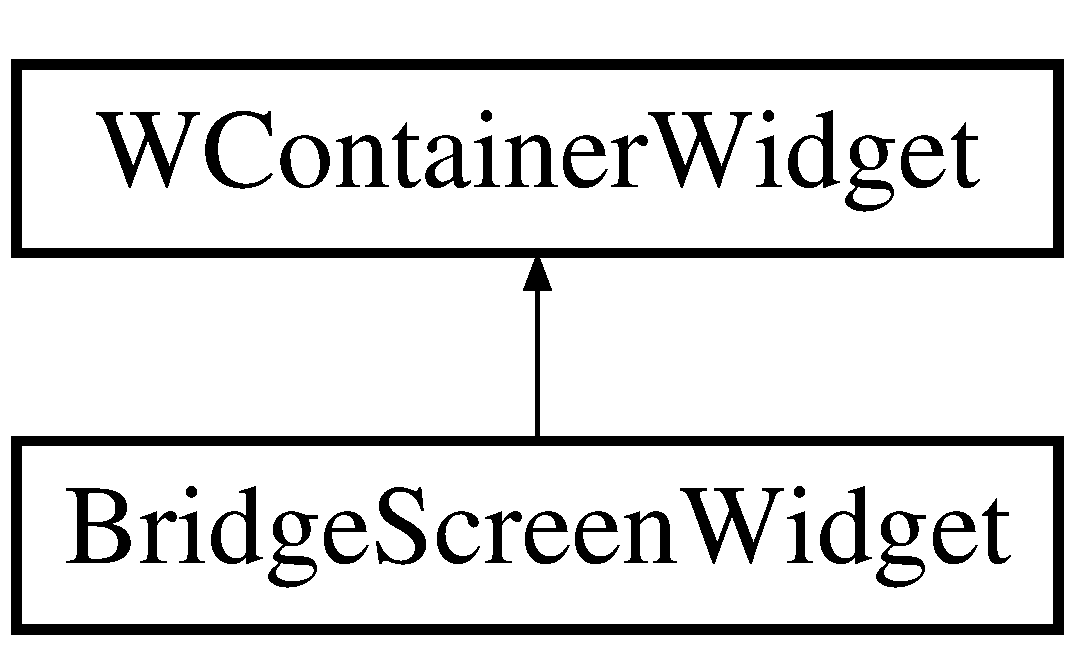
\includegraphics[height=2.000000cm]{classBridgeScreenWidget}
\end{center}
\end{figure}
\subsection*{Public Member Functions}
\begin{DoxyCompactItemize}
\item 
\hyperlink{classBridgeScreenWidget_a17d86f1985d1ec0efa19a236d062f754}{Bridge\+Screen\+Widget} (Wt\+::\+W\+Container\+Widget $\ast$parent=0, \hyperlink{classAccount}{Account} $\ast$account=0, \hyperlink{classWelcomeScreen}{Welcome\+Screen} $\ast$main=0)
\begin{DoxyCompactList}\small\item\em \hyperlink{classBridge}{Bridge} Screen Widget constructor. \end{DoxyCompactList}\item 
void \hyperlink{classBridgeScreenWidget_ad04066096ae05d0c96045d3e13c1fd14}{update} ()
\begin{DoxyCompactList}\small\item\em Update function, clears the widget and re-\/populates with elements of the bridge screen. \end{DoxyCompactList}\end{DoxyCompactItemize}
\subsection*{Private Member Functions}
\begin{DoxyCompactItemize}
\item 
void \hyperlink{classBridgeScreenWidget_a7258758ac7316e501053374af067df14}{update\+Bridge\+Table} ()
\begin{DoxyCompactList}\small\item\em Generates list of Bridges connected to user account. \end{DoxyCompactList}\item 
void \hyperlink{classBridgeScreenWidget_af1e58db73b4940c156274e748e39b8d8}{register\+Bridge} ()
\begin{DoxyCompactList}\small\item\em Function called when Register \hyperlink{classBridge}{Bridge} button is pressed to test a connection to the provided U\+RL. \end{DoxyCompactList}\item 
void \hyperlink{classBridgeScreenWidget_ab146eb3da0d286a3a697fa6ce7147a28}{register\+Bridge\+Http} (boost\+::system\+::error\+\_\+code err, const Wt\+::\+Http\+::\+Message \&response)
\begin{DoxyCompactList}\small\item\em Function to handle the Http response generated by the Wt Http Client object in the \hyperlink{classBridgeScreenWidget_af1e58db73b4940c156274e748e39b8d8}{register\+Bridge()} function. \end{DoxyCompactList}\item 
void \hyperlink{classBridgeScreenWidget_af1bbb293408fa78fb5812e079cb1ee69}{view\+Bridge} (int pos)
\begin{DoxyCompactList}\small\item\em View the specific \hyperlink{classBridge}{Bridge} connected to user account. Returns status message from Http method if the \hyperlink{classBridge}{Bridge} is unreachable. \end{DoxyCompactList}\item 
void \hyperlink{classBridgeScreenWidget_a6a21f3a059a4675d353f3d25cca72562}{view\+Bridge\+Http} (int pos, boost\+::system\+::error\+\_\+code err, const Wt\+::\+Http\+::\+Message \&response)
\begin{DoxyCompactList}\small\item\em Function to handle the Http response generated by the Wt Http Client object in the \hyperlink{classBridgeScreenWidget_af1bbb293408fa78fb5812e079cb1ee69}{view\+Bridge()} function. \end{DoxyCompactList}\item 
void \hyperlink{classBridgeScreenWidget_a01197d21b3419e805f6b80730968125c}{edit\+Bridge} (int pos)
\begin{DoxyCompactList}\small\item\em Opens a W\+Dialog box to edit info for specified \hyperlink{classBridge}{Bridge}. \end{DoxyCompactList}\item 
void \hyperlink{classBridgeScreenWidget_ab9e34361cb5786cfdb3cdbf1cabd2373}{share\+Bridge\+Dialog} (int pos)
\begin{DoxyCompactList}\small\item\em Opens a W\+Dialog box to share specified \hyperlink{classBridge}{Bridge}. \end{DoxyCompactList}\item 
void \hyperlink{classBridgeScreenWidget_aca0e0c21ce0493f04df0dfffc961c0c0}{share\+Bridge} (int pos)
\begin{DoxyCompactList}\small\item\em share specific \hyperlink{classBridge}{Bridge} connected to user account to another user account. Returns status message from Http method if the \hyperlink{classBridge}{Bridge} is unreachable. \end{DoxyCompactList}\item 
void \hyperlink{classBridgeScreenWidget_a0a0aee92cd4bb6f46bca10c04ea06436}{update\+Bridge} (int pos)
\begin{DoxyCompactList}\small\item\em Edit specific \hyperlink{classBridge}{Bridge} connected to user account. Returns status message from Http method if the \hyperlink{classBridge}{Bridge} is unreachable. \end{DoxyCompactList}\item 
void \hyperlink{classBridgeScreenWidget_a29b1325ddad5cca2e6115aca2d015858}{update\+Bridge\+Http} (int pos, boost\+::system\+::error\+\_\+code err, const Wt\+::\+Http\+::\+Message \&response)
\begin{DoxyCompactList}\small\item\em Function to handle the Http response generated by the Wt Http Client object in the \hyperlink{classBridgeScreenWidget_a0a0aee92cd4bb6f46bca10c04ea06436}{update\+Bridge()} function. \end{DoxyCompactList}\item 
void \hyperlink{classBridgeScreenWidget_aaec5d0b09c39ef00ba0c0ab89948106d}{remove\+Bridge} (int pos)
\begin{DoxyCompactList}\small\item\em Removes a \hyperlink{classBridge}{Bridge} from user account. \end{DoxyCompactList}\end{DoxyCompactItemize}
\subsection*{Private Attributes}
\begin{DoxyCompactItemize}
\item 
\hyperlink{classWelcomeScreen}{Welcome\+Screen} $\ast$ {\bfseries parent\+\_\+}\hypertarget{classBridgeScreenWidget_af8f47df9574c3ec047c5866a827d19f6}{}\label{classBridgeScreenWidget_af8f47df9574c3ec047c5866a827d19f6}

\item 
\hyperlink{classAccount}{Account} $\ast$ {\bfseries account\+\_\+}\hypertarget{classBridgeScreenWidget_a177d83a224d50ae375848c0f9c57a357}{}\label{classBridgeScreenWidget_a177d83a224d50ae375848c0f9c57a357}

\item 
Wt\+::\+W\+Line\+Edit $\ast$ {\bfseries bridgename\+\_\+}\hypertarget{classBridgeScreenWidget_a21259cc0247d029758cbc35c5185299c}{}\label{classBridgeScreenWidget_a21259cc0247d029758cbc35c5185299c}

\item 
Wt\+::\+W\+Line\+Edit $\ast$ {\bfseries location\+\_\+}\hypertarget{classBridgeScreenWidget_a73d49d42d86f7f7c28c0ed5f818a616f}{}\label{classBridgeScreenWidget_a73d49d42d86f7f7c28c0ed5f818a616f}

\item 
Wt\+::\+W\+Line\+Edit $\ast$ {\bfseries ip\+\_\+}\hypertarget{classBridgeScreenWidget_aa6027b21f535e185d7aa1fd70810ebec}{}\label{classBridgeScreenWidget_aa6027b21f535e185d7aa1fd70810ebec}

\item 
Wt\+::\+W\+Line\+Edit $\ast$ {\bfseries port\+\_\+}\hypertarget{classBridgeScreenWidget_acc1555746193acdaa857f9560decd6f4}{}\label{classBridgeScreenWidget_acc1555746193acdaa857f9560decd6f4}

\item 
Wt\+::\+W\+Line\+Edit $\ast$ {\bfseries username\+\_\+}\hypertarget{classBridgeScreenWidget_adca68cfe5788f3901411ddac62a323e2}{}\label{classBridgeScreenWidget_adca68cfe5788f3901411ddac62a323e2}

\item 
W\+Table $\ast$ {\bfseries bridge\+Table\+\_\+}\hypertarget{classBridgeScreenWidget_ad67fd68129ae865b0f384410d4d1d257}{}\label{classBridgeScreenWidget_ad67fd68129ae865b0f384410d4d1d257}

\item 
Wt\+::\+W\+Text $\ast$ {\bfseries status\+Message\+\_\+}\hypertarget{classBridgeScreenWidget_af9bbdeea8e3bb29173622b3db3543f94}{}\label{classBridgeScreenWidget_af9bbdeea8e3bb29173622b3db3543f94}

\item 
Wt\+::\+W\+Push\+Button $\ast$ {\bfseries register\+Bridge\+Button\+\_\+}\hypertarget{classBridgeScreenWidget_a8ac40e8c174234367d0adadfa6e1ba9a}{}\label{classBridgeScreenWidget_a8ac40e8c174234367d0adadfa6e1ba9a}

\item 
Wt\+::\+W\+Reg\+Exp\+Validator $\ast$ {\bfseries ip\+Validator\+\_\+}\hypertarget{classBridgeScreenWidget_afe0cbff70d477954e2db43a1d10f5d32}{}\label{classBridgeScreenWidget_afe0cbff70d477954e2db43a1d10f5d32}

\item 
Wt\+::\+W\+Reg\+Exp\+Validator $\ast$ {\bfseries string\+Validator\+\_\+}\hypertarget{classBridgeScreenWidget_a8a8a68b392c57c3d773846d6d92ddd5f}{}\label{classBridgeScreenWidget_a8a8a68b392c57c3d773846d6d92ddd5f}

\item 
Wt\+::\+W\+Reg\+Exp\+Validator $\ast$ {\bfseries userid\+Validator\+\_\+}\hypertarget{classBridgeScreenWidget_a20027cd1b92695283dcb28912fe8cff9}{}\label{classBridgeScreenWidget_a20027cd1b92695283dcb28912fe8cff9}

\item 
Wt\+::\+W\+Int\+Validator $\ast$ {\bfseries port\+Validator\+\_\+}\hypertarget{classBridgeScreenWidget_ab6393fbeb84cb9d673ded2e28f9a08db}{}\label{classBridgeScreenWidget_ab6393fbeb84cb9d673ded2e28f9a08db}

\item 
Wt\+::\+W\+Dialog $\ast$ {\bfseries bridge\+Edit\+Dialog\+\_\+}\hypertarget{classBridgeScreenWidget_ac9251092c8dc04ac714b3e60d386ba70}{}\label{classBridgeScreenWidget_ac9251092c8dc04ac714b3e60d386ba70}

\item 
Wt\+::\+W\+Line\+Edit $\ast$ {\bfseries bridge\+Edit\+Name\+\_\+}\hypertarget{classBridgeScreenWidget_ace3c923b82ed9010a29d1905c332cac9}{}\label{classBridgeScreenWidget_ace3c923b82ed9010a29d1905c332cac9}

\item 
Wt\+::\+W\+Line\+Edit $\ast$ {\bfseries bridge\+Edit\+Location\+\_\+}\hypertarget{classBridgeScreenWidget_a53ee53a40c39c1800730fa13bf097713}{}\label{classBridgeScreenWidget_a53ee53a40c39c1800730fa13bf097713}

\item 
Wt\+::\+W\+Line\+Edit $\ast$ {\bfseries bridge\+Edit\+I\+P\+\_\+}\hypertarget{classBridgeScreenWidget_a75e3284d265f702ce9ae8866890f1b9c}{}\label{classBridgeScreenWidget_a75e3284d265f702ce9ae8866890f1b9c}

\item 
Wt\+::\+W\+Line\+Edit $\ast$ {\bfseries bridge\+Edit\+Port\+\_\+}\hypertarget{classBridgeScreenWidget_ae770a21f977251199e28bef894d18fe4}{}\label{classBridgeScreenWidget_ae770a21f977251199e28bef894d18fe4}

\item 
Wt\+::\+W\+Line\+Edit $\ast$ {\bfseries bridge\+Edit\+Username\+\_\+}\hypertarget{classBridgeScreenWidget_a2dddf96c279cf0c2bb97618fc9a4a257}{}\label{classBridgeScreenWidget_a2dddf96c279cf0c2bb97618fc9a4a257}

\item 
Wt\+::\+W\+Dialog $\ast$ {\bfseries bridge\+Share\+Dialog\+\_\+}\hypertarget{classBridgeScreenWidget_a5aba3d68af7a344f3577936a51692b48}{}\label{classBridgeScreenWidget_a5aba3d68af7a344f3577936a51692b48}

\item 
Wt\+::\+W\+Line\+Edit $\ast$ {\bfseries bridge\+Share\+Userid\+\_\+}\hypertarget{classBridgeScreenWidget_ad00207919171e486b77e70a465cfc529}{}\label{classBridgeScreenWidget_ad00207919171e486b77e70a465cfc529}

\item 
\hyperlink{classBridge}{Bridge} $\ast$ {\bfseries bridge\+\_\+}\hypertarget{classBridgeScreenWidget_a95be4ea490f2e043cd3ff36cd7d6a73b}{}\label{classBridgeScreenWidget_a95be4ea490f2e043cd3ff36cd7d6a73b}

\end{DoxyCompactItemize}


\subsection{Constructor \& Destructor Documentation}
\index{Bridge\+Screen\+Widget@{Bridge\+Screen\+Widget}!Bridge\+Screen\+Widget@{Bridge\+Screen\+Widget}}
\index{Bridge\+Screen\+Widget@{Bridge\+Screen\+Widget}!Bridge\+Screen\+Widget@{Bridge\+Screen\+Widget}}
\subsubsection[{\texorpdfstring{Bridge\+Screen\+Widget(\+Wt\+::\+W\+Container\+Widget $\ast$parent=0, Account $\ast$account=0, Welcome\+Screen $\ast$main=0)}{BridgeScreenWidget(Wt::WContainerWidget *parent=0, Account *account=0, WelcomeScreen *main=0)}}]{\setlength{\rightskip}{0pt plus 5cm}Bridge\+Screen\+Widget\+::\+Bridge\+Screen\+Widget (
\begin{DoxyParamCaption}
\item[{Wt\+::\+W\+Container\+Widget $\ast$}]{parent = {\ttfamily 0}, }
\item[{{\bf Account} $\ast$}]{account = {\ttfamily 0}, }
\item[{{\bf Welcome\+Screen} $\ast$}]{main = {\ttfamily 0}}
\end{DoxyParamCaption}
)}\hypertarget{classBridgeScreenWidget_a17d86f1985d1ec0efa19a236d062f754}{}\label{classBridgeScreenWidget_a17d86f1985d1ec0efa19a236d062f754}


\hyperlink{classBridge}{Bridge} Screen Widget constructor. 


\begin{DoxyParams}{Parameters}
{\em $\ast$parent} & is a pointer the the containerwidget that stores this widget \\
\hline
{\em $\ast$account} & is a pointer to the user account object \\
\hline
{\em $\ast$main} & is a pointer to the app\textquotesingle{}s welcome screen \\
\hline
\end{DoxyParams}


\subsection{Member Function Documentation}
\index{Bridge\+Screen\+Widget@{Bridge\+Screen\+Widget}!edit\+Bridge@{edit\+Bridge}}
\index{edit\+Bridge@{edit\+Bridge}!Bridge\+Screen\+Widget@{Bridge\+Screen\+Widget}}
\subsubsection[{\texorpdfstring{edit\+Bridge(int pos)}{editBridge(int pos)}}]{\setlength{\rightskip}{0pt plus 5cm}void Bridge\+Screen\+Widget\+::edit\+Bridge (
\begin{DoxyParamCaption}
\item[{int}]{pos}
\end{DoxyParamCaption}
)\hspace{0.3cm}{\ttfamily [private]}}\hypertarget{classBridgeScreenWidget_a01197d21b3419e805f6b80730968125c}{}\label{classBridgeScreenWidget_a01197d21b3419e805f6b80730968125c}


Opens a W\+Dialog box to edit info for specified \hyperlink{classBridge}{Bridge}. 


\begin{DoxyParams}{Parameters}
{\em pos} & the position of the \hyperlink{classBridge}{Bridge} in user account vector to view\\
\hline
\end{DoxyParams}
\begin{DoxyReturn}{Returns}
void 
\end{DoxyReturn}
\index{Bridge\+Screen\+Widget@{Bridge\+Screen\+Widget}!register\+Bridge@{register\+Bridge}}
\index{register\+Bridge@{register\+Bridge}!Bridge\+Screen\+Widget@{Bridge\+Screen\+Widget}}
\subsubsection[{\texorpdfstring{register\+Bridge()}{registerBridge()}}]{\setlength{\rightskip}{0pt plus 5cm}void Bridge\+Screen\+Widget\+::register\+Bridge (
\begin{DoxyParamCaption}
{}
\end{DoxyParamCaption}
)\hspace{0.3cm}{\ttfamily [private]}}\hypertarget{classBridgeScreenWidget_af1e58db73b4940c156274e748e39b8d8}{}\label{classBridgeScreenWidget_af1e58db73b4940c156274e748e39b8d8}


Function called when Register \hyperlink{classBridge}{Bridge} button is pressed to test a connection to the provided U\+RL. 

\begin{DoxyReturn}{Returns}
void 
\end{DoxyReturn}
\index{Bridge\+Screen\+Widget@{Bridge\+Screen\+Widget}!register\+Bridge\+Http@{register\+Bridge\+Http}}
\index{register\+Bridge\+Http@{register\+Bridge\+Http}!Bridge\+Screen\+Widget@{Bridge\+Screen\+Widget}}
\subsubsection[{\texorpdfstring{register\+Bridge\+Http(boost\+::system\+::error\+\_\+code err, const Wt\+::\+Http\+::\+Message \&response)}{registerBridgeHttp(boost::system::error_code err, const Wt::Http::Message &response)}}]{\setlength{\rightskip}{0pt plus 5cm}void Bridge\+Screen\+Widget\+::register\+Bridge\+Http (
\begin{DoxyParamCaption}
\item[{boost\+::system\+::error\+\_\+code}]{err, }
\item[{const Wt\+::\+Http\+::\+Message \&}]{response}
\end{DoxyParamCaption}
)\hspace{0.3cm}{\ttfamily [private]}}\hypertarget{classBridgeScreenWidget_ab146eb3da0d286a3a697fa6ce7147a28}{}\label{classBridgeScreenWidget_ab146eb3da0d286a3a697fa6ce7147a28}


Function to handle the Http response generated by the Wt Http Client object in the \hyperlink{classBridgeScreenWidget_af1e58db73b4940c156274e748e39b8d8}{register\+Bridge()} function. 


\begin{DoxyParams}{Parameters}
{\em $\ast$err} & stores the error code generated by an Http request, null if request was successful \\
\hline
{\em \&response} & stores the response message generated by the Http request\\
\hline
\end{DoxyParams}
\begin{DoxyReturn}{Returns}
void 
\end{DoxyReturn}
\index{Bridge\+Screen\+Widget@{Bridge\+Screen\+Widget}!remove\+Bridge@{remove\+Bridge}}
\index{remove\+Bridge@{remove\+Bridge}!Bridge\+Screen\+Widget@{Bridge\+Screen\+Widget}}
\subsubsection[{\texorpdfstring{remove\+Bridge(int pos)}{removeBridge(int pos)}}]{\setlength{\rightskip}{0pt plus 5cm}void Bridge\+Screen\+Widget\+::remove\+Bridge (
\begin{DoxyParamCaption}
\item[{int}]{pos}
\end{DoxyParamCaption}
)\hspace{0.3cm}{\ttfamily [private]}}\hypertarget{classBridgeScreenWidget_aaec5d0b09c39ef00ba0c0ab89948106d}{}\label{classBridgeScreenWidget_aaec5d0b09c39ef00ba0c0ab89948106d}


Removes a \hyperlink{classBridge}{Bridge} from user account. 


\begin{DoxyParams}{Parameters}
{\em pos} & the position of the \hyperlink{classBridge}{Bridge} in the vector to remove\\
\hline
\end{DoxyParams}
\begin{DoxyReturn}{Returns}
void 
\end{DoxyReturn}
\index{Bridge\+Screen\+Widget@{Bridge\+Screen\+Widget}!share\+Bridge@{share\+Bridge}}
\index{share\+Bridge@{share\+Bridge}!Bridge\+Screen\+Widget@{Bridge\+Screen\+Widget}}
\subsubsection[{\texorpdfstring{share\+Bridge(int pos)}{shareBridge(int pos)}}]{\setlength{\rightskip}{0pt plus 5cm}void Bridge\+Screen\+Widget\+::share\+Bridge (
\begin{DoxyParamCaption}
\item[{int}]{pos}
\end{DoxyParamCaption}
)\hspace{0.3cm}{\ttfamily [private]}}\hypertarget{classBridgeScreenWidget_aca0e0c21ce0493f04df0dfffc961c0c0}{}\label{classBridgeScreenWidget_aca0e0c21ce0493f04df0dfffc961c0c0}


share specific \hyperlink{classBridge}{Bridge} connected to user account to another user account. Returns status message from Http method if the \hyperlink{classBridge}{Bridge} is unreachable. 


\begin{DoxyParams}{Parameters}
{\em pos} & the position of the \hyperlink{classBridge}{Bridge} in user account vector to update\\
\hline
\end{DoxyParams}
\begin{DoxyReturn}{Returns}
void 
\end{DoxyReturn}
\index{Bridge\+Screen\+Widget@{Bridge\+Screen\+Widget}!share\+Bridge\+Dialog@{share\+Bridge\+Dialog}}
\index{share\+Bridge\+Dialog@{share\+Bridge\+Dialog}!Bridge\+Screen\+Widget@{Bridge\+Screen\+Widget}}
\subsubsection[{\texorpdfstring{share\+Bridge\+Dialog(int pos)}{shareBridgeDialog(int pos)}}]{\setlength{\rightskip}{0pt plus 5cm}void Bridge\+Screen\+Widget\+::share\+Bridge\+Dialog (
\begin{DoxyParamCaption}
\item[{int}]{pos}
\end{DoxyParamCaption}
)\hspace{0.3cm}{\ttfamily [private]}}\hypertarget{classBridgeScreenWidget_ab9e34361cb5786cfdb3cdbf1cabd2373}{}\label{classBridgeScreenWidget_ab9e34361cb5786cfdb3cdbf1cabd2373}


Opens a W\+Dialog box to share specified \hyperlink{classBridge}{Bridge}. 


\begin{DoxyParams}{Parameters}
{\em pos} & the position of the \hyperlink{classBridge}{Bridge} in user account vector to view\\
\hline
\end{DoxyParams}
\begin{DoxyReturn}{Returns}
void 
\end{DoxyReturn}
\index{Bridge\+Screen\+Widget@{Bridge\+Screen\+Widget}!update@{update}}
\index{update@{update}!Bridge\+Screen\+Widget@{Bridge\+Screen\+Widget}}
\subsubsection[{\texorpdfstring{update()}{update()}}]{\setlength{\rightskip}{0pt plus 5cm}void Bridge\+Screen\+Widget\+::update (
\begin{DoxyParamCaption}
{}
\end{DoxyParamCaption}
)}\hypertarget{classBridgeScreenWidget_ad04066096ae05d0c96045d3e13c1fd14}{}\label{classBridgeScreenWidget_ad04066096ae05d0c96045d3e13c1fd14}


Update function, clears the widget and re-\/populates with elements of the bridge screen. 

\begin{DoxyReturn}{Returns}
void 
\end{DoxyReturn}
\index{Bridge\+Screen\+Widget@{Bridge\+Screen\+Widget}!update\+Bridge@{update\+Bridge}}
\index{update\+Bridge@{update\+Bridge}!Bridge\+Screen\+Widget@{Bridge\+Screen\+Widget}}
\subsubsection[{\texorpdfstring{update\+Bridge(int pos)}{updateBridge(int pos)}}]{\setlength{\rightskip}{0pt plus 5cm}void Bridge\+Screen\+Widget\+::update\+Bridge (
\begin{DoxyParamCaption}
\item[{int}]{pos}
\end{DoxyParamCaption}
)\hspace{0.3cm}{\ttfamily [private]}}\hypertarget{classBridgeScreenWidget_a0a0aee92cd4bb6f46bca10c04ea06436}{}\label{classBridgeScreenWidget_a0a0aee92cd4bb6f46bca10c04ea06436}


Edit specific \hyperlink{classBridge}{Bridge} connected to user account. Returns status message from Http method if the \hyperlink{classBridge}{Bridge} is unreachable. 


\begin{DoxyParams}{Parameters}
{\em pos} & the position of the \hyperlink{classBridge}{Bridge} in user account vector to update\\
\hline
\end{DoxyParams}
\begin{DoxyReturn}{Returns}
void 
\end{DoxyReturn}
\index{Bridge\+Screen\+Widget@{Bridge\+Screen\+Widget}!update\+Bridge\+Http@{update\+Bridge\+Http}}
\index{update\+Bridge\+Http@{update\+Bridge\+Http}!Bridge\+Screen\+Widget@{Bridge\+Screen\+Widget}}
\subsubsection[{\texorpdfstring{update\+Bridge\+Http(int pos, boost\+::system\+::error\+\_\+code err, const Wt\+::\+Http\+::\+Message \&response)}{updateBridgeHttp(int pos, boost::system::error_code err, const Wt::Http::Message &response)}}]{\setlength{\rightskip}{0pt plus 5cm}void Bridge\+Screen\+Widget\+::update\+Bridge\+Http (
\begin{DoxyParamCaption}
\item[{int}]{pos, }
\item[{boost\+::system\+::error\+\_\+code}]{err, }
\item[{const Wt\+::\+Http\+::\+Message \&}]{response}
\end{DoxyParamCaption}
)\hspace{0.3cm}{\ttfamily [private]}}\hypertarget{classBridgeScreenWidget_a29b1325ddad5cca2e6115aca2d015858}{}\label{classBridgeScreenWidget_a29b1325ddad5cca2e6115aca2d015858}


Function to handle the Http response generated by the Wt Http Client object in the \hyperlink{classBridgeScreenWidget_a0a0aee92cd4bb6f46bca10c04ea06436}{update\+Bridge()} function. 


\begin{DoxyParams}{Parameters}
{\em pos} & the position of the \hyperlink{classBridge}{Bridge} being accessed \\
\hline
{\em $\ast$err} & stores the error code generated by an Http request, null if request was successful \\
\hline
{\em \&response} & stores the response message generated by the Http request\\
\hline
\end{DoxyParams}
\begin{DoxyReturn}{Returns}
void 
\end{DoxyReturn}
\index{Bridge\+Screen\+Widget@{Bridge\+Screen\+Widget}!update\+Bridge\+Table@{update\+Bridge\+Table}}
\index{update\+Bridge\+Table@{update\+Bridge\+Table}!Bridge\+Screen\+Widget@{Bridge\+Screen\+Widget}}
\subsubsection[{\texorpdfstring{update\+Bridge\+Table()}{updateBridgeTable()}}]{\setlength{\rightskip}{0pt plus 5cm}void Bridge\+Screen\+Widget\+::update\+Bridge\+Table (
\begin{DoxyParamCaption}
{}
\end{DoxyParamCaption}
)\hspace{0.3cm}{\ttfamily [private]}}\hypertarget{classBridgeScreenWidget_a7258758ac7316e501053374af067df14}{}\label{classBridgeScreenWidget_a7258758ac7316e501053374af067df14}


Generates list of Bridges connected to user account. 

\begin{DoxyReturn}{Returns}
void 
\end{DoxyReturn}
\index{Bridge\+Screen\+Widget@{Bridge\+Screen\+Widget}!view\+Bridge@{view\+Bridge}}
\index{view\+Bridge@{view\+Bridge}!Bridge\+Screen\+Widget@{Bridge\+Screen\+Widget}}
\subsubsection[{\texorpdfstring{view\+Bridge(int pos)}{viewBridge(int pos)}}]{\setlength{\rightskip}{0pt plus 5cm}void Bridge\+Screen\+Widget\+::view\+Bridge (
\begin{DoxyParamCaption}
\item[{int}]{pos}
\end{DoxyParamCaption}
)\hspace{0.3cm}{\ttfamily [private]}}\hypertarget{classBridgeScreenWidget_af1bbb293408fa78fb5812e079cb1ee69}{}\label{classBridgeScreenWidget_af1bbb293408fa78fb5812e079cb1ee69}


View the specific \hyperlink{classBridge}{Bridge} connected to user account. Returns status message from Http method if the \hyperlink{classBridge}{Bridge} is unreachable. 


\begin{DoxyParams}{Parameters}
{\em pos} & the position of the \hyperlink{classBridge}{Bridge} in user account vector to view\\
\hline
\end{DoxyParams}
\begin{DoxyReturn}{Returns}
void 
\end{DoxyReturn}
\index{Bridge\+Screen\+Widget@{Bridge\+Screen\+Widget}!view\+Bridge\+Http@{view\+Bridge\+Http}}
\index{view\+Bridge\+Http@{view\+Bridge\+Http}!Bridge\+Screen\+Widget@{Bridge\+Screen\+Widget}}
\subsubsection[{\texorpdfstring{view\+Bridge\+Http(int pos, boost\+::system\+::error\+\_\+code err, const Wt\+::\+Http\+::\+Message \&response)}{viewBridgeHttp(int pos, boost::system::error_code err, const Wt::Http::Message &response)}}]{\setlength{\rightskip}{0pt plus 5cm}void Bridge\+Screen\+Widget\+::view\+Bridge\+Http (
\begin{DoxyParamCaption}
\item[{int}]{pos, }
\item[{boost\+::system\+::error\+\_\+code}]{err, }
\item[{const Wt\+::\+Http\+::\+Message \&}]{response}
\end{DoxyParamCaption}
)\hspace{0.3cm}{\ttfamily [private]}}\hypertarget{classBridgeScreenWidget_a6a21f3a059a4675d353f3d25cca72562}{}\label{classBridgeScreenWidget_a6a21f3a059a4675d353f3d25cca72562}


Function to handle the Http response generated by the Wt Http Client object in the \hyperlink{classBridgeScreenWidget_af1bbb293408fa78fb5812e079cb1ee69}{view\+Bridge()} function. 


\begin{DoxyParams}{Parameters}
{\em pos} & the position of the \hyperlink{classBridge}{Bridge} being accessed \\
\hline
{\em $\ast$err} & stores the error code generated by an Http request, null if request was successful \\
\hline
{\em \&response} & stores the response message generated by the Http request\\
\hline
\end{DoxyParams}
\begin{DoxyReturn}{Returns}
void 
\end{DoxyReturn}


The documentation for this class was generated from the following files\+:\begin{DoxyCompactItemize}
\item 
include/Bridge\+Screen\+Widget.\+h\item 
src/\hyperlink{BridgeScreenWidget_8cpp}{Bridge\+Screen\+Widget.\+cpp}\end{DoxyCompactItemize}

\hypertarget{classColourConvert}{}\section{Colour\+Convert Class Reference}
\label{classColourConvert}\index{Colour\+Convert@{Colour\+Convert}}
\subsection*{Static Public Member Functions}
\begin{DoxyCompactItemize}
\item 
static struct \hyperlink{structxy}{xy} $\ast$ \hyperlink{classColourConvert_a16ccfb2d7b81c54e46f9a3b827b7c8c2}{rgb2xy} (float red, float green, float blue)
\begin{DoxyCompactList}\small\item\em R\+GB to XY converter. \end{DoxyCompactList}\item 
static struct \hyperlink{structrgb}{rgb} $\ast$ \hyperlink{classColourConvert_a9540a0b33ca2703355f9dd0629fc1cd2}{xy2rgb} (float x, float y, float brightness)
\begin{DoxyCompactList}\small\item\em XY to R\+GB converter. \end{DoxyCompactList}\item 
static struct \hyperlink{structrgb}{rgb} $\ast$ \hyperlink{classColourConvert_a27e116384a459a5e2622ee37ab72103d}{hsv2rgb} (float hue, float sat, float bri)
\begin{DoxyCompactList}\small\item\em Hue Sat Bri to R\+GB converter. \end{DoxyCompactList}\end{DoxyCompactItemize}


\subsection{Member Function Documentation}
\index{Colour\+Convert@{Colour\+Convert}!hsv2rgb@{hsv2rgb}}
\index{hsv2rgb@{hsv2rgb}!Colour\+Convert@{Colour\+Convert}}
\subsubsection[{\texorpdfstring{hsv2rgb(float hue, float sat, float bri)}{hsv2rgb(float hue, float sat, float bri)}}]{\setlength{\rightskip}{0pt plus 5cm}struct {\bf rgb} $\ast$ Colour\+Convert\+::hsv2rgb (
\begin{DoxyParamCaption}
\item[{float}]{hue, }
\item[{float}]{sat, }
\item[{float}]{bri}
\end{DoxyParamCaption}
)\hspace{0.3cm}{\ttfamily [static]}}\hypertarget{classColourConvert_a27e116384a459a5e2622ee37ab72103d}{}\label{classColourConvert_a27e116384a459a5e2622ee37ab72103d}


Hue Sat Bri to R\+GB converter. 


\begin{DoxyParams}{Parameters}
{\em hue} & is the Hue component of the colour \\
\hline
{\em sat} & is the Sat component of the colour \\
\hline
{\em bri} & is the Brightness value of the light\\
\hline
\end{DoxyParams}
\begin{DoxyReturn}{Returns}
struct rgb containing R\+GB value representation of parameters 
\end{DoxyReturn}
\index{Colour\+Convert@{Colour\+Convert}!rgb2xy@{rgb2xy}}
\index{rgb2xy@{rgb2xy}!Colour\+Convert@{Colour\+Convert}}
\subsubsection[{\texorpdfstring{rgb2xy(float red, float green, float blue)}{rgb2xy(float red, float green, float blue)}}]{\setlength{\rightskip}{0pt plus 5cm}struct {\bf xy} $\ast$ Colour\+Convert\+::rgb2xy (
\begin{DoxyParamCaption}
\item[{float}]{r, }
\item[{float}]{g, }
\item[{float}]{b}
\end{DoxyParamCaption}
)\hspace{0.3cm}{\ttfamily [static]}}\hypertarget{classColourConvert_a16ccfb2d7b81c54e46f9a3b827b7c8c2}{}\label{classColourConvert_a16ccfb2d7b81c54e46f9a3b827b7c8c2}


R\+GB to XY converter. 


\begin{DoxyParams}{Parameters}
{\em r} & is the red component of the colour \\
\hline
{\em g} & is the green component of the colour \\
\hline
{\em b} & is the blue component of the colour\\
\hline
\end{DoxyParams}
\begin{DoxyReturn}{Returns}
struct xy containing XY value representation of parameters 
\end{DoxyReturn}
\index{Colour\+Convert@{Colour\+Convert}!xy2rgb@{xy2rgb}}
\index{xy2rgb@{xy2rgb}!Colour\+Convert@{Colour\+Convert}}
\subsubsection[{\texorpdfstring{xy2rgb(float x, float y, float brightness)}{xy2rgb(float x, float y, float brightness)}}]{\setlength{\rightskip}{0pt plus 5cm}struct {\bf rgb} $\ast$ Colour\+Convert\+::xy2rgb (
\begin{DoxyParamCaption}
\item[{float}]{inputX, }
\item[{float}]{inputY, }
\item[{float}]{brightness}
\end{DoxyParamCaption}
)\hspace{0.3cm}{\ttfamily [static]}}\hypertarget{classColourConvert_a9540a0b33ca2703355f9dd0629fc1cd2}{}\label{classColourConvert_a9540a0b33ca2703355f9dd0629fc1cd2}


XY to R\+GB converter. 


\begin{DoxyParams}{Parameters}
{\em inputX} & is the X component of the colour \\
\hline
{\em inputY} & is the Y component of the colour \\
\hline
{\em brightness} & is the brightness value of the light\\
\hline
\end{DoxyParams}
\begin{DoxyReturn}{Returns}
struct rgb containing R\+GB value representation of parameters 
\end{DoxyReturn}


The documentation for this class was generated from the following files\+:\begin{DoxyCompactItemize}
\item 
include/Colour\+Convert.\+h\item 
src/\hyperlink{ColourConvert_8cpp}{Colour\+Convert.\+cpp}\end{DoxyCompactItemize}

\hypertarget{classCreateAccountWidget}{}\section{Create\+Account\+Widget Class Reference}
\label{classCreateAccountWidget}\index{Create\+Account\+Widget@{Create\+Account\+Widget}}
Inheritance diagram for Create\+Account\+Widget\+:\begin{figure}[H]
\begin{center}
\leavevmode
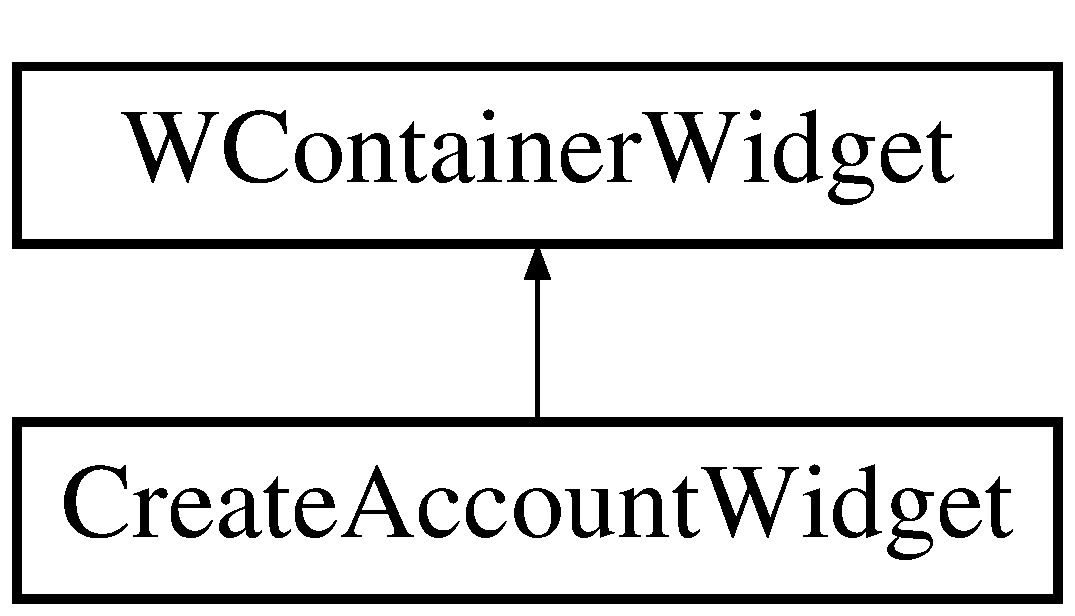
\includegraphics[height=2.000000cm]{classCreateAccountWidget}
\end{center}
\end{figure}
\subsection*{Public Member Functions}
\begin{DoxyCompactItemize}
\item 
\hyperlink{classCreateAccountWidget_afe9017adc69291027c3ebd3f9d448a4c}{Create\+Account\+Widget} (Wt\+::\+W\+Container\+Widget $\ast$parent=0, \hyperlink{classAccount}{Account} $\ast$account=0, \hyperlink{classWelcomeScreen}{Welcome\+Screen} $\ast$main=0)
\begin{DoxyCompactList}\small\item\em Create \hyperlink{classAccount}{Account} Widget constructor. \end{DoxyCompactList}\item 
void \hyperlink{classCreateAccountWidget_a7561efaf407aa50a1dc8fe1c8c099d85}{update} ()
\begin{DoxyCompactList}\small\item\em Update function, clears the widget and re-\/populates with elements of the account creation screen. \end{DoxyCompactList}\end{DoxyCompactItemize}
\subsection*{Private Member Functions}
\begin{DoxyCompactItemize}
\item 
void \hyperlink{classCreateAccountWidget_a07718d46b3c72f481d550d6dfd4290c1}{write\+User\+Info} (std\+::string username, std\+::string password, std\+::string first, std\+::string last)
\begin{DoxyCompactList}\small\item\em write\+Credentials() function, writes an encrypted version of the user\textquotesingle{}s password into username.\+txt \end{DoxyCompactList}\item 
void \hyperlink{classCreateAccountWidget_ae55d754c8605628ff22ae06b6aa6e137}{submit} ()\hypertarget{classCreateAccountWidget_ae55d754c8605628ff22ae06b6aa6e137}{}\label{classCreateAccountWidget_ae55d754c8605628ff22ae06b6aa6e137}

\begin{DoxyCompactList}\small\item\em \hyperlink{classCreateAccountWidget_ae55d754c8605628ff22ae06b6aa6e137}{submit()} function, triggered when user presses create account button, displays any applicable warning messages and/or triggers the account credentials write-\/to-\/file. Finally, it redirects to the login screen. \end{DoxyCompactList}\item 
bool \hyperlink{classCreateAccountWidget_a96b0c9778519832be6406410f0bc3c46}{validate\+Password} ()
\begin{DoxyCompactList}\small\item\em \hyperlink{classCreateAccountWidget_a96b0c9778519832be6406410f0bc3c46}{validate\+Password()} function, confirms the the user\textquotesingle{}s inputted password == inputted confirmed password \end{DoxyCompactList}\item 
bool \hyperlink{classCreateAccountWidget_aa64703ec022e1d643011d1831c5aeae6}{validate\+Input\+Fields} ()
\begin{DoxyCompactList}\small\item\em \hyperlink{classCreateAccountWidget_aa64703ec022e1d643011d1831c5aeae6}{validate\+Input\+Fields()}\+: ensures that username is valid email address and pass is between 6-\/20 chars \end{DoxyCompactList}\item 
bool \hyperlink{classCreateAccountWidget_a485aa50d34319d8eb149d9900f40349f}{check\+New\+Userid} (std\+::string userid)
\begin{DoxyCompactList}\small\item\em check\+New\+User\+Id() function, checks to see if the user\textquotesingle{}s inputted id already exists in the system \end{DoxyCompactList}\end{DoxyCompactItemize}
\subsection*{Private Attributes}
\begin{DoxyCompactItemize}
\item 
Wt\+::\+W\+Line\+Edit $\ast$ {\bfseries username\+\_\+}\hypertarget{classCreateAccountWidget_a6845ece9134008bcd3c32bad833cbc96}{}\label{classCreateAccountWidget_a6845ece9134008bcd3c32bad833cbc96}

\item 
Wt\+::\+W\+Line\+Edit $\ast$ {\bfseries first\+Name\+\_\+}\hypertarget{classCreateAccountWidget_aa4f562845143675adef1764f57e7e3bf}{}\label{classCreateAccountWidget_aa4f562845143675adef1764f57e7e3bf}

\item 
Wt\+::\+W\+Line\+Edit $\ast$ {\bfseries last\+Name\+\_\+}\hypertarget{classCreateAccountWidget_a12fc04957268ff3dcaee4333e96d04fa}{}\label{classCreateAccountWidget_a12fc04957268ff3dcaee4333e96d04fa}

\item 
Wt\+::\+W\+Line\+Edit $\ast$ {\bfseries password\+\_\+}\hypertarget{classCreateAccountWidget_ac3e4d8093f9bfc2ed5f16b7ffa44aeda}{}\label{classCreateAccountWidget_ac3e4d8093f9bfc2ed5f16b7ffa44aeda}

\item 
Wt\+::\+W\+Line\+Edit $\ast$ {\bfseries confirm\+Password\+\_\+}\hypertarget{classCreateAccountWidget_a5af429ae5ba69d0c7b1e1bdb0f7a313e}{}\label{classCreateAccountWidget_a5af429ae5ba69d0c7b1e1bdb0f7a313e}

\item 
Wt\+::\+W\+Push\+Button $\ast$ {\bfseries create\+Account\+Button\+\_\+}\hypertarget{classCreateAccountWidget_a53c12cfed364c82a77ecedd133ccb15e}{}\label{classCreateAccountWidget_a53c12cfed364c82a77ecedd133ccb15e}

\item 
Wt\+::\+W\+Text $\ast$ {\bfseries unsuccessful\+Password\+\_\+}\hypertarget{classCreateAccountWidget_a34cb095702c7060ce35d6e6c5f42bf13}{}\label{classCreateAccountWidget_a34cb095702c7060ce35d6e6c5f42bf13}

\item 
Wt\+::\+W\+Text $\ast$ {\bfseries unsuccessful\+Input\+\_\+}\hypertarget{classCreateAccountWidget_a5b0ef52c652f912ccd9fb4f2dd5d5b94}{}\label{classCreateAccountWidget_a5b0ef52c652f912ccd9fb4f2dd5d5b94}

\item 
Wt\+::\+W\+Text $\ast$ {\bfseries account\+Exists\+\_\+}\hypertarget{classCreateAccountWidget_af8fd1df4209baed3b6037f08c9eb9e30}{}\label{classCreateAccountWidget_af8fd1df4209baed3b6037f08c9eb9e30}

\item 
Wt\+::\+W\+Reg\+Exp\+Validator $\ast$ {\bfseries username\+Validator\+\_\+}\hypertarget{classCreateAccountWidget_ab360ccc42663b0e7f00e728d3974893f}{}\label{classCreateAccountWidget_ab360ccc42663b0e7f00e728d3974893f}

\item 
Wt\+::\+W\+Length\+Validator $\ast$ {\bfseries password\+Length\+Validator\+\_\+}\hypertarget{classCreateAccountWidget_ae4974f817e22c7fd860f7a9f2d491235}{}\label{classCreateAccountWidget_ae4974f817e22c7fd860f7a9f2d491235}

\item 
Wt\+::\+W\+Validator $\ast$ {\bfseries input\+Not\+Empty\+\_\+}\hypertarget{classCreateAccountWidget_a2cb26f1cf86707efc2bcb405ff269482}{}\label{classCreateAccountWidget_a2cb26f1cf86707efc2bcb405ff269482}

\item 
\hyperlink{classWelcomeScreen}{Welcome\+Screen} $\ast$ {\bfseries parent\+\_\+}\hypertarget{classCreateAccountWidget_a420679af87a13ab8957424ef3a2c39d0}{}\label{classCreateAccountWidget_a420679af87a13ab8957424ef3a2c39d0}

\item 
\hyperlink{classAccount}{Account} $\ast$ {\bfseries account\+\_\+}\hypertarget{classCreateAccountWidget_a750c33b1af3f426a0be17dd5b6e89cbf}{}\label{classCreateAccountWidget_a750c33b1af3f426a0be17dd5b6e89cbf}

\end{DoxyCompactItemize}


\subsection{Constructor \& Destructor Documentation}
\index{Create\+Account\+Widget@{Create\+Account\+Widget}!Create\+Account\+Widget@{Create\+Account\+Widget}}
\index{Create\+Account\+Widget@{Create\+Account\+Widget}!Create\+Account\+Widget@{Create\+Account\+Widget}}
\subsubsection[{\texorpdfstring{Create\+Account\+Widget(\+Wt\+::\+W\+Container\+Widget $\ast$parent=0, Account $\ast$account=0, Welcome\+Screen $\ast$main=0)}{CreateAccountWidget(Wt::WContainerWidget *parent=0, Account *account=0, WelcomeScreen *main=0)}}]{\setlength{\rightskip}{0pt plus 5cm}Create\+Account\+Widget\+::\+Create\+Account\+Widget (
\begin{DoxyParamCaption}
\item[{Wt\+::\+W\+Container\+Widget $\ast$}]{parent = {\ttfamily 0}, }
\item[{{\bf Account} $\ast$}]{account = {\ttfamily 0}, }
\item[{{\bf Welcome\+Screen} $\ast$}]{main = {\ttfamily 0}}
\end{DoxyParamCaption}
)}\hypertarget{classCreateAccountWidget_afe9017adc69291027c3ebd3f9d448a4c}{}\label{classCreateAccountWidget_afe9017adc69291027c3ebd3f9d448a4c}


Create \hyperlink{classAccount}{Account} Widget constructor. 


\begin{DoxyParams}{Parameters}
{\em $\ast$parent} & is a pointer the the containerwidget that stores this widget \\
\hline
{\em $\ast$account} & is a pointer to the user account object \\
\hline
{\em $\ast$main} & is a pointer to the app\textquotesingle{}s welcome screen \\
\hline
\end{DoxyParams}


\subsection{Member Function Documentation}
\index{Create\+Account\+Widget@{Create\+Account\+Widget}!check\+New\+Userid@{check\+New\+Userid}}
\index{check\+New\+Userid@{check\+New\+Userid}!Create\+Account\+Widget@{Create\+Account\+Widget}}
\subsubsection[{\texorpdfstring{check\+New\+Userid(std\+::string userid)}{checkNewUserid(std::string userid)}}]{\setlength{\rightskip}{0pt plus 5cm}bool Create\+Account\+Widget\+::check\+New\+Userid (
\begin{DoxyParamCaption}
\item[{std\+::string}]{userid}
\end{DoxyParamCaption}
)\hspace{0.3cm}{\ttfamily [private]}}\hypertarget{classCreateAccountWidget_a485aa50d34319d8eb149d9900f40349f}{}\label{classCreateAccountWidget_a485aa50d34319d8eb149d9900f40349f}


check\+New\+User\+Id() function, checks to see if the user\textquotesingle{}s inputted id already exists in the system 


\begin{DoxyParams}{Parameters}
{\em userid} & is a string representing the user\textquotesingle{}s inputted username \\
\hline
\end{DoxyParams}
\begin{DoxyReturn}{Returns}
bool\+: true if the username is \char`\"{}new\char`\"{} false if already exists 
\end{DoxyReturn}
\index{Create\+Account\+Widget@{Create\+Account\+Widget}!update@{update}}
\index{update@{update}!Create\+Account\+Widget@{Create\+Account\+Widget}}
\subsubsection[{\texorpdfstring{update()}{update()}}]{\setlength{\rightskip}{0pt plus 5cm}void Create\+Account\+Widget\+::update (
\begin{DoxyParamCaption}
{}
\end{DoxyParamCaption}
)}\hypertarget{classCreateAccountWidget_a7561efaf407aa50a1dc8fe1c8c099d85}{}\label{classCreateAccountWidget_a7561efaf407aa50a1dc8fe1c8c099d85}


Update function, clears the widget and re-\/populates with elements of the account creation screen. 

\begin{DoxyReturn}{Returns}
void 
\end{DoxyReturn}
\index{Create\+Account\+Widget@{Create\+Account\+Widget}!validate\+Input\+Fields@{validate\+Input\+Fields}}
\index{validate\+Input\+Fields@{validate\+Input\+Fields}!Create\+Account\+Widget@{Create\+Account\+Widget}}
\subsubsection[{\texorpdfstring{validate\+Input\+Fields()}{validateInputFields()}}]{\setlength{\rightskip}{0pt plus 5cm}bool Create\+Account\+Widget\+::validate\+Input\+Fields (
\begin{DoxyParamCaption}
{}
\end{DoxyParamCaption}
)\hspace{0.3cm}{\ttfamily [private]}}\hypertarget{classCreateAccountWidget_aa64703ec022e1d643011d1831c5aeae6}{}\label{classCreateAccountWidget_aa64703ec022e1d643011d1831c5aeae6}


\hyperlink{classCreateAccountWidget_aa64703ec022e1d643011d1831c5aeae6}{validate\+Input\+Fields()}\+: ensures that username is valid email address and pass is between 6-\/20 chars 

\begin{DoxyReturn}{Returns}
bool true if the input fields are valid, false otherwise 
\end{DoxyReturn}
\index{Create\+Account\+Widget@{Create\+Account\+Widget}!validate\+Password@{validate\+Password}}
\index{validate\+Password@{validate\+Password}!Create\+Account\+Widget@{Create\+Account\+Widget}}
\subsubsection[{\texorpdfstring{validate\+Password()}{validatePassword()}}]{\setlength{\rightskip}{0pt plus 5cm}bool Create\+Account\+Widget\+::validate\+Password (
\begin{DoxyParamCaption}
{}
\end{DoxyParamCaption}
)\hspace{0.3cm}{\ttfamily [private]}}\hypertarget{classCreateAccountWidget_a96b0c9778519832be6406410f0bc3c46}{}\label{classCreateAccountWidget_a96b0c9778519832be6406410f0bc3c46}


\hyperlink{classCreateAccountWidget_a96b0c9778519832be6406410f0bc3c46}{validate\+Password()} function, confirms the the user\textquotesingle{}s inputted password == inputted confirmed password 

\begin{DoxyReturn}{Returns}
bool representing if the passwords are the same or not 
\end{DoxyReturn}
\index{Create\+Account\+Widget@{Create\+Account\+Widget}!write\+User\+Info@{write\+User\+Info}}
\index{write\+User\+Info@{write\+User\+Info}!Create\+Account\+Widget@{Create\+Account\+Widget}}
\subsubsection[{\texorpdfstring{write\+User\+Info(std\+::string username, std\+::string password, std\+::string first, std\+::string last)}{writeUserInfo(std::string username, std::string password, std::string first, std::string last)}}]{\setlength{\rightskip}{0pt plus 5cm}void Create\+Account\+Widget\+::write\+User\+Info (
\begin{DoxyParamCaption}
\item[{std\+::string}]{username, }
\item[{std\+::string}]{password, }
\item[{std\+::string}]{first, }
\item[{std\+::string}]{last}
\end{DoxyParamCaption}
)\hspace{0.3cm}{\ttfamily [private]}}\hypertarget{classCreateAccountWidget_a07718d46b3c72f481d550d6dfd4290c1}{}\label{classCreateAccountWidget_a07718d46b3c72f481d550d6dfd4290c1}


write\+Credentials() function, writes an encrypted version of the user\textquotesingle{}s password into username.\+txt 


\begin{DoxyParams}{Parameters}
{\em username} & is a string representing the user\textquotesingle{}s inputted username \\
\hline
{\em password} & is a string representing the user\textquotesingle{}s inputted password \\
\hline
\end{DoxyParams}


The documentation for this class was generated from the following files\+:\begin{DoxyCompactItemize}
\item 
include/Create\+Account\+Widget.\+h\item 
src/\hyperlink{CreateAccountWidget_8cpp}{Create\+Account\+Widget.\+cpp}\end{DoxyCompactItemize}

\hypertarget{classGroup}{}\section{Group Class Reference}
\label{classGroup}\index{Group@{Group}}
\subsection*{Public Member Functions}
\begin{DoxyCompactItemize}
\item 
\hyperlink{classGroup_a590b0514381a301636531cddb6902342}{Group} (W\+String group\+Num, Json\+::\+Object group\+Data)
\begin{DoxyCompactList}\small\item\em \hyperlink{classGroup}{Group} constructor. \end{DoxyCompactList}\item 
virtual \hyperlink{classGroup_aed00a22ff227ee2657ae44a5cbcedf7c}{$\sim$\+Group} ()\hypertarget{classGroup_aed00a22ff227ee2657ae44a5cbcedf7c}{}\label{classGroup_aed00a22ff227ee2657ae44a5cbcedf7c}

\begin{DoxyCompactList}\small\item\em \hyperlink{classGroup}{Group} destructor. \end{DoxyCompactList}\item 
W\+String {\bfseries get\+Groupnum} ()\hypertarget{classGroup_a1cc1c807eb94eda9f0d7f52f20cc15cf}{}\label{classGroup_a1cc1c807eb94eda9f0d7f52f20cc15cf}

\item 
W\+String {\bfseries get\+Name} ()\hypertarget{classGroup_a7c66c85f9e17f4e2105ccde041e46efa}{}\label{classGroup_a7c66c85f9e17f4e2105ccde041e46efa}

\item 
W\+String {\bfseries get\+Alert} ()\hypertarget{classGroup_ae482bc5d5e63ade2936b36e3b11aec92}{}\label{classGroup_ae482bc5d5e63ade2936b36e3b11aec92}

\item 
int {\bfseries get\+Bri} ()\hypertarget{classGroup_a0e2391c0c8ba8ea362adbfb6c038e5ac}{}\label{classGroup_a0e2391c0c8ba8ea362adbfb6c038e5ac}

\item 
W\+String {\bfseries get\+Colormode} ()\hypertarget{classGroup_a3d05bff68c94f70e2c8720f141ce4d27}{}\label{classGroup_a3d05bff68c94f70e2c8720f141ce4d27}

\item 
int {\bfseries get\+Ct} ()\hypertarget{classGroup_ab89da05f04279379a720c20bdc46c1d3}{}\label{classGroup_ab89da05f04279379a720c20bdc46c1d3}

\item 
W\+String {\bfseries get\+Effect} ()\hypertarget{classGroup_a84f474a3636ee14812beb1ddc8b85b5c}{}\label{classGroup_a84f474a3636ee14812beb1ddc8b85b5c}

\item 
int {\bfseries get\+Hue} ()\hypertarget{classGroup_aa987a57616beb2d9b84bfb61284cb9b3}{}\label{classGroup_aa987a57616beb2d9b84bfb61284cb9b3}

\item 
bool {\bfseries get\+On} ()\hypertarget{classGroup_a130f7ef2d2c34075c84e7957d6f6edd9}{}\label{classGroup_a130f7ef2d2c34075c84e7957d6f6edd9}

\item 
bool {\bfseries get\+Reachable} ()\hypertarget{classGroup_ab6b9ed2d6c905593e8837aea07579f67}{}\label{classGroup_ab6b9ed2d6c905593e8837aea07579f67}

\item 
int {\bfseries get\+Sat} ()\hypertarget{classGroup_ad81eb4c13f966c37be372796acba0e5b}{}\label{classGroup_ad81eb4c13f966c37be372796acba0e5b}

\item 
double {\bfseries getX} ()\hypertarget{classGroup_a374980af9108689f450d06f1075ccac9}{}\label{classGroup_a374980af9108689f450d06f1075ccac9}

\item 
double {\bfseries getY} ()\hypertarget{classGroup_a9359360dae7f2a628ba7ac1733c01491}{}\label{classGroup_a9359360dae7f2a628ba7ac1733c01491}

\item 
vector$<$ W\+String $>$ {\bfseries get\+Lights} ()\hypertarget{classGroup_a6e31fc668177aca4d8ff66446602973e}{}\label{classGroup_a6e31fc668177aca4d8ff66446602973e}

\item 
int {\bfseries get\+Num\+Lights} ()\hypertarget{classGroup_af191d3b61a57aaccc08a11d75c1ece82}{}\label{classGroup_af191d3b61a57aaccc08a11d75c1ece82}

\item 
int {\bfseries get\+Transition} ()\hypertarget{classGroup_a2917e270bec7ce88165828ee0c224a9d}{}\label{classGroup_a2917e270bec7ce88165828ee0c224a9d}

\item 
void {\bfseries set\+Groupnum} (W\+String groupnum)\hypertarget{classGroup_a43e0e9a4a3c3e937132390bcf4a72108}{}\label{classGroup_a43e0e9a4a3c3e937132390bcf4a72108}

\item 
void {\bfseries set\+Name} (W\+String name)\hypertarget{classGroup_a86ac1b935c83378ff37a1a300265bb41}{}\label{classGroup_a86ac1b935c83378ff37a1a300265bb41}

\item 
void {\bfseries set\+Alert} (W\+String alert)\hypertarget{classGroup_afd0b4271a8c296af56ef5d3ff9e80fc9}{}\label{classGroup_afd0b4271a8c296af56ef5d3ff9e80fc9}

\item 
void {\bfseries set\+Bri} (int bri)\hypertarget{classGroup_a57633cb505ad98d535a0b95046cfa981}{}\label{classGroup_a57633cb505ad98d535a0b95046cfa981}

\item 
void {\bfseries set\+Colormode} (W\+String colormode)\hypertarget{classGroup_af2162664d3105d1bfa2a8ec4ff4ea03e}{}\label{classGroup_af2162664d3105d1bfa2a8ec4ff4ea03e}

\item 
void {\bfseries set\+Ct} (int ct)\hypertarget{classGroup_a976125ede586d1add50a81c702d427fd}{}\label{classGroup_a976125ede586d1add50a81c702d427fd}

\item 
void {\bfseries set\+Effect} (W\+String effect)\hypertarget{classGroup_a8022c5f90e7dd47ab1a35f645e93fbf3}{}\label{classGroup_a8022c5f90e7dd47ab1a35f645e93fbf3}

\item 
void {\bfseries set\+Hue} (int hue)\hypertarget{classGroup_a76f7ab63ec6c9df9d05d6c4553320c61}{}\label{classGroup_a76f7ab63ec6c9df9d05d6c4553320c61}

\item 
void {\bfseries set\+On} (bool on)\hypertarget{classGroup_a67bc57e13e2a45b5a20b309fb81e41a2}{}\label{classGroup_a67bc57e13e2a45b5a20b309fb81e41a2}

\item 
void {\bfseries set\+Reachable} (bool reachable)\hypertarget{classGroup_aea6be609d04ab4c57791d3633f903c1d}{}\label{classGroup_aea6be609d04ab4c57791d3633f903c1d}

\item 
void {\bfseries set\+Sat} (int sat)\hypertarget{classGroup_ab10b43f199a15ffb3ba1c47ec83e8150}{}\label{classGroup_ab10b43f199a15ffb3ba1c47ec83e8150}

\item 
void {\bfseries setX} (double x)\hypertarget{classGroup_a637524f920301f7dce2966443d0e5ad4}{}\label{classGroup_a637524f920301f7dce2966443d0e5ad4}

\item 
void {\bfseries setY} (double y)\hypertarget{classGroup_a298e441bf6bf212d04f54a46f0fab171}{}\label{classGroup_a298e441bf6bf212d04f54a46f0fab171}

\item 
void {\bfseries add\+Light} (W\+String light\+Num)\hypertarget{classGroup_ad864c0549ad004c4947aedc65f459c42}{}\label{classGroup_ad864c0549ad004c4947aedc65f459c42}

\item 
void {\bfseries set\+Transition} (int transitiontime)\hypertarget{classGroup_ad584acb8e1e396868870a60740d32bbb}{}\label{classGroup_ad584acb8e1e396868870a60740d32bbb}

\item 
void {\bfseries toggle\+On\+Off} ()\hypertarget{classGroup_a83ce7e4555d5ab4c908a45dbcde4768d}{}\label{classGroup_a83ce7e4555d5ab4c908a45dbcde4768d}

\end{DoxyCompactItemize}
\subsection*{Private Attributes}
\begin{DoxyCompactItemize}
\item 
W\+String {\bfseries groupnum\+\_\+}\hypertarget{classGroup_a69f864c0eaa193a31184fee1eb8d9cc3}{}\label{classGroup_a69f864c0eaa193a31184fee1eb8d9cc3}

\item 
W\+String {\bfseries name\+\_\+}\hypertarget{classGroup_a439a0313617676a27884c5b7ec753cac}{}\label{classGroup_a439a0313617676a27884c5b7ec753cac}

\item 
W\+String {\bfseries alert\+\_\+}\hypertarget{classGroup_a7df4fe1cc462ace7a9ebe195d0219680}{}\label{classGroup_a7df4fe1cc462ace7a9ebe195d0219680}

\item 
int {\bfseries bri\+\_\+}\hypertarget{classGroup_ae1465822502e2e7fceed62c52c560350}{}\label{classGroup_ae1465822502e2e7fceed62c52c560350}

\item 
W\+String {\bfseries colormode\+\_\+}\hypertarget{classGroup_a2385c148bd77147c8f2adb847068daac}{}\label{classGroup_a2385c148bd77147c8f2adb847068daac}

\item 
int {\bfseries ct\+\_\+}\hypertarget{classGroup_a07d2eecc793800eaa227ffef4cf54ce2}{}\label{classGroup_a07d2eecc793800eaa227ffef4cf54ce2}

\item 
W\+String {\bfseries effect\+\_\+}\hypertarget{classGroup_a928932e7cefb654477f549de187f324b}{}\label{classGroup_a928932e7cefb654477f549de187f324b}

\item 
int {\bfseries hue\+\_\+}\hypertarget{classGroup_ac2056dd023283e807ec561fa07f61b1a}{}\label{classGroup_ac2056dd023283e807ec561fa07f61b1a}

\item 
bool {\bfseries on\+\_\+}\hypertarget{classGroup_a33481b9d58a928fea04af9db03c741a7}{}\label{classGroup_a33481b9d58a928fea04af9db03c741a7}

\item 
bool {\bfseries reachable\+\_\+}\hypertarget{classGroup_a3adf9b85e23be6d823031898b9d37104}{}\label{classGroup_a3adf9b85e23be6d823031898b9d37104}

\item 
int {\bfseries sat\+\_\+}\hypertarget{classGroup_a3f102e28fbd254c4c104ff67885a93b1}{}\label{classGroup_a3f102e28fbd254c4c104ff67885a93b1}

\item 
double {\bfseries xy\+\_\+} \mbox{[}2\mbox{]}\hypertarget{classGroup_a93753c40030dd4959cc204a9a95f258f}{}\label{classGroup_a93753c40030dd4959cc204a9a95f258f}

\item 
vector$<$ W\+String $>$ {\bfseries lights\+\_\+}\hypertarget{classGroup_ab1bf4a4040932f79ef88e351b20c28f3}{}\label{classGroup_ab1bf4a4040932f79ef88e351b20c28f3}

\item 
int {\bfseries transitiontime\+\_\+}\hypertarget{classGroup_a27fe62fe9ba809773b2e52a8711f5000}{}\label{classGroup_a27fe62fe9ba809773b2e52a8711f5000}

\end{DoxyCompactItemize}


\subsection{Constructor \& Destructor Documentation}
\index{Group@{Group}!Group@{Group}}
\index{Group@{Group}!Group@{Group}}
\subsubsection[{\texorpdfstring{Group(\+W\+String group\+Num, Json\+::\+Object group\+Data)}{Group(WString groupNum, Json::Object groupData)}}]{\setlength{\rightskip}{0pt plus 5cm}Group\+::\+Group (
\begin{DoxyParamCaption}
\item[{W\+String}]{group\+Num, }
\item[{Json\+::\+Object}]{group\+Data}
\end{DoxyParamCaption}
)}\hypertarget{classGroup_a590b0514381a301636531cddb6902342}{}\label{classGroup_a590b0514381a301636531cddb6902342}


\hyperlink{classGroup}{Group} constructor. 


\begin{DoxyParams}{Parameters}
{\em group\+Num} & the number key for the \hyperlink{classGroup}{Group} in the Hue A\+PI \\
\hline
{\em group\+Data} & the Json object of a \hyperlink{classGroup}{Group} from the Hue A\+PI \\
\hline
\end{DoxyParams}


The documentation for this class was generated from the following files\+:\begin{DoxyCompactItemize}
\item 
include/Group.\+h\item 
src/\hyperlink{Group_8cpp}{Group.\+cpp}\end{DoxyCompactItemize}

\hypertarget{classHash}{}\section{Hash Class Reference}
\label{classHash}\index{Hash@{Hash}}
\subsection*{Static Public Member Functions}
\begin{DoxyCompactItemize}
\item 
static std\+::string \hyperlink{classHash_a0e4c86ff255bdd40e30754f6090183c0}{sha256\+\_\+hash} (const std\+::string str)
\begin{DoxyCompactList}\small\item\em sha256\+\_\+hash function, a static function which takes a plaintext string and outputs an encrypted string \end{DoxyCompactList}\end{DoxyCompactItemize}


\subsection{Member Function Documentation}
\index{Hash@{Hash}!sha256\+\_\+hash@{sha256\+\_\+hash}}
\index{sha256\+\_\+hash@{sha256\+\_\+hash}!Hash@{Hash}}
\subsubsection[{\texorpdfstring{sha256\+\_\+hash(const std\+::string str)}{sha256_hash(const std::string str)}}]{\setlength{\rightskip}{0pt plus 5cm}string Hash\+::sha256\+\_\+hash (
\begin{DoxyParamCaption}
\item[{const std\+::string}]{str}
\end{DoxyParamCaption}
)\hspace{0.3cm}{\ttfamily [static]}}\hypertarget{classHash_a0e4c86ff255bdd40e30754f6090183c0}{}\label{classHash_a0e4c86ff255bdd40e30754f6090183c0}


sha256\+\_\+hash function, a static function which takes a plaintext string and outputs an encrypted string 


\begin{DoxyParams}{Parameters}
{\em string} & of plain-\/text \\
\hline
\end{DoxyParams}
\begin{DoxyReturn}{Returns}
string (encrypted) 
\end{DoxyReturn}


The documentation for this class was generated from the following files\+:\begin{DoxyCompactItemize}
\item 
include/Hash.\+h\item 
src/\hyperlink{Hash_8cpp}{Hash.\+cpp}\end{DoxyCompactItemize}

\hypertarget{classLight}{}\section{Light Class Reference}
\label{classLight}\index{Light@{Light}}
\subsection*{Public Member Functions}
\begin{DoxyCompactItemize}
\item 
\hyperlink{classLight_a4de0424745908abdc3521a753bb9bd9d}{Light} (W\+String light\+Num, Json\+::\+Object light\+Data)
\begin{DoxyCompactList}\small\item\em \hyperlink{classLight}{Light} constructor. \end{DoxyCompactList}\item 
virtual \hyperlink{classLight_ad0e59fad13bb6cfadc25b2c477e9ddc7}{$\sim$\+Light} ()\hypertarget{classLight_ad0e59fad13bb6cfadc25b2c477e9ddc7}{}\label{classLight_ad0e59fad13bb6cfadc25b2c477e9ddc7}

\begin{DoxyCompactList}\small\item\em \hyperlink{classLight}{Light} destructor. \end{DoxyCompactList}\item 
W\+String {\bfseries get\+Lightnum} ()\hypertarget{classLight_a802605bba167ae6b0e476787f1b76a2f}{}\label{classLight_a802605bba167ae6b0e476787f1b76a2f}

\item 
W\+String {\bfseries get\+Name} ()\hypertarget{classLight_a65bfac7c73046514df5cad0a1950e762}{}\label{classLight_a65bfac7c73046514df5cad0a1950e762}

\item 
W\+String {\bfseries get\+Type} ()\hypertarget{classLight_a4e937d90a2f8b08d72e41164512a16c7}{}\label{classLight_a4e937d90a2f8b08d72e41164512a16c7}

\item 
W\+String {\bfseries get\+Modelid} ()\hypertarget{classLight_a1882c9cee72ebdc329651d20830c77f5}{}\label{classLight_a1882c9cee72ebdc329651d20830c77f5}

\item 
W\+String {\bfseries get\+Alert} ()\hypertarget{classLight_a75f5a38115214ce9ad696ec6f96fa81f}{}\label{classLight_a75f5a38115214ce9ad696ec6f96fa81f}

\item 
int {\bfseries get\+Bri} ()\hypertarget{classLight_a0a86056ce49c7ddfeff8becc21d55b37}{}\label{classLight_a0a86056ce49c7ddfeff8becc21d55b37}

\item 
W\+String {\bfseries get\+Colormode} ()\hypertarget{classLight_a86035531e072198215c93e209a9e1b26}{}\label{classLight_a86035531e072198215c93e209a9e1b26}

\item 
int {\bfseries get\+Ct} ()\hypertarget{classLight_ad85ac2204e21ccfb8de2629e9d06522e}{}\label{classLight_ad85ac2204e21ccfb8de2629e9d06522e}

\item 
W\+String {\bfseries get\+Effect} ()\hypertarget{classLight_ace681f751dc58d5765681b0c6dd5b7d8}{}\label{classLight_ace681f751dc58d5765681b0c6dd5b7d8}

\item 
int {\bfseries get\+Hue} ()\hypertarget{classLight_a231f7c7f3af266a8546cfa1eafa18742}{}\label{classLight_a231f7c7f3af266a8546cfa1eafa18742}

\item 
bool {\bfseries get\+On} ()\hypertarget{classLight_a853a20a23503b56aeb0176c42a45e30b}{}\label{classLight_a853a20a23503b56aeb0176c42a45e30b}

\item 
bool {\bfseries get\+Reachable} ()\hypertarget{classLight_aee4545509a49fddb3c149fe9376a655a}{}\label{classLight_aee4545509a49fddb3c149fe9376a655a}

\item 
int {\bfseries get\+Sat} ()\hypertarget{classLight_acd36cc5de77a20fb9e5598eda6115d1c}{}\label{classLight_acd36cc5de77a20fb9e5598eda6115d1c}

\item 
double {\bfseries getX} ()\hypertarget{classLight_a401f5a447322029577f1040188538c6c}{}\label{classLight_a401f5a447322029577f1040188538c6c}

\item 
double {\bfseries getY} ()\hypertarget{classLight_ac61ce140a5a281129a06bf1eff84152f}{}\label{classLight_ac61ce140a5a281129a06bf1eff84152f}

\item 
int {\bfseries get\+Transition} ()\hypertarget{classLight_a29a510ed9a2c08aef7d5fbc8cf2339e6}{}\label{classLight_a29a510ed9a2c08aef7d5fbc8cf2339e6}

\item 
void {\bfseries set\+Transition} (int transitiontime)\hypertarget{classLight_a517850ab2cf4a1584f2bb4ffc75c17e7}{}\label{classLight_a517850ab2cf4a1584f2bb4ffc75c17e7}

\end{DoxyCompactItemize}
\subsection*{Private Attributes}
\begin{DoxyCompactItemize}
\item 
W\+String {\bfseries lightnum\+\_\+}\hypertarget{classLight_a00174de4f7510e917846ad13dfba6def}{}\label{classLight_a00174de4f7510e917846ad13dfba6def}

\item 
W\+String {\bfseries name\+\_\+}\hypertarget{classLight_af219871de08b8f8ec36bcdd543927722}{}\label{classLight_af219871de08b8f8ec36bcdd543927722}

\item 
W\+String {\bfseries type\+\_\+}\hypertarget{classLight_a0777875dc164d6b293f1d27fa602701a}{}\label{classLight_a0777875dc164d6b293f1d27fa602701a}

\item 
W\+String {\bfseries modelid\+\_\+}\hypertarget{classLight_a8063a633a7e411195f04f385f2edb5cb}{}\label{classLight_a8063a633a7e411195f04f385f2edb5cb}

\item 
W\+String {\bfseries alert\+\_\+}\hypertarget{classLight_adcd7d695cfe250f75dc24860d7f9a231}{}\label{classLight_adcd7d695cfe250f75dc24860d7f9a231}

\item 
int {\bfseries bri\+\_\+}\hypertarget{classLight_a4ae3141b602fe44d74040175ef051054}{}\label{classLight_a4ae3141b602fe44d74040175ef051054}

\item 
W\+String {\bfseries colormode\+\_\+}\hypertarget{classLight_a4ef89913e7ea5048a14e578775c37826}{}\label{classLight_a4ef89913e7ea5048a14e578775c37826}

\item 
int {\bfseries ct\+\_\+}\hypertarget{classLight_a252e29ca6b4ff62cd6c5bf0c72d05673}{}\label{classLight_a252e29ca6b4ff62cd6c5bf0c72d05673}

\item 
W\+String {\bfseries effect\+\_\+}\hypertarget{classLight_a32966534baa11d5d84d4fd07e804e064}{}\label{classLight_a32966534baa11d5d84d4fd07e804e064}

\item 
int {\bfseries hue\+\_\+}\hypertarget{classLight_ac83fd77c5483cd0709bfcfbcc1b8ea50}{}\label{classLight_ac83fd77c5483cd0709bfcfbcc1b8ea50}

\item 
bool {\bfseries on\+\_\+}\hypertarget{classLight_ab38280fa614a9e532b0c4a7b781d16af}{}\label{classLight_ab38280fa614a9e532b0c4a7b781d16af}

\item 
bool {\bfseries reachable\+\_\+}\hypertarget{classLight_aa3a3f5567c2d725be7c65a86e3325797}{}\label{classLight_aa3a3f5567c2d725be7c65a86e3325797}

\item 
int {\bfseries sat\+\_\+}\hypertarget{classLight_a242e4acb7a0309927ddf67a51b424111}{}\label{classLight_a242e4acb7a0309927ddf67a51b424111}

\item 
double {\bfseries xy\+\_\+} \mbox{[}2\mbox{]}\hypertarget{classLight_a418c63b65f5454f021d9f41e38431c57}{}\label{classLight_a418c63b65f5454f021d9f41e38431c57}

\item 
int {\bfseries transitiontime\+\_\+}\hypertarget{classLight_a73eabe5f04008ff9b631e8f3da3b5788}{}\label{classLight_a73eabe5f04008ff9b631e8f3da3b5788}

\end{DoxyCompactItemize}


\subsection{Constructor \& Destructor Documentation}
\index{Light@{Light}!Light@{Light}}
\index{Light@{Light}!Light@{Light}}
\subsubsection[{\texorpdfstring{Light(\+W\+String light\+Num, Json\+::\+Object light\+Data)}{Light(WString lightNum, Json::Object lightData)}}]{\setlength{\rightskip}{0pt plus 5cm}Light\+::\+Light (
\begin{DoxyParamCaption}
\item[{W\+String}]{light\+Num, }
\item[{Json\+::\+Object}]{light\+Data}
\end{DoxyParamCaption}
)}\hypertarget{classLight_a4de0424745908abdc3521a753bb9bd9d}{}\label{classLight_a4de0424745908abdc3521a753bb9bd9d}


\hyperlink{classLight}{Light} constructor. 


\begin{DoxyParams}{Parameters}
{\em light\+Num} & the number key for the \hyperlink{classLight}{Light} in the Hue A\+PI \\
\hline
{\em light\+Data} & the Json object of a \hyperlink{classLight}{Light} from the Hue A\+PI \\
\hline
\end{DoxyParams}


The documentation for this class was generated from the following files\+:\begin{DoxyCompactItemize}
\item 
include/Light.\+h\item 
src/\hyperlink{Light_8cpp}{Light.\+cpp}\end{DoxyCompactItemize}

\hypertarget{classLightManagementWidget}{}\section{Light\+Management\+Widget Class Reference}
\label{classLightManagementWidget}\index{Light\+Management\+Widget@{Light\+Management\+Widget}}
Inheritance diagram for Light\+Management\+Widget\+:\begin{figure}[H]
\begin{center}
\leavevmode
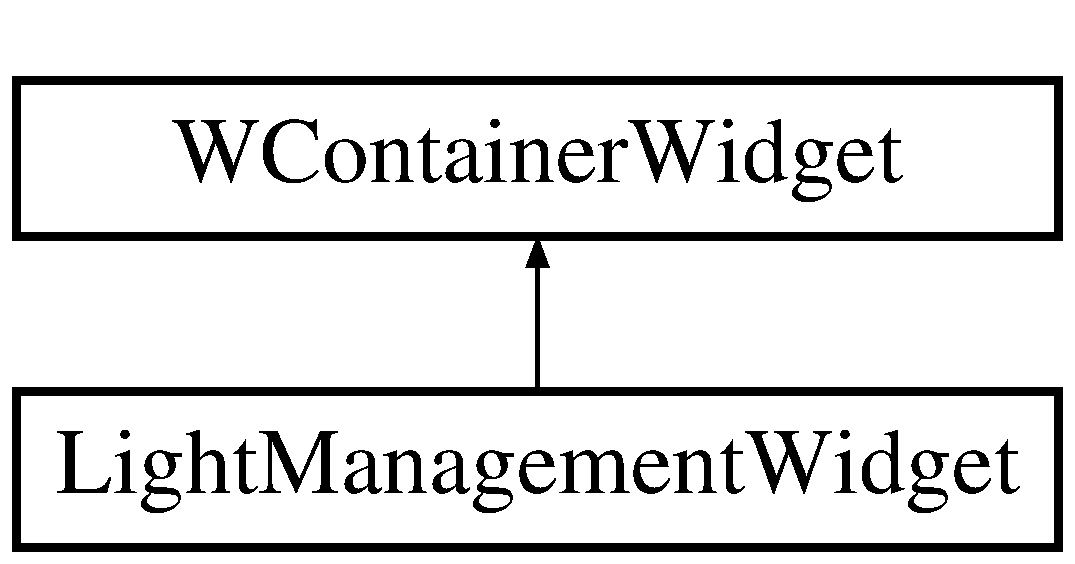
\includegraphics[height=2.000000cm]{classLightManagementWidget}
\end{center}
\end{figure}
\subsection*{Public Member Functions}
\begin{DoxyCompactItemize}
\item 
\hyperlink{classLightManagementWidget_a322acb2556f7ce22b997d32cbc23344b}{Light\+Management\+Widget} (Wt\+::\+W\+Container\+Widget $\ast$parent=0, \hyperlink{classBridge}{Bridge} $\ast$bridge=0, \hyperlink{classWelcomeScreen}{Welcome\+Screen} $\ast$main=0)
\begin{DoxyCompactList}\small\item\em \hyperlink{classLight}{Light} Management Widget constructor. \end{DoxyCompactList}\item 
void \hyperlink{classLightManagementWidget_adc85e9100ac03e670cf0a9dc5d271058}{update} ()
\begin{DoxyCompactList}\small\item\em Update function, clears the widget and re-\/populates with elements of the light management. \end{DoxyCompactList}\end{DoxyCompactItemize}
\subsection*{Private Member Functions}
\begin{DoxyCompactItemize}
\item 
void \hyperlink{classLightManagementWidget_ae2c05678777e26cc117dc9e3b1e6d482}{view\+Overview\+Widget} ()
\begin{DoxyCompactList}\small\item\em View overview function, sets the current widget to the overview widget when clicked on the menu. \end{DoxyCompactList}\item 
void \hyperlink{classLightManagementWidget_acd9a32efacbccb61424056839748c283}{view\+Lights\+Widget} ()
\begin{DoxyCompactList}\small\item\em View lights function, sets the current widget to the light widget when clicked on the menu. \end{DoxyCompactList}\item 
void \hyperlink{classLightManagementWidget_a0ba71461f9463f07373bafff62ce017e}{view\+Groups\+Widget} ()
\begin{DoxyCompactList}\small\item\em View groups function, sets the current widget shown to groups widget when clicked on the menu. \end{DoxyCompactList}\item 
void \hyperlink{classLightManagementWidget_a62809bb5bcf8a5a87ed248d9c5880a6c}{view\+Schedules\+Widget} ()
\begin{DoxyCompactList}\small\item\em View schedule function, sets the current widget shown to schedule widget when clicked on the menu. \end{DoxyCompactList}\item 
void \hyperlink{classLightManagementWidget_a7b49494c162f4e9703469d6519e0dc0a}{edit\+R\+G\+B\+Dialog} (\hyperlink{classLight}{Light} $\ast$light)
\begin{DoxyCompactList}\small\item\em Opens a W\+Dialog box to edit rgb values for the specified light. \end{DoxyCompactList}\item 
void \hyperlink{classLightManagementWidget_a36006718c829f0bbd6c2063dded822bc}{edit\+Hue\+Sat\+Dialog} (\hyperlink{classLight}{Light} $\ast$light)
\begin{DoxyCompactList}\small\item\em Opens a W\+Dialog box to convert hue, saturation, and brightness to rgb color. \end{DoxyCompactList}\item 
void \hyperlink{classLightManagementWidget_a80e917263bea4c99ca9182fb57ce0993}{update\+Lights\+Table} ()
\begin{DoxyCompactList}\small\item\em Update lights table function, clears the current table and re-\/populates it with all the lights that are in the bridge. The user can edit the properties of lights from this table. \end{DoxyCompactList}\item 
void \hyperlink{classLightManagementWidget_ae6de54d491c808a6a85ab9b01be3382b}{edit\+Light\+Dialog} (\hyperlink{classLight}{Light} $\ast$light)
\begin{DoxyCompactList}\small\item\em Edit lights function, when the edit button is clicked, a window where the user can change any property of the selected light appears. \end{DoxyCompactList}\item 
void \hyperlink{classLightManagementWidget_afc4ccdbe0e7fe288e3a76284c304be6f}{remove\+Light} (\hyperlink{classLight}{Light} $\ast$light)
\begin{DoxyCompactList}\small\item\em Remove lights function, removes the selected light from the current bridge. Does not work on Hue Emulator but will work with real bridges. \end{DoxyCompactList}\item 
void \hyperlink{classLightManagementWidget_a9455da3d378d78c2840eafa04ea37294}{update\+Light\+Info} (\hyperlink{classLight}{Light} $\ast$light)
\begin{DoxyCompactList}\small\item\em Update lights function, creates a J\+S\+ON request to change properties of a given light based on user\textquotesingle{}s inputs in the edit light dialog box. \end{DoxyCompactList}\item 
void \hyperlink{classLightManagementWidget_a147fb03b68b3caf8744d10c78b26caff}{update\+Light\+Bri} (W\+Slider $\ast$slider\+\_\+, \hyperlink{classLight}{Light} $\ast$light)
\begin{DoxyCompactList}\small\item\em Update brightness function, creates a J\+S\+ON request to update the selected light\textquotesingle{}s brightness value given the brightness slider\textquotesingle{}s value. \end{DoxyCompactList}\item 
void \hyperlink{classLightManagementWidget_abbb93168a42c74301715f6da39ce0040}{update\+Light\+On} (W\+Push\+Button $\ast$button\+\_\+, \hyperlink{classLight}{Light} $\ast$light)
\begin{DoxyCompactList}\small\item\em Update on/off function, creates a J\+S\+ON request to toggle the selected light\textquotesingle{}s on/off value. \end{DoxyCompactList}\item 
void \hyperlink{classLightManagementWidget_a559f5c7680b14415216e00919c01dd3c}{update\+Light\+XY} (\hyperlink{classLight}{Light} $\ast$light)
\begin{DoxyCompactList}\small\item\em Update light\textquotesingle{}s XY function, creates a J\+S\+ON request to update the selected light\textquotesingle{}s color value given the XY values. \end{DoxyCompactList}\item 
void \hyperlink{classLightManagementWidget_a25f87c6906d4f665f17006189161f8ad}{update\+Light\+HS} (\hyperlink{classLight}{Light} $\ast$light)
\begin{DoxyCompactList}\small\item\em Update HS function, creates a J\+S\+ON request to update the selected light\textquotesingle{}s hue, saturation, brightness, and transition time values. \end{DoxyCompactList}\item 
void \hyperlink{classLightManagementWidget_aaf5913f9aa16aaf3d70c929f606851c1}{update\+Groups\+Table} ()
\begin{DoxyCompactList}\small\item\em Update groups table function, clears the current table and re-\/populates it with all the groups that are in the bridge. \end{DoxyCompactList}\item 
void \hyperlink{classLightManagementWidget_afd405081a296906e278bfbea3f200a97}{create\+Group\+Dialog} ()
\begin{DoxyCompactList}\small\item\em Create groups function, when the create button is clicked, a dialog appears where the user can create a group and select lights to be added to the group. \end{DoxyCompactList}\item 
void \hyperlink{classLightManagementWidget_a76c89408eda6d7a22fff2cd308112912}{group\+Advanced\+Dialog} (\hyperlink{classGroup}{Group} $\ast$group)
\begin{DoxyCompactList}\small\item\em Update groups advanced function, creates a opens a dialog box to change any property of a given group based on user\textquotesingle{}s inputs in the dialog box. \end{DoxyCompactList}\item 
void \hyperlink{classLightManagementWidget_a78e5bc6b0f7f5fbe2fe4bf26f61667a7}{edit\+Group\+Dialog} (\hyperlink{classGroup}{Group} $\ast$group)
\begin{DoxyCompactList}\small\item\em Edit group function, when the edit button is clicked, a window where the user can change lights assigned to the selected group appears. \end{DoxyCompactList}\item 
void \hyperlink{classLightManagementWidget_a0471c906b78aadede7142dc0cfa163aa}{create\+Group} ()
\begin{DoxyCompactList}\small\item\em Create group function, creates a J\+S\+ON request to add a new group to the bridge, using the user defined options selected in create group dialog. \end{DoxyCompactList}\item 
void \hyperlink{classLightManagementWidget_aa05013c523ad75a8e5cf76f1698ce33e}{remove\+Group} (\hyperlink{classGroup}{Group} $\ast$group)
\begin{DoxyCompactList}\small\item\em Remove group function, creates a J\+S\+ON request to remove the selected group from the current bridge. \end{DoxyCompactList}\item 
void \hyperlink{classLightManagementWidget_aa121e339ea3b4b7df1d2c60fffc01cd2}{update\+Group\+Info} (\hyperlink{classGroup}{Group} $\ast$group)
\begin{DoxyCompactList}\small\item\em Update groups function, creates a J\+S\+ON request to change properties of a given group based on user\textquotesingle{}s inputs in the edit group dialog box. \end{DoxyCompactList}\item 
void \hyperlink{classLightManagementWidget_a4515cfa200080a28655aa73f43641cf5}{group\+Update\+Advanced} (\hyperlink{classGroup}{Group} $\ast$group)
\begin{DoxyCompactList}\small\item\em Update groups function, creates a J\+S\+ON request to change properties of a given group based on user\textquotesingle{}s inputs in the advanced group dialog box. \end{DoxyCompactList}\item 
void \hyperlink{classLightManagementWidget_a8269fdb02b41728a474d07830743b61f}{update\+Schedules\+Table} ()
\begin{DoxyCompactList}\small\item\em Update schedules table function, clears the current table and re-\/populates it with all the schedules that are in the bridge. \end{DoxyCompactList}\item 
void \hyperlink{classLightManagementWidget_a387f9ca2f98907351c63ebac6d1e70fe}{create\+Schedule\+Dialog} ()
\begin{DoxyCompactList}\small\item\em Create schedule function, when the create button is clicked, a dialog appears where the user can create a schedule and select their options. \end{DoxyCompactList}\item 
void \hyperlink{classLightManagementWidget_a016342be1f2ecb2f805405d1e68399e7}{create\+Schedule} ()
\begin{DoxyCompactList}\small\item\em Create schedule function, creates a J\+S\+ON request to add a new schedule to the bridge, using the user defined options selected in create schedule dialog. \end{DoxyCompactList}\item 
void \hyperlink{classLightManagementWidget_aaa66e284cf4bbc7c1127ae9d325e41a2}{edit\+Schedule\+Dialog} (\hyperlink{classSchedule}{Schedule} $\ast$schedule)
\begin{DoxyCompactList}\small\item\em Edit schedule function, when the edit button is clicked, a window where the user can change properties for the selected schedule appears. \end{DoxyCompactList}\item 
void \hyperlink{classLightManagementWidget_ac6a0c7163e0e383c55d72490d1ded36b}{update\+Schedule\+Info} (\hyperlink{classSchedule}{Schedule} $\ast$schedule)
\begin{DoxyCompactList}\small\item\em Update schedule function, creates a J\+S\+ON request to change properties of a given schedule based on user\textquotesingle{}s inputs in the edit schedule dialog box. \end{DoxyCompactList}\item 
void \hyperlink{classLightManagementWidget_af654e9b80fa36c3bde02464907d2745e}{remove\+Schedule} (\hyperlink{classSchedule}{Schedule} $\ast$schedule)
\begin{DoxyCompactList}\small\item\em Remove schedule function, creates a J\+S\+ON request to remove the selected schedule from the current bridge. \end{DoxyCompactList}\item 
void \hyperlink{classLightManagementWidget_a0cddaa88f0ec438a61a421d059935048}{delete\+Request} (string url)
\begin{DoxyCompactList}\small\item\em Function that creates a new H\+T\+TP Client and generates a Client D\+E\+L\+E\+TE request to access the Hue A\+PI for the current resource specified in U\+RL. Calls \hyperlink{classLightManagementWidget_a09f20b24e34de1ede968a73e7118913e}{handle\+Put\+Http()} function once client is done the D\+E\+L\+E\+TE call to handle the response. \end{DoxyCompactList}\item 
void \hyperlink{classLightManagementWidget_a13603b45a36df6fc5ffab68bc1791f6f}{put\+Request} (string url, string json)
\begin{DoxyCompactList}\small\item\em Function that creates a new H\+T\+TP Client and generates a Client P\+UT request to access the Hue A\+PI for the current resource specified in U\+RL. Calls \hyperlink{classLightManagementWidget_a09f20b24e34de1ede968a73e7118913e}{handle\+Put\+Http()} function once client is done the P\+UT call to handle the response. \end{DoxyCompactList}\item 
void \hyperlink{classLightManagementWidget_a2d83bd768b2afc25eaade1ca8d64d878}{post\+Request} (string url, string json)
\begin{DoxyCompactList}\small\item\em Function that creates a new H\+T\+TP Client and generates a Client P\+O\+ST request to access the Hue A\+PI for the current resource specified in U\+RL. Calls \hyperlink{classLightManagementWidget_a09f20b24e34de1ede968a73e7118913e}{handle\+Put\+Http()} function once client is done the P\+O\+ST call to handle the response. \end{DoxyCompactList}\item 
void \hyperlink{classLightManagementWidget_a09f20b24e34de1ede968a73e7118913e}{handle\+Put\+Http} (boost\+::system\+::error\+\_\+code err, const Wt\+::\+Http\+::\+Message \&response)
\begin{DoxyCompactList}\small\item\em Function to handle the Http response generated by the Wt Http Client object. This function handles the done() signal sent when doing Client\textquotesingle{}s put, post, and delete\+Request functions even though it is named handle\+Put\+Http. \end{DoxyCompactList}\item 
void \hyperlink{classLightManagementWidget_a6d10a493cf2189f9a949c12828b499c2}{refresh\+Bridge} ()
\begin{DoxyCompactList}\small\item\em Function that creates a new H\+T\+TP Client and generates a Client G\+ET request to access the Hue A\+PI for the current \hyperlink{classBridge}{Bridge}. Calls \hyperlink{classLightManagementWidget_aef0c2a180f37b97769e39a52a9fce257}{refresh\+Bridge\+Http()} function once client is done the G\+ET call to handle the response. \end{DoxyCompactList}\item 
void \hyperlink{classLightManagementWidget_aef0c2a180f37b97769e39a52a9fce257}{refresh\+Bridge\+Http} (boost\+::system\+::error\+\_\+code err, const Wt\+::\+Http\+::\+Message \&response)
\begin{DoxyCompactList}\small\item\em Function to handle the Http response generated by the Wt Http Client object. \end{DoxyCompactList}\end{DoxyCompactItemize}
\subsection*{Private Attributes}
\begin{DoxyCompactItemize}
\item 
\hyperlink{classWelcomeScreen}{Welcome\+Screen} $\ast$ {\bfseries parent\+\_\+}\hypertarget{classLightManagementWidget_a6c29ac9c7547417b442219b962ca2195}{}\label{classLightManagementWidget_a6c29ac9c7547417b442219b962ca2195}

\item 
\hyperlink{classBridge}{Bridge} $\ast$ {\bfseries bridge\+\_\+}\hypertarget{classLightManagementWidget_af55628a2bfe170e6eb56a5630fdd947d}{}\label{classLightManagementWidget_af55628a2bfe170e6eb56a5630fdd947d}

\item 
Wt\+::\+W\+Stacked\+Widget $\ast$ {\bfseries light\+Management\+Stack\+\_\+}\hypertarget{classLightManagementWidget_ae46ca954b273cee2c4ad33bf31137f52}{}\label{classLightManagementWidget_ae46ca954b273cee2c4ad33bf31137f52}

\item 
Wt\+::\+W\+Container\+Widget $\ast$ {\bfseries overview\+Widget\+\_\+}\hypertarget{classLightManagementWidget_a1b1170bf380fc56c67870ecdb0129c27}{}\label{classLightManagementWidget_a1b1170bf380fc56c67870ecdb0129c27}

\item 
Wt\+::\+W\+Container\+Widget $\ast$ {\bfseries lights\+Widget\+\_\+}\hypertarget{classLightManagementWidget_a75b0f44814bba96f4c6c4e2168e2461b}{}\label{classLightManagementWidget_a75b0f44814bba96f4c6c4e2168e2461b}

\item 
Wt\+::\+W\+Container\+Widget $\ast$ {\bfseries groups\+Widget\+\_\+}\hypertarget{classLightManagementWidget_a141e40120063933b98c6dd73a0672d56}{}\label{classLightManagementWidget_a141e40120063933b98c6dd73a0672d56}

\item 
Wt\+::\+W\+Container\+Widget $\ast$ {\bfseries schedules\+Widget\+\_\+}\hypertarget{classLightManagementWidget_abf56d950683122a6f3fda911c4722dfe}{}\label{classLightManagementWidget_abf56d950683122a6f3fda911c4722dfe}

\item 
Wt\+::\+W\+Table $\ast$ {\bfseries lights\+Table\+\_\+}\hypertarget{classLightManagementWidget_a0abd3deb6e9263dc8ed1b3c77c88eb01}{}\label{classLightManagementWidget_a0abd3deb6e9263dc8ed1b3c77c88eb01}

\item 
Wt\+::\+W\+Table $\ast$ {\bfseries groups\+Table\+\_\+}\hypertarget{classLightManagementWidget_aa9b7fa9e000e5593b729bece3a5060d0}{}\label{classLightManagementWidget_aa9b7fa9e000e5593b729bece3a5060d0}

\item 
Wt\+::\+W\+Table $\ast$ {\bfseries schedules\+Table\+\_\+}\hypertarget{classLightManagementWidget_a765cd5781b6e245dbf884ce10b67f188}{}\label{classLightManagementWidget_a765cd5781b6e245dbf884ce10b67f188}

\item 
Wt\+::\+W\+Container\+Widget $\ast$ {\bfseries rgb\+Container\+\_\+}\hypertarget{classLightManagementWidget_a711e78c0659a5a8220605d7352510612}{}\label{classLightManagementWidget_a711e78c0659a5a8220605d7352510612}

\item 
Wt\+::\+W\+Slider $\ast$ {\bfseries brightness\+Slider\+\_\+}\hypertarget{classLightManagementWidget_aa9b9dffea1c57e92e6c76d5504cd258e}{}\label{classLightManagementWidget_aa9b9dffea1c57e92e6c76d5504cd258e}

\item 
Wt\+::\+W\+Dialog $\ast$ {\bfseries edit\+R\+G\+B\+Dialog\+\_\+}\hypertarget{classLightManagementWidget_a4906e9eadc8fa1dc7b9369d36e2a3842}{}\label{classLightManagementWidget_a4906e9eadc8fa1dc7b9369d36e2a3842}

\item 
Wt\+::\+W\+Slider $\ast$ {\bfseries red\+Slider}\hypertarget{classLightManagementWidget_a172179e9792e715c46aee1cef8008712}{}\label{classLightManagementWidget_a172179e9792e715c46aee1cef8008712}

\item 
Wt\+::\+W\+Slider $\ast$ {\bfseries green\+Slider}\hypertarget{classLightManagementWidget_adb06ad0e7fb340d917cc00514932d488}{}\label{classLightManagementWidget_adb06ad0e7fb340d917cc00514932d488}

\item 
Wt\+::\+W\+Slider $\ast$ {\bfseries blue\+Slider}\hypertarget{classLightManagementWidget_a42b38e8361fb5efd81e9186009d401d8}{}\label{classLightManagementWidget_a42b38e8361fb5efd81e9186009d401d8}

\item 
Wt\+::\+W\+Container\+Widget $\ast$ {\bfseries hue\+Sat\+Container\+\_\+}\hypertarget{classLightManagementWidget_a22024c8ee2d5f3124f29f2e15fb3bbc0}{}\label{classLightManagementWidget_a22024c8ee2d5f3124f29f2e15fb3bbc0}

\item 
Wt\+::\+W\+Dialog $\ast$ {\bfseries edit\+Hue\+Sat\+Dialog\+\_\+}\hypertarget{classLightManagementWidget_af901a64435e0440d0f59b824b0b6dacb}{}\label{classLightManagementWidget_af901a64435e0440d0f59b824b0b6dacb}

\item 
Wt\+::\+W\+Slider $\ast$ {\bfseries hue\+Slider}\hypertarget{classLightManagementWidget_a3be0dfb061ca6694babd317a653a834d}{}\label{classLightManagementWidget_a3be0dfb061ca6694babd317a653a834d}

\item 
Wt\+::\+W\+Slider $\ast$ {\bfseries sat\+Slider}\hypertarget{classLightManagementWidget_a5103125086f2e29dc3401f069338fba7}{}\label{classLightManagementWidget_a5103125086f2e29dc3401f069338fba7}

\item 
Wt\+::\+W\+Slider $\ast$ {\bfseries bri\+Slider}\hypertarget{classLightManagementWidget_a6c3438767954e3a44ae771a49c62cf6d}{}\label{classLightManagementWidget_a6c3438767954e3a44ae771a49c62cf6d}

\item 
Wt\+::\+W\+Line\+Edit $\ast$ {\bfseries edit\+Light\+Transition}\hypertarget{classLightManagementWidget_a47d15db8db2b67e467dab491b1d0265f}{}\label{classLightManagementWidget_a47d15db8db2b67e467dab491b1d0265f}

\item 
Wt\+::\+W\+Int\+Validator $\ast$ {\bfseries int\+Validator}\hypertarget{classLightManagementWidget_ac7abebc7258c8c2aa766be0b3204ef65}{}\label{classLightManagementWidget_ac7abebc7258c8c2aa766be0b3204ef65}

\item 
Wt\+::\+W\+Dialog $\ast$ {\bfseries edit\+Light\+Dialog\+\_\+}\hypertarget{classLightManagementWidget_a0563d72b52abb642fab4d986f0e23c10}{}\label{classLightManagementWidget_a0563d72b52abb642fab4d986f0e23c10}

\item 
Wt\+::\+W\+Line\+Edit $\ast$ {\bfseries edit\+Light\+Name}\hypertarget{classLightManagementWidget_a70c73c332969658554a49888b2344935}{}\label{classLightManagementWidget_a70c73c332969658554a49888b2344935}

\item 
Wt\+::\+W\+Dialog $\ast$ {\bfseries create\+Group\+Dialog\+\_\+}\hypertarget{classLightManagementWidget_aba520c3c25b95df6315d48bb5b51453e}{}\label{classLightManagementWidget_aba520c3c25b95df6315d48bb5b51453e}

\item 
Wt\+::\+W\+Line\+Edit $\ast$ {\bfseries group\+Name}\hypertarget{classLightManagementWidget_a9744405ffdd05c9b30d6b83d4f1b244e}{}\label{classLightManagementWidget_a9744405ffdd05c9b30d6b83d4f1b244e}

\item 
vector$<$ W\+Check\+Box $\ast$ $>$ {\bfseries light\+Boxes}\hypertarget{classLightManagementWidget_a6d6106707c59d849fa0611038e0167d7}{}\label{classLightManagementWidget_a6d6106707c59d849fa0611038e0167d7}

\item 
Wt\+::\+W\+Dialog $\ast$ {\bfseries edit\+Group\+Dialog\+\_\+}\hypertarget{classLightManagementWidget_afdd383828277fe7c74fc10ed7e6128b6}{}\label{classLightManagementWidget_afdd383828277fe7c74fc10ed7e6128b6}

\item 
Wt\+::\+W\+Line\+Edit $\ast$ {\bfseries edit\+Group\+Name}\hypertarget{classLightManagementWidget_a79a564dbf36f3c2d30df3278d7d735b8}{}\label{classLightManagementWidget_a79a564dbf36f3c2d30df3278d7d735b8}

\item 
Wt\+::\+W\+Dialog $\ast$ {\bfseries group\+Advanced\+Dialog\+\_\+}\hypertarget{classLightManagementWidget_a81640788de8689669bbe83b4ec071168}{}\label{classLightManagementWidget_a81640788de8689669bbe83b4ec071168}

\item 
Wt\+::\+W\+Slider $\ast$ {\bfseries brightness\+Group}\hypertarget{classLightManagementWidget_a6cb05902dd93f6a3febf3e421ff705fb}{}\label{classLightManagementWidget_a6cb05902dd93f6a3febf3e421ff705fb}

\item 
Wt\+::\+W\+Line\+Edit $\ast$ {\bfseries hue}\hypertarget{classLightManagementWidget_acb714cf811dc41ba76c7bd495b984fc0}{}\label{classLightManagementWidget_acb714cf811dc41ba76c7bd495b984fc0}

\item 
Wt\+::\+W\+Line\+Edit $\ast$ {\bfseries saturation}\hypertarget{classLightManagementWidget_a8d0083dc37a812d1b0eff09be259011b}{}\label{classLightManagementWidget_a8d0083dc37a812d1b0eff09be259011b}

\item 
Wt\+::\+W\+Line\+Edit $\ast$ {\bfseries ct}\hypertarget{classLightManagementWidget_a6a16fc3f7b9329043748049c793415d3}{}\label{classLightManagementWidget_a6a16fc3f7b9329043748049c793415d3}

\item 
Wt\+::\+W\+Combo\+Box $\ast$ {\bfseries alert}\hypertarget{classLightManagementWidget_aef538a35ec1ff1eda77521cfe676993e}{}\label{classLightManagementWidget_aef538a35ec1ff1eda77521cfe676993e}

\item 
Wt\+::\+W\+Combo\+Box $\ast$ {\bfseries effect}\hypertarget{classLightManagementWidget_a56b2612aca4fc546260aa035f1978b04}{}\label{classLightManagementWidget_a56b2612aca4fc546260aa035f1978b04}

\item 
W\+Combo\+Box $\ast$ {\bfseries reachable}\hypertarget{classLightManagementWidget_aeef6a9c220745a7aa9c46788effd386d}{}\label{classLightManagementWidget_aeef6a9c220745a7aa9c46788effd386d}

\item 
Wt\+::\+W\+Dialog $\ast$ {\bfseries create\+Schedule\+Dialog\+\_\+}\hypertarget{classLightManagementWidget_ad1510a03d0e4db44b52826251f0fe986}{}\label{classLightManagementWidget_ad1510a03d0e4db44b52826251f0fe986}

\item 
Wt\+::\+W\+Line\+Edit $\ast$ {\bfseries schedule\+Name}\hypertarget{classLightManagementWidget_aa16ef200e92a2de85f428691b9090ed8}{}\label{classLightManagementWidget_aa16ef200e92a2de85f428691b9090ed8}

\item 
Wt\+::\+W\+Line\+Edit $\ast$ {\bfseries description}\hypertarget{classLightManagementWidget_ad43a0fb4aa96dffe001f3b6f4b43195d}{}\label{classLightManagementWidget_ad43a0fb4aa96dffe001f3b6f4b43195d}

\item 
Wt\+::\+W\+Date\+Edit $\ast$ {\bfseries date\+Edit}\hypertarget{classLightManagementWidget_aecb35c19775f79d3d121cef537939ab0}{}\label{classLightManagementWidget_aecb35c19775f79d3d121cef537939ab0}

\item 
Wt\+::\+W\+Time\+Edit $\ast$ {\bfseries time\+Edit}\hypertarget{classLightManagementWidget_a9c8cbffe6b832365928a20aba96673ff}{}\label{classLightManagementWidget_a9c8cbffe6b832365928a20aba96673ff}

\item 
Wt\+::\+W\+Button\+Group $\ast$ {\bfseries resource\+Button\+Group}\hypertarget{classLightManagementWidget_a220fb38a472e53d77530fc2e3a5be5c4}{}\label{classLightManagementWidget_a220fb38a472e53d77530fc2e3a5be5c4}

\item 
W\+Line\+Edit $\ast$ {\bfseries resource\+Num}\hypertarget{classLightManagementWidget_ad972179df7def919c315d3ef7edf36d0}{}\label{classLightManagementWidget_ad972179df7def919c315d3ef7edf36d0}

\item 
Wt\+::\+W\+Button\+Group $\ast$ {\bfseries action\+Button\+Group}\hypertarget{classLightManagementWidget_ab236b088b3ff8e95e33759fa808b1cbe}{}\label{classLightManagementWidget_ab236b088b3ff8e95e33759fa808b1cbe}

\item 
Wt\+::\+W\+Button\+Group $\ast$ {\bfseries on\+Button\+Group}\hypertarget{classLightManagementWidget_aaee5db1e504e174c479e5cdc0c05f1d8}{}\label{classLightManagementWidget_aaee5db1e504e174c479e5cdc0c05f1d8}

\item 
W\+Slider $\ast$ {\bfseries brightness\+Schedule}\hypertarget{classLightManagementWidget_a43d80104e5a6ebc95306b4f7cc3d0cff}{}\label{classLightManagementWidget_a43d80104e5a6ebc95306b4f7cc3d0cff}

\item 
W\+Line\+Edit $\ast$ {\bfseries transition\+Schedule}\hypertarget{classLightManagementWidget_a866c4bd22470913d82b03a344f9ec85a}{}\label{classLightManagementWidget_a866c4bd22470913d82b03a344f9ec85a}

\item 
Wt\+::\+W\+Dialog $\ast$ {\bfseries edit\+Schedule\+Dialog\+\_\+}\hypertarget{classLightManagementWidget_a7fbc9ed222c8f28e682096bdfa93ceee}{}\label{classLightManagementWidget_a7fbc9ed222c8f28e682096bdfa93ceee}

\item 
Wt\+::\+W\+Line\+Edit $\ast$ {\bfseries edit\+Schedule\+Description}\hypertarget{classLightManagementWidget_a2c5a53051c346b1d611f7ac267789968}{}\label{classLightManagementWidget_a2c5a53051c346b1d611f7ac267789968}

\item 
Wt\+::\+W\+Line\+Edit $\ast$ {\bfseries edit\+Schedule\+Name}\hypertarget{classLightManagementWidget_ab9575daea224ed3c340387d447606360}{}\label{classLightManagementWidget_ab9575daea224ed3c340387d447606360}

\item 
Wt\+::\+W\+Date\+Edit $\ast$ {\bfseries edit\+Date\+Edit}\hypertarget{classLightManagementWidget_a299b7f356c693f7ea7dcbd6f417c0158}{}\label{classLightManagementWidget_a299b7f356c693f7ea7dcbd6f417c0158}

\item 
Wt\+::\+W\+Time\+Edit $\ast$ {\bfseries edit\+Time\+Edit}\hypertarget{classLightManagementWidget_a24a9a2f46f3984db535686c5a5b54035}{}\label{classLightManagementWidget_a24a9a2f46f3984db535686c5a5b54035}

\end{DoxyCompactItemize}


\subsection{Constructor \& Destructor Documentation}
\index{Light\+Management\+Widget@{Light\+Management\+Widget}!Light\+Management\+Widget@{Light\+Management\+Widget}}
\index{Light\+Management\+Widget@{Light\+Management\+Widget}!Light\+Management\+Widget@{Light\+Management\+Widget}}
\subsubsection[{\texorpdfstring{Light\+Management\+Widget(\+Wt\+::\+W\+Container\+Widget $\ast$parent=0, Bridge $\ast$bridge=0, Welcome\+Screen $\ast$main=0)}{LightManagementWidget(Wt::WContainerWidget *parent=0, Bridge *bridge=0, WelcomeScreen *main=0)}}]{\setlength{\rightskip}{0pt plus 5cm}Light\+Management\+Widget\+::\+Light\+Management\+Widget (
\begin{DoxyParamCaption}
\item[{Wt\+::\+W\+Container\+Widget $\ast$}]{parent = {\ttfamily 0}, }
\item[{{\bf Bridge} $\ast$}]{bridge = {\ttfamily 0}, }
\item[{{\bf Welcome\+Screen} $\ast$}]{main = {\ttfamily 0}}
\end{DoxyParamCaption}
)}\hypertarget{classLightManagementWidget_a322acb2556f7ce22b997d32cbc23344b}{}\label{classLightManagementWidget_a322acb2556f7ce22b997d32cbc23344b}


\hyperlink{classLight}{Light} Management Widget constructor. 


\begin{DoxyParams}{Parameters}
{\em $\ast$parent} & is a pointer the the containerwidget that stores this widget \\
\hline
{\em $\ast$bridge} & is a pointer to the \hyperlink{classBridge}{Bridge} object \\
\hline
{\em $\ast$main} & is a pointer to the app\textquotesingle{}s welcome screen \\
\hline
\end{DoxyParams}


\subsection{Member Function Documentation}
\index{Light\+Management\+Widget@{Light\+Management\+Widget}!create\+Group@{create\+Group}}
\index{create\+Group@{create\+Group}!Light\+Management\+Widget@{Light\+Management\+Widget}}
\subsubsection[{\texorpdfstring{create\+Group()}{createGroup()}}]{\setlength{\rightskip}{0pt plus 5cm}void Light\+Management\+Widget\+::create\+Group (
\begin{DoxyParamCaption}
{}
\end{DoxyParamCaption}
)\hspace{0.3cm}{\ttfamily [private]}}\hypertarget{classLightManagementWidget_a0471c906b78aadede7142dc0cfa163aa}{}\label{classLightManagementWidget_a0471c906b78aadede7142dc0cfa163aa}


Create group function, creates a J\+S\+ON request to add a new group to the bridge, using the user defined options selected in create group dialog. 

\begin{DoxyReturn}{Returns}
void 
\end{DoxyReturn}
\index{Light\+Management\+Widget@{Light\+Management\+Widget}!create\+Group\+Dialog@{create\+Group\+Dialog}}
\index{create\+Group\+Dialog@{create\+Group\+Dialog}!Light\+Management\+Widget@{Light\+Management\+Widget}}
\subsubsection[{\texorpdfstring{create\+Group\+Dialog()}{createGroupDialog()}}]{\setlength{\rightskip}{0pt plus 5cm}void Light\+Management\+Widget\+::create\+Group\+Dialog (
\begin{DoxyParamCaption}
{}
\end{DoxyParamCaption}
)\hspace{0.3cm}{\ttfamily [private]}}\hypertarget{classLightManagementWidget_afd405081a296906e278bfbea3f200a97}{}\label{classLightManagementWidget_afd405081a296906e278bfbea3f200a97}


Create groups function, when the create button is clicked, a dialog appears where the user can create a group and select lights to be added to the group. 

\begin{DoxyReturn}{Returns}
void 
\end{DoxyReturn}
\index{Light\+Management\+Widget@{Light\+Management\+Widget}!create\+Schedule@{create\+Schedule}}
\index{create\+Schedule@{create\+Schedule}!Light\+Management\+Widget@{Light\+Management\+Widget}}
\subsubsection[{\texorpdfstring{create\+Schedule()}{createSchedule()}}]{\setlength{\rightskip}{0pt plus 5cm}void Light\+Management\+Widget\+::create\+Schedule (
\begin{DoxyParamCaption}
{}
\end{DoxyParamCaption}
)\hspace{0.3cm}{\ttfamily [private]}}\hypertarget{classLightManagementWidget_a016342be1f2ecb2f805405d1e68399e7}{}\label{classLightManagementWidget_a016342be1f2ecb2f805405d1e68399e7}


Create schedule function, creates a J\+S\+ON request to add a new schedule to the bridge, using the user defined options selected in create schedule dialog. 

\begin{DoxyReturn}{Returns}
void 
\end{DoxyReturn}
\index{Light\+Management\+Widget@{Light\+Management\+Widget}!create\+Schedule\+Dialog@{create\+Schedule\+Dialog}}
\index{create\+Schedule\+Dialog@{create\+Schedule\+Dialog}!Light\+Management\+Widget@{Light\+Management\+Widget}}
\subsubsection[{\texorpdfstring{create\+Schedule\+Dialog()}{createScheduleDialog()}}]{\setlength{\rightskip}{0pt plus 5cm}void Light\+Management\+Widget\+::create\+Schedule\+Dialog (
\begin{DoxyParamCaption}
{}
\end{DoxyParamCaption}
)\hspace{0.3cm}{\ttfamily [private]}}\hypertarget{classLightManagementWidget_a387f9ca2f98907351c63ebac6d1e70fe}{}\label{classLightManagementWidget_a387f9ca2f98907351c63ebac6d1e70fe}


Create schedule function, when the create button is clicked, a dialog appears where the user can create a schedule and select their options. 

\begin{DoxyReturn}{Returns}
void 
\end{DoxyReturn}
\index{Light\+Management\+Widget@{Light\+Management\+Widget}!delete\+Request@{delete\+Request}}
\index{delete\+Request@{delete\+Request}!Light\+Management\+Widget@{Light\+Management\+Widget}}
\subsubsection[{\texorpdfstring{delete\+Request(string url)}{deleteRequest(string url)}}]{\setlength{\rightskip}{0pt plus 5cm}void Light\+Management\+Widget\+::delete\+Request (
\begin{DoxyParamCaption}
\item[{string}]{url}
\end{DoxyParamCaption}
)\hspace{0.3cm}{\ttfamily [private]}}\hypertarget{classLightManagementWidget_a0cddaa88f0ec438a61a421d059935048}{}\label{classLightManagementWidget_a0cddaa88f0ec438a61a421d059935048}


Function that creates a new H\+T\+TP Client and generates a Client D\+E\+L\+E\+TE request to access the Hue A\+PI for the current resource specified in U\+RL. Calls \hyperlink{classLightManagementWidget_a09f20b24e34de1ede968a73e7118913e}{handle\+Put\+Http()} function once client is done the D\+E\+L\+E\+TE call to handle the response. 


\begin{DoxyParams}{Parameters}
{\em url} & the url of the resource to D\+E\+L\+E\+TE\\
\hline
\end{DoxyParams}
\begin{DoxyReturn}{Returns}
void 
\end{DoxyReturn}
\index{Light\+Management\+Widget@{Light\+Management\+Widget}!edit\+Group\+Dialog@{edit\+Group\+Dialog}}
\index{edit\+Group\+Dialog@{edit\+Group\+Dialog}!Light\+Management\+Widget@{Light\+Management\+Widget}}
\subsubsection[{\texorpdfstring{edit\+Group\+Dialog(\+Group $\ast$group)}{editGroupDialog(Group *group)}}]{\setlength{\rightskip}{0pt plus 5cm}void Light\+Management\+Widget\+::edit\+Group\+Dialog (
\begin{DoxyParamCaption}
\item[{{\bf Group} $\ast$}]{group}
\end{DoxyParamCaption}
)\hspace{0.3cm}{\ttfamily [private]}}\hypertarget{classLightManagementWidget_a78e5bc6b0f7f5fbe2fe4bf26f61667a7}{}\label{classLightManagementWidget_a78e5bc6b0f7f5fbe2fe4bf26f61667a7}


Edit group function, when the edit button is clicked, a window where the user can change lights assigned to the selected group appears. 


\begin{DoxyParams}{Parameters}
{\em group} & is the group object that was selected to edit from the table.\\
\hline
\end{DoxyParams}
\begin{DoxyReturn}{Returns}
void 
\end{DoxyReturn}
\index{Light\+Management\+Widget@{Light\+Management\+Widget}!edit\+Hue\+Sat\+Dialog@{edit\+Hue\+Sat\+Dialog}}
\index{edit\+Hue\+Sat\+Dialog@{edit\+Hue\+Sat\+Dialog}!Light\+Management\+Widget@{Light\+Management\+Widget}}
\subsubsection[{\texorpdfstring{edit\+Hue\+Sat\+Dialog(\+Light $\ast$light)}{editHueSatDialog(Light *light)}}]{\setlength{\rightskip}{0pt plus 5cm}void Light\+Management\+Widget\+::edit\+Hue\+Sat\+Dialog (
\begin{DoxyParamCaption}
\item[{{\bf Light} $\ast$}]{light}
\end{DoxyParamCaption}
)\hspace{0.3cm}{\ttfamily [private]}}\hypertarget{classLightManagementWidget_a36006718c829f0bbd6c2063dded822bc}{}\label{classLightManagementWidget_a36006718c829f0bbd6c2063dded822bc}


Opens a W\+Dialog box to convert hue, saturation, and brightness to rgb color. 


\begin{DoxyParams}{Parameters}
{\em light} & is the current light object to edit\\
\hline
\end{DoxyParams}
\begin{DoxyReturn}{Returns}
void 
\end{DoxyReturn}
\index{Light\+Management\+Widget@{Light\+Management\+Widget}!edit\+Light\+Dialog@{edit\+Light\+Dialog}}
\index{edit\+Light\+Dialog@{edit\+Light\+Dialog}!Light\+Management\+Widget@{Light\+Management\+Widget}}
\subsubsection[{\texorpdfstring{edit\+Light\+Dialog(\+Light $\ast$light)}{editLightDialog(Light *light)}}]{\setlength{\rightskip}{0pt plus 5cm}void Light\+Management\+Widget\+::edit\+Light\+Dialog (
\begin{DoxyParamCaption}
\item[{{\bf Light} $\ast$}]{light}
\end{DoxyParamCaption}
)\hspace{0.3cm}{\ttfamily [private]}}\hypertarget{classLightManagementWidget_ae6de54d491c808a6a85ab9b01be3382b}{}\label{classLightManagementWidget_ae6de54d491c808a6a85ab9b01be3382b}


Edit lights function, when the edit button is clicked, a window where the user can change any property of the selected light appears. 


\begin{DoxyParams}{Parameters}
{\em light} & is the light object that was selected to edit from the table.\\
\hline
\end{DoxyParams}
\begin{DoxyReturn}{Returns}
void 
\end{DoxyReturn}
\index{Light\+Management\+Widget@{Light\+Management\+Widget}!edit\+R\+G\+B\+Dialog@{edit\+R\+G\+B\+Dialog}}
\index{edit\+R\+G\+B\+Dialog@{edit\+R\+G\+B\+Dialog}!Light\+Management\+Widget@{Light\+Management\+Widget}}
\subsubsection[{\texorpdfstring{edit\+R\+G\+B\+Dialog(\+Light $\ast$light)}{editRGBDialog(Light *light)}}]{\setlength{\rightskip}{0pt plus 5cm}void Light\+Management\+Widget\+::edit\+R\+G\+B\+Dialog (
\begin{DoxyParamCaption}
\item[{{\bf Light} $\ast$}]{light}
\end{DoxyParamCaption}
)\hspace{0.3cm}{\ttfamily [private]}}\hypertarget{classLightManagementWidget_a7b49494c162f4e9703469d6519e0dc0a}{}\label{classLightManagementWidget_a7b49494c162f4e9703469d6519e0dc0a}


Opens a W\+Dialog box to edit rgb values for the specified light. 


\begin{DoxyParams}{Parameters}
{\em light} & is the current light object to edit\\
\hline
\end{DoxyParams}
\begin{DoxyReturn}{Returns}
void 
\end{DoxyReturn}
\index{Light\+Management\+Widget@{Light\+Management\+Widget}!edit\+Schedule\+Dialog@{edit\+Schedule\+Dialog}}
\index{edit\+Schedule\+Dialog@{edit\+Schedule\+Dialog}!Light\+Management\+Widget@{Light\+Management\+Widget}}
\subsubsection[{\texorpdfstring{edit\+Schedule\+Dialog(\+Schedule $\ast$schedule)}{editScheduleDialog(Schedule *schedule)}}]{\setlength{\rightskip}{0pt plus 5cm}void Light\+Management\+Widget\+::edit\+Schedule\+Dialog (
\begin{DoxyParamCaption}
\item[{{\bf Schedule} $\ast$}]{schedule}
\end{DoxyParamCaption}
)\hspace{0.3cm}{\ttfamily [private]}}\hypertarget{classLightManagementWidget_aaa66e284cf4bbc7c1127ae9d325e41a2}{}\label{classLightManagementWidget_aaa66e284cf4bbc7c1127ae9d325e41a2}


Edit schedule function, when the edit button is clicked, a window where the user can change properties for the selected schedule appears. 


\begin{DoxyParams}{Parameters}
{\em schedule} & is the schedule object that was selected to edit from the table.\\
\hline
\end{DoxyParams}
\begin{DoxyReturn}{Returns}
void 
\end{DoxyReturn}
\index{Light\+Management\+Widget@{Light\+Management\+Widget}!group\+Advanced\+Dialog@{group\+Advanced\+Dialog}}
\index{group\+Advanced\+Dialog@{group\+Advanced\+Dialog}!Light\+Management\+Widget@{Light\+Management\+Widget}}
\subsubsection[{\texorpdfstring{group\+Advanced\+Dialog(\+Group $\ast$group)}{groupAdvancedDialog(Group *group)}}]{\setlength{\rightskip}{0pt plus 5cm}void Light\+Management\+Widget\+::group\+Advanced\+Dialog (
\begin{DoxyParamCaption}
\item[{{\bf Group} $\ast$}]{group}
\end{DoxyParamCaption}
)\hspace{0.3cm}{\ttfamily [private]}}\hypertarget{classLightManagementWidget_a76c89408eda6d7a22fff2cd308112912}{}\label{classLightManagementWidget_a76c89408eda6d7a22fff2cd308112912}


Update groups advanced function, creates a opens a dialog box to change any property of a given group based on user\textquotesingle{}s inputs in the dialog box. 


\begin{DoxyParams}{Parameters}
{\em group} & is the group object to update from the bridge.\\
\hline
\end{DoxyParams}
\begin{DoxyReturn}{Returns}
void 
\end{DoxyReturn}
\index{Light\+Management\+Widget@{Light\+Management\+Widget}!group\+Update\+Advanced@{group\+Update\+Advanced}}
\index{group\+Update\+Advanced@{group\+Update\+Advanced}!Light\+Management\+Widget@{Light\+Management\+Widget}}
\subsubsection[{\texorpdfstring{group\+Update\+Advanced(\+Group $\ast$group)}{groupUpdateAdvanced(Group *group)}}]{\setlength{\rightskip}{0pt plus 5cm}void Light\+Management\+Widget\+::group\+Update\+Advanced (
\begin{DoxyParamCaption}
\item[{{\bf Group} $\ast$}]{group}
\end{DoxyParamCaption}
)\hspace{0.3cm}{\ttfamily [private]}}\hypertarget{classLightManagementWidget_a4515cfa200080a28655aa73f43641cf5}{}\label{classLightManagementWidget_a4515cfa200080a28655aa73f43641cf5}


Update groups function, creates a J\+S\+ON request to change properties of a given group based on user\textquotesingle{}s inputs in the advanced group dialog box. 


\begin{DoxyParams}{Parameters}
{\em light} & is the light object to update from the bridge.\\
\hline
\end{DoxyParams}
\begin{DoxyReturn}{Returns}
void 
\end{DoxyReturn}
\index{Light\+Management\+Widget@{Light\+Management\+Widget}!handle\+Put\+Http@{handle\+Put\+Http}}
\index{handle\+Put\+Http@{handle\+Put\+Http}!Light\+Management\+Widget@{Light\+Management\+Widget}}
\subsubsection[{\texorpdfstring{handle\+Put\+Http(boost\+::system\+::error\+\_\+code err, const Wt\+::\+Http\+::\+Message \&response)}{handlePutHttp(boost::system::error_code err, const Wt::Http::Message &response)}}]{\setlength{\rightskip}{0pt plus 5cm}void Light\+Management\+Widget\+::handle\+Put\+Http (
\begin{DoxyParamCaption}
\item[{boost\+::system\+::error\+\_\+code}]{err, }
\item[{const Wt\+::\+Http\+::\+Message \&}]{response}
\end{DoxyParamCaption}
)\hspace{0.3cm}{\ttfamily [private]}}\hypertarget{classLightManagementWidget_a09f20b24e34de1ede968a73e7118913e}{}\label{classLightManagementWidget_a09f20b24e34de1ede968a73e7118913e}


Function to handle the Http response generated by the Wt Http Client object. This function handles the done() signal sent when doing Client\textquotesingle{}s put, post, and delete\+Request functions even though it is named handle\+Put\+Http. 


\begin{DoxyParams}{Parameters}
{\em $\ast$err} & stores the error code generated by an Http request, null if request was successful \\
\hline
{\em \&response} & stores the response message generated by the Http request\\
\hline
\end{DoxyParams}
\begin{DoxyReturn}{Returns}
void 
\end{DoxyReturn}
\index{Light\+Management\+Widget@{Light\+Management\+Widget}!post\+Request@{post\+Request}}
\index{post\+Request@{post\+Request}!Light\+Management\+Widget@{Light\+Management\+Widget}}
\subsubsection[{\texorpdfstring{post\+Request(string url, string json)}{postRequest(string url, string json)}}]{\setlength{\rightskip}{0pt plus 5cm}void Light\+Management\+Widget\+::post\+Request (
\begin{DoxyParamCaption}
\item[{string}]{url, }
\item[{string}]{json}
\end{DoxyParamCaption}
)\hspace{0.3cm}{\ttfamily [private]}}\hypertarget{classLightManagementWidget_a2d83bd768b2afc25eaade1ca8d64d878}{}\label{classLightManagementWidget_a2d83bd768b2afc25eaade1ca8d64d878}


Function that creates a new H\+T\+TP Client and generates a Client P\+O\+ST request to access the Hue A\+PI for the current resource specified in U\+RL. Calls \hyperlink{classLightManagementWidget_a09f20b24e34de1ede968a73e7118913e}{handle\+Put\+Http()} function once client is done the P\+O\+ST call to handle the response. 


\begin{DoxyParams}{Parameters}
{\em url} & the url of the resource to P\+O\+ST the json data to \\
\hline
{\em json} & the body json data to P\+O\+ST to the Hue A\+PI\\
\hline
\end{DoxyParams}
\begin{DoxyReturn}{Returns}
void 
\end{DoxyReturn}
\index{Light\+Management\+Widget@{Light\+Management\+Widget}!put\+Request@{put\+Request}}
\index{put\+Request@{put\+Request}!Light\+Management\+Widget@{Light\+Management\+Widget}}
\subsubsection[{\texorpdfstring{put\+Request(string url, string json)}{putRequest(string url, string json)}}]{\setlength{\rightskip}{0pt plus 5cm}void Light\+Management\+Widget\+::put\+Request (
\begin{DoxyParamCaption}
\item[{string}]{url, }
\item[{string}]{json}
\end{DoxyParamCaption}
)\hspace{0.3cm}{\ttfamily [private]}}\hypertarget{classLightManagementWidget_a13603b45a36df6fc5ffab68bc1791f6f}{}\label{classLightManagementWidget_a13603b45a36df6fc5ffab68bc1791f6f}


Function that creates a new H\+T\+TP Client and generates a Client P\+UT request to access the Hue A\+PI for the current resource specified in U\+RL. Calls \hyperlink{classLightManagementWidget_a09f20b24e34de1ede968a73e7118913e}{handle\+Put\+Http()} function once client is done the P\+UT call to handle the response. 


\begin{DoxyParams}{Parameters}
{\em url} & the url of the resource to P\+UT the json data to \\
\hline
{\em json} & the body json data to P\+UT to the Hue A\+PI\\
\hline
\end{DoxyParams}
\begin{DoxyReturn}{Returns}
void 
\end{DoxyReturn}
\index{Light\+Management\+Widget@{Light\+Management\+Widget}!refresh\+Bridge@{refresh\+Bridge}}
\index{refresh\+Bridge@{refresh\+Bridge}!Light\+Management\+Widget@{Light\+Management\+Widget}}
\subsubsection[{\texorpdfstring{refresh\+Bridge()}{refreshBridge()}}]{\setlength{\rightskip}{0pt plus 5cm}void Light\+Management\+Widget\+::refresh\+Bridge (
\begin{DoxyParamCaption}
{}
\end{DoxyParamCaption}
)\hspace{0.3cm}{\ttfamily [private]}}\hypertarget{classLightManagementWidget_a6d10a493cf2189f9a949c12828b499c2}{}\label{classLightManagementWidget_a6d10a493cf2189f9a949c12828b499c2}


Function that creates a new H\+T\+TP Client and generates a Client G\+ET request to access the Hue A\+PI for the current \hyperlink{classBridge}{Bridge}. Calls \hyperlink{classLightManagementWidget_aef0c2a180f37b97769e39a52a9fce257}{refresh\+Bridge\+Http()} function once client is done the G\+ET call to handle the response. 

\begin{DoxyReturn}{Returns}
void 
\end{DoxyReturn}
\index{Light\+Management\+Widget@{Light\+Management\+Widget}!refresh\+Bridge\+Http@{refresh\+Bridge\+Http}}
\index{refresh\+Bridge\+Http@{refresh\+Bridge\+Http}!Light\+Management\+Widget@{Light\+Management\+Widget}}
\subsubsection[{\texorpdfstring{refresh\+Bridge\+Http(boost\+::system\+::error\+\_\+code err, const Wt\+::\+Http\+::\+Message \&response)}{refreshBridgeHttp(boost::system::error_code err, const Wt::Http::Message &response)}}]{\setlength{\rightskip}{0pt plus 5cm}void Light\+Management\+Widget\+::refresh\+Bridge\+Http (
\begin{DoxyParamCaption}
\item[{boost\+::system\+::error\+\_\+code}]{err, }
\item[{const Wt\+::\+Http\+::\+Message \&}]{response}
\end{DoxyParamCaption}
)\hspace{0.3cm}{\ttfamily [private]}}\hypertarget{classLightManagementWidget_aef0c2a180f37b97769e39a52a9fce257}{}\label{classLightManagementWidget_aef0c2a180f37b97769e39a52a9fce257}


Function to handle the Http response generated by the Wt Http Client object. 


\begin{DoxyParams}{Parameters}
{\em $\ast$err} & stores the error code generated by an Http request, null if request was successful \\
\hline
{\em \&response} & stores the response message generated by the Http request\\
\hline
\end{DoxyParams}
\begin{DoxyReturn}{Returns}
void 
\end{DoxyReturn}
\index{Light\+Management\+Widget@{Light\+Management\+Widget}!remove\+Group@{remove\+Group}}
\index{remove\+Group@{remove\+Group}!Light\+Management\+Widget@{Light\+Management\+Widget}}
\subsubsection[{\texorpdfstring{remove\+Group(\+Group $\ast$group)}{removeGroup(Group *group)}}]{\setlength{\rightskip}{0pt plus 5cm}void Light\+Management\+Widget\+::remove\+Group (
\begin{DoxyParamCaption}
\item[{{\bf Group} $\ast$}]{group}
\end{DoxyParamCaption}
)\hspace{0.3cm}{\ttfamily [private]}}\hypertarget{classLightManagementWidget_aa05013c523ad75a8e5cf76f1698ce33e}{}\label{classLightManagementWidget_aa05013c523ad75a8e5cf76f1698ce33e}


Remove group function, creates a J\+S\+ON request to remove the selected group from the current bridge. 


\begin{DoxyParams}{Parameters}
{\em group} & is the group object to remove from the bridge.\\
\hline
\end{DoxyParams}
\begin{DoxyReturn}{Returns}
void 
\end{DoxyReturn}
\index{Light\+Management\+Widget@{Light\+Management\+Widget}!remove\+Light@{remove\+Light}}
\index{remove\+Light@{remove\+Light}!Light\+Management\+Widget@{Light\+Management\+Widget}}
\subsubsection[{\texorpdfstring{remove\+Light(\+Light $\ast$light)}{removeLight(Light *light)}}]{\setlength{\rightskip}{0pt plus 5cm}void Light\+Management\+Widget\+::remove\+Light (
\begin{DoxyParamCaption}
\item[{{\bf Light} $\ast$}]{light}
\end{DoxyParamCaption}
)\hspace{0.3cm}{\ttfamily [private]}}\hypertarget{classLightManagementWidget_afc4ccdbe0e7fe288e3a76284c304be6f}{}\label{classLightManagementWidget_afc4ccdbe0e7fe288e3a76284c304be6f}


Remove lights function, removes the selected light from the current bridge. Does not work on Hue Emulator but will work with real bridges. 


\begin{DoxyParams}{Parameters}
{\em light} & is the light object to remove from the bridge.\\
\hline
\end{DoxyParams}
\begin{DoxyReturn}{Returns}
void 
\end{DoxyReturn}
\index{Light\+Management\+Widget@{Light\+Management\+Widget}!remove\+Schedule@{remove\+Schedule}}
\index{remove\+Schedule@{remove\+Schedule}!Light\+Management\+Widget@{Light\+Management\+Widget}}
\subsubsection[{\texorpdfstring{remove\+Schedule(\+Schedule $\ast$schedule)}{removeSchedule(Schedule *schedule)}}]{\setlength{\rightskip}{0pt plus 5cm}void Light\+Management\+Widget\+::remove\+Schedule (
\begin{DoxyParamCaption}
\item[{{\bf Schedule} $\ast$}]{schedule}
\end{DoxyParamCaption}
)\hspace{0.3cm}{\ttfamily [private]}}\hypertarget{classLightManagementWidget_af654e9b80fa36c3bde02464907d2745e}{}\label{classLightManagementWidget_af654e9b80fa36c3bde02464907d2745e}


Remove schedule function, creates a J\+S\+ON request to remove the selected schedule from the current bridge. 


\begin{DoxyParams}{Parameters}
{\em schedule} & is the schedule object to remove from the bridge.\\
\hline
\end{DoxyParams}
\begin{DoxyReturn}{Returns}
void 
\end{DoxyReturn}
\index{Light\+Management\+Widget@{Light\+Management\+Widget}!update@{update}}
\index{update@{update}!Light\+Management\+Widget@{Light\+Management\+Widget}}
\subsubsection[{\texorpdfstring{update()}{update()}}]{\setlength{\rightskip}{0pt plus 5cm}void Light\+Management\+Widget\+::update (
\begin{DoxyParamCaption}
{}
\end{DoxyParamCaption}
)}\hypertarget{classLightManagementWidget_adc85e9100ac03e670cf0a9dc5d271058}{}\label{classLightManagementWidget_adc85e9100ac03e670cf0a9dc5d271058}


Update function, clears the widget and re-\/populates with elements of the light management. 

\begin{DoxyReturn}{Returns}
void 
\end{DoxyReturn}
\index{Light\+Management\+Widget@{Light\+Management\+Widget}!update\+Group\+Info@{update\+Group\+Info}}
\index{update\+Group\+Info@{update\+Group\+Info}!Light\+Management\+Widget@{Light\+Management\+Widget}}
\subsubsection[{\texorpdfstring{update\+Group\+Info(\+Group $\ast$group)}{updateGroupInfo(Group *group)}}]{\setlength{\rightskip}{0pt plus 5cm}void Light\+Management\+Widget\+::update\+Group\+Info (
\begin{DoxyParamCaption}
\item[{{\bf Group} $\ast$}]{group}
\end{DoxyParamCaption}
)\hspace{0.3cm}{\ttfamily [private]}}\hypertarget{classLightManagementWidget_aa121e339ea3b4b7df1d2c60fffc01cd2}{}\label{classLightManagementWidget_aa121e339ea3b4b7df1d2c60fffc01cd2}


Update groups function, creates a J\+S\+ON request to change properties of a given group based on user\textquotesingle{}s inputs in the edit group dialog box. 


\begin{DoxyParams}{Parameters}
{\em group} & is the group object to update from the bridge.\\
\hline
\end{DoxyParams}
\begin{DoxyReturn}{Returns}
void 
\end{DoxyReturn}
\index{Light\+Management\+Widget@{Light\+Management\+Widget}!update\+Groups\+Table@{update\+Groups\+Table}}
\index{update\+Groups\+Table@{update\+Groups\+Table}!Light\+Management\+Widget@{Light\+Management\+Widget}}
\subsubsection[{\texorpdfstring{update\+Groups\+Table()}{updateGroupsTable()}}]{\setlength{\rightskip}{0pt plus 5cm}void Light\+Management\+Widget\+::update\+Groups\+Table (
\begin{DoxyParamCaption}
{}
\end{DoxyParamCaption}
)\hspace{0.3cm}{\ttfamily [private]}}\hypertarget{classLightManagementWidget_aaf5913f9aa16aaf3d70c929f606851c1}{}\label{classLightManagementWidget_aaf5913f9aa16aaf3d70c929f606851c1}


Update groups table function, clears the current table and re-\/populates it with all the groups that are in the bridge. 

\begin{DoxyReturn}{Returns}
void 
\end{DoxyReturn}
\index{Light\+Management\+Widget@{Light\+Management\+Widget}!update\+Light\+Bri@{update\+Light\+Bri}}
\index{update\+Light\+Bri@{update\+Light\+Bri}!Light\+Management\+Widget@{Light\+Management\+Widget}}
\subsubsection[{\texorpdfstring{update\+Light\+Bri(\+W\+Slider $\ast$slider\+\_\+, Light $\ast$light)}{updateLightBri(WSlider *slider_, Light *light)}}]{\setlength{\rightskip}{0pt plus 5cm}void Light\+Management\+Widget\+::update\+Light\+Bri (
\begin{DoxyParamCaption}
\item[{W\+Slider $\ast$}]{slider\+\_\+, }
\item[{{\bf Light} $\ast$}]{light}
\end{DoxyParamCaption}
)\hspace{0.3cm}{\ttfamily [private]}}\hypertarget{classLightManagementWidget_a147fb03b68b3caf8744d10c78b26caff}{}\label{classLightManagementWidget_a147fb03b68b3caf8744d10c78b26caff}


Update brightness function, creates a J\+S\+ON request to update the selected light\textquotesingle{}s brightness value given the brightness slider\textquotesingle{}s value. 


\begin{DoxyParams}{Parameters}
{\em slider\+\_\+} & is the brightness slider that contains a value between 0-\/254. \\
\hline
{\em light} & is the light object to update the brightness value.\\
\hline
\end{DoxyParams}
\begin{DoxyReturn}{Returns}
void 
\end{DoxyReturn}
\index{Light\+Management\+Widget@{Light\+Management\+Widget}!update\+Light\+HS@{update\+Light\+HS}}
\index{update\+Light\+HS@{update\+Light\+HS}!Light\+Management\+Widget@{Light\+Management\+Widget}}
\subsubsection[{\texorpdfstring{update\+Light\+H\+S(\+Light $\ast$light)}{updateLightHS(Light *light)}}]{\setlength{\rightskip}{0pt plus 5cm}void Light\+Management\+Widget\+::update\+Light\+HS (
\begin{DoxyParamCaption}
\item[{{\bf Light} $\ast$}]{light}
\end{DoxyParamCaption}
)\hspace{0.3cm}{\ttfamily [private]}}\hypertarget{classLightManagementWidget_a25f87c6906d4f665f17006189161f8ad}{}\label{classLightManagementWidget_a25f87c6906d4f665f17006189161f8ad}


Update HS function, creates a J\+S\+ON request to update the selected light\textquotesingle{}s hue, saturation, brightness, and transition time values. 


\begin{DoxyParams}{Parameters}
{\em light} & is the light object to update.\\
\hline
\end{DoxyParams}
\begin{DoxyReturn}{Returns}
void 
\end{DoxyReturn}
\index{Light\+Management\+Widget@{Light\+Management\+Widget}!update\+Light\+Info@{update\+Light\+Info}}
\index{update\+Light\+Info@{update\+Light\+Info}!Light\+Management\+Widget@{Light\+Management\+Widget}}
\subsubsection[{\texorpdfstring{update\+Light\+Info(\+Light $\ast$light)}{updateLightInfo(Light *light)}}]{\setlength{\rightskip}{0pt plus 5cm}void Light\+Management\+Widget\+::update\+Light\+Info (
\begin{DoxyParamCaption}
\item[{{\bf Light} $\ast$}]{light}
\end{DoxyParamCaption}
)\hspace{0.3cm}{\ttfamily [private]}}\hypertarget{classLightManagementWidget_a9455da3d378d78c2840eafa04ea37294}{}\label{classLightManagementWidget_a9455da3d378d78c2840eafa04ea37294}


Update lights function, creates a J\+S\+ON request to change properties of a given light based on user\textquotesingle{}s inputs in the edit light dialog box. 


\begin{DoxyParams}{Parameters}
{\em light} & is the light object to update from the bridge.\\
\hline
\end{DoxyParams}
\begin{DoxyReturn}{Returns}
void 
\end{DoxyReturn}
\index{Light\+Management\+Widget@{Light\+Management\+Widget}!update\+Light\+On@{update\+Light\+On}}
\index{update\+Light\+On@{update\+Light\+On}!Light\+Management\+Widget@{Light\+Management\+Widget}}
\subsubsection[{\texorpdfstring{update\+Light\+On(\+W\+Push\+Button $\ast$button\+\_\+, Light $\ast$light)}{updateLightOn(WPushButton *button_, Light *light)}}]{\setlength{\rightskip}{0pt plus 5cm}void Light\+Management\+Widget\+::update\+Light\+On (
\begin{DoxyParamCaption}
\item[{W\+Push\+Button $\ast$}]{button\+\_\+, }
\item[{{\bf Light} $\ast$}]{light}
\end{DoxyParamCaption}
)\hspace{0.3cm}{\ttfamily [private]}}\hypertarget{classLightManagementWidget_abbb93168a42c74301715f6da39ce0040}{}\label{classLightManagementWidget_abbb93168a42c74301715f6da39ce0040}


Update on/off function, creates a J\+S\+ON request to toggle the selected light\textquotesingle{}s on/off value. 


\begin{DoxyParams}{Parameters}
{\em button\+\_\+} & is the clickable button that contains on/off value. \\
\hline
{\em light} & is the light object to update the on/off value.\\
\hline
\end{DoxyParams}
\begin{DoxyReturn}{Returns}
void 
\end{DoxyReturn}
\index{Light\+Management\+Widget@{Light\+Management\+Widget}!update\+Lights\+Table@{update\+Lights\+Table}}
\index{update\+Lights\+Table@{update\+Lights\+Table}!Light\+Management\+Widget@{Light\+Management\+Widget}}
\subsubsection[{\texorpdfstring{update\+Lights\+Table()}{updateLightsTable()}}]{\setlength{\rightskip}{0pt plus 5cm}void Light\+Management\+Widget\+::update\+Lights\+Table (
\begin{DoxyParamCaption}
{}
\end{DoxyParamCaption}
)\hspace{0.3cm}{\ttfamily [private]}}\hypertarget{classLightManagementWidget_a80e917263bea4c99ca9182fb57ce0993}{}\label{classLightManagementWidget_a80e917263bea4c99ca9182fb57ce0993}


Update lights table function, clears the current table and re-\/populates it with all the lights that are in the bridge. The user can edit the properties of lights from this table. 

\begin{DoxyReturn}{Returns}
void 
\end{DoxyReturn}
\index{Light\+Management\+Widget@{Light\+Management\+Widget}!update\+Light\+XY@{update\+Light\+XY}}
\index{update\+Light\+XY@{update\+Light\+XY}!Light\+Management\+Widget@{Light\+Management\+Widget}}
\subsubsection[{\texorpdfstring{update\+Light\+X\+Y(\+Light $\ast$light)}{updateLightXY(Light *light)}}]{\setlength{\rightskip}{0pt plus 5cm}void Light\+Management\+Widget\+::update\+Light\+XY (
\begin{DoxyParamCaption}
\item[{{\bf Light} $\ast$}]{light}
\end{DoxyParamCaption}
)\hspace{0.3cm}{\ttfamily [private]}}\hypertarget{classLightManagementWidget_a559f5c7680b14415216e00919c01dd3c}{}\label{classLightManagementWidget_a559f5c7680b14415216e00919c01dd3c}


Update light\textquotesingle{}s XY function, creates a J\+S\+ON request to update the selected light\textquotesingle{}s color value given the XY values. 


\begin{DoxyParams}{Parameters}
{\em light} & is the light object to update the XY value.\\
\hline
\end{DoxyParams}
\begin{DoxyReturn}{Returns}
void 
\end{DoxyReturn}
\index{Light\+Management\+Widget@{Light\+Management\+Widget}!update\+Schedule\+Info@{update\+Schedule\+Info}}
\index{update\+Schedule\+Info@{update\+Schedule\+Info}!Light\+Management\+Widget@{Light\+Management\+Widget}}
\subsubsection[{\texorpdfstring{update\+Schedule\+Info(\+Schedule $\ast$schedule)}{updateScheduleInfo(Schedule *schedule)}}]{\setlength{\rightskip}{0pt plus 5cm}void Light\+Management\+Widget\+::update\+Schedule\+Info (
\begin{DoxyParamCaption}
\item[{{\bf Schedule} $\ast$}]{schedule}
\end{DoxyParamCaption}
)\hspace{0.3cm}{\ttfamily [private]}}\hypertarget{classLightManagementWidget_ac6a0c7163e0e383c55d72490d1ded36b}{}\label{classLightManagementWidget_ac6a0c7163e0e383c55d72490d1ded36b}


Update schedule function, creates a J\+S\+ON request to change properties of a given schedule based on user\textquotesingle{}s inputs in the edit schedule dialog box. 


\begin{DoxyParams}{Parameters}
{\em schedule} & is the schedule object to update from the bridge.\\
\hline
\end{DoxyParams}
\begin{DoxyReturn}{Returns}
void 
\end{DoxyReturn}
\index{Light\+Management\+Widget@{Light\+Management\+Widget}!update\+Schedules\+Table@{update\+Schedules\+Table}}
\index{update\+Schedules\+Table@{update\+Schedules\+Table}!Light\+Management\+Widget@{Light\+Management\+Widget}}
\subsubsection[{\texorpdfstring{update\+Schedules\+Table()}{updateSchedulesTable()}}]{\setlength{\rightskip}{0pt plus 5cm}void Light\+Management\+Widget\+::update\+Schedules\+Table (
\begin{DoxyParamCaption}
{}
\end{DoxyParamCaption}
)\hspace{0.3cm}{\ttfamily [private]}}\hypertarget{classLightManagementWidget_a8269fdb02b41728a474d07830743b61f}{}\label{classLightManagementWidget_a8269fdb02b41728a474d07830743b61f}


Update schedules table function, clears the current table and re-\/populates it with all the schedules that are in the bridge. 

\begin{DoxyReturn}{Returns}
void 
\end{DoxyReturn}
\index{Light\+Management\+Widget@{Light\+Management\+Widget}!view\+Groups\+Widget@{view\+Groups\+Widget}}
\index{view\+Groups\+Widget@{view\+Groups\+Widget}!Light\+Management\+Widget@{Light\+Management\+Widget}}
\subsubsection[{\texorpdfstring{view\+Groups\+Widget()}{viewGroupsWidget()}}]{\setlength{\rightskip}{0pt plus 5cm}void Light\+Management\+Widget\+::view\+Groups\+Widget (
\begin{DoxyParamCaption}
{}
\end{DoxyParamCaption}
)\hspace{0.3cm}{\ttfamily [private]}}\hypertarget{classLightManagementWidget_a0ba71461f9463f07373bafff62ce017e}{}\label{classLightManagementWidget_a0ba71461f9463f07373bafff62ce017e}


View groups function, sets the current widget shown to groups widget when clicked on the menu. 

\begin{DoxyReturn}{Returns}
void 
\end{DoxyReturn}
\index{Light\+Management\+Widget@{Light\+Management\+Widget}!view\+Lights\+Widget@{view\+Lights\+Widget}}
\index{view\+Lights\+Widget@{view\+Lights\+Widget}!Light\+Management\+Widget@{Light\+Management\+Widget}}
\subsubsection[{\texorpdfstring{view\+Lights\+Widget()}{viewLightsWidget()}}]{\setlength{\rightskip}{0pt plus 5cm}void Light\+Management\+Widget\+::view\+Lights\+Widget (
\begin{DoxyParamCaption}
{}
\end{DoxyParamCaption}
)\hspace{0.3cm}{\ttfamily [private]}}\hypertarget{classLightManagementWidget_acd9a32efacbccb61424056839748c283}{}\label{classLightManagementWidget_acd9a32efacbccb61424056839748c283}


View lights function, sets the current widget to the light widget when clicked on the menu. 

\begin{DoxyReturn}{Returns}
void 
\end{DoxyReturn}
\index{Light\+Management\+Widget@{Light\+Management\+Widget}!view\+Overview\+Widget@{view\+Overview\+Widget}}
\index{view\+Overview\+Widget@{view\+Overview\+Widget}!Light\+Management\+Widget@{Light\+Management\+Widget}}
\subsubsection[{\texorpdfstring{view\+Overview\+Widget()}{viewOverviewWidget()}}]{\setlength{\rightskip}{0pt plus 5cm}void Light\+Management\+Widget\+::view\+Overview\+Widget (
\begin{DoxyParamCaption}
{}
\end{DoxyParamCaption}
)\hspace{0.3cm}{\ttfamily [private]}}\hypertarget{classLightManagementWidget_ae2c05678777e26cc117dc9e3b1e6d482}{}\label{classLightManagementWidget_ae2c05678777e26cc117dc9e3b1e6d482}


View overview function, sets the current widget to the overview widget when clicked on the menu. 

\begin{DoxyReturn}{Returns}
void 
\end{DoxyReturn}
\index{Light\+Management\+Widget@{Light\+Management\+Widget}!view\+Schedules\+Widget@{view\+Schedules\+Widget}}
\index{view\+Schedules\+Widget@{view\+Schedules\+Widget}!Light\+Management\+Widget@{Light\+Management\+Widget}}
\subsubsection[{\texorpdfstring{view\+Schedules\+Widget()}{viewSchedulesWidget()}}]{\setlength{\rightskip}{0pt plus 5cm}void Light\+Management\+Widget\+::view\+Schedules\+Widget (
\begin{DoxyParamCaption}
{}
\end{DoxyParamCaption}
)\hspace{0.3cm}{\ttfamily [private]}}\hypertarget{classLightManagementWidget_a62809bb5bcf8a5a87ed248d9c5880a6c}{}\label{classLightManagementWidget_a62809bb5bcf8a5a87ed248d9c5880a6c}


View schedule function, sets the current widget shown to schedule widget when clicked on the menu. 

\begin{DoxyReturn}{Returns}
void 
\end{DoxyReturn}


The documentation for this class was generated from the following files\+:\begin{DoxyCompactItemize}
\item 
include/Light\+Management\+Widget.\+h\item 
src/\hyperlink{LightManagementWidget_8cpp}{Light\+Management\+Widget.\+cpp}\end{DoxyCompactItemize}

\hypertarget{classLoginWidget}{}\section{Login\+Widget Class Reference}
\label{classLoginWidget}\index{Login\+Widget@{Login\+Widget}}
Inheritance diagram for Login\+Widget\+:\begin{figure}[H]
\begin{center}
\leavevmode
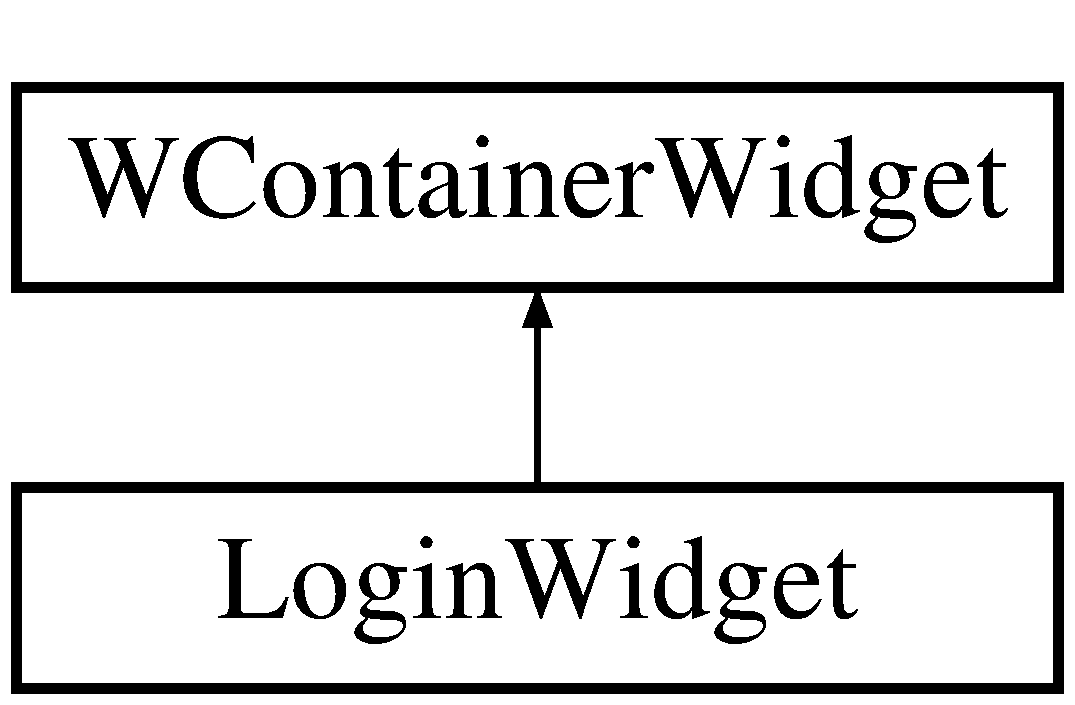
\includegraphics[height=2.000000cm]{classLoginWidget}
\end{center}
\end{figure}
\subsection*{Public Member Functions}
\begin{DoxyCompactItemize}
\item 
\hyperlink{classLoginWidget_a52aff5acb69d4510b807a583ec03bfec}{Login\+Widget} (Wt\+::\+W\+Container\+Widget $\ast$parent=0, \hyperlink{classAccount}{Account} $\ast$account=0, \hyperlink{classWelcomeScreen}{Welcome\+Screen} $\ast$main=0)
\begin{DoxyCompactList}\small\item\em Login Widget constructor. \end{DoxyCompactList}\item 
void \hyperlink{classLoginWidget_acc7476881ad942e634beafdeb4bdb971}{update} ()
\begin{DoxyCompactList}\small\item\em Update function, clears the widget and re-\/populates with elements of the login screen. \end{DoxyCompactList}\end{DoxyCompactItemize}
\subsection*{Private Member Functions}
\begin{DoxyCompactItemize}
\item 
void \hyperlink{classLoginWidget_af42b318f75370fd66e74c400bae44a4d}{submit} ()\hypertarget{classLoginWidget_af42b318f75370fd66e74c400bae44a4d}{}\label{classLoginWidget_af42b318f75370fd66e74c400bae44a4d}

\begin{DoxyCompactList}\small\item\em \hyperlink{classLoginWidget_af42b318f75370fd66e74c400bae44a4d}{submit()} function, triggered when user presses login button, displays any applicable warning messages and/or checks user database for authentication. Finally, it redirects to the bridge screen after successful login. \end{DoxyCompactList}\item 
bool \hyperlink{classLoginWidget_aa33a1ece55b698e9d5b8c91413715b36}{check\+Credentials} (std\+::string username, std\+::string password)
\begin{DoxyCompactList}\small\item\em \hyperlink{classLoginWidget_aa33a1ece55b698e9d5b8c91413715b36}{check\+Credentials()} function, checks for username.\+txt, then compares encrypted version of the user\textquotesingle{}s password \end{DoxyCompactList}\end{DoxyCompactItemize}
\subsection*{Private Attributes}
\begin{DoxyCompactItemize}
\item 
Wt\+::\+W\+Line\+Edit $\ast$ {\bfseries id\+Edit\+\_\+}\hypertarget{classLoginWidget_abc73734457aad449ae29568968397304}{}\label{classLoginWidget_abc73734457aad449ae29568968397304}

\item 
Wt\+::\+W\+Line\+Edit $\ast$ {\bfseries pw\+Edit\+\_\+}\hypertarget{classLoginWidget_aa1b7c49a9d9a3d742f1a8f6a35c2071c}{}\label{classLoginWidget_aa1b7c49a9d9a3d742f1a8f6a35c2071c}

\item 
Wt\+::\+W\+Push\+Button $\ast$ {\bfseries login\+Button\+\_\+}\hypertarget{classLoginWidget_aa4b647e9a3ef1beea1695b4ba4a072d2}{}\label{classLoginWidget_aa4b647e9a3ef1beea1695b4ba4a072d2}

\item 
Wt\+::\+W\+Text $\ast$ {\bfseries status\+Message\+\_\+}\hypertarget{classLoginWidget_adb0cb4c69680f0210583b7b1cabc3f25}{}\label{classLoginWidget_adb0cb4c69680f0210583b7b1cabc3f25}

\item 
Wt\+::\+W\+Reg\+Exp\+Validator $\ast$ {\bfseries username\+Validator\+\_\+}\hypertarget{classLoginWidget_a3f2aa506217f54e466fb3954cfb77a12}{}\label{classLoginWidget_a3f2aa506217f54e466fb3954cfb77a12}

\item 
Wt\+::\+W\+Length\+Validator $\ast$ {\bfseries password\+Length\+Validator\+\_\+}\hypertarget{classLoginWidget_a524d5c1e4c3cb20d050ce272cdfac23e}{}\label{classLoginWidget_a524d5c1e4c3cb20d050ce272cdfac23e}

\item 
\hyperlink{classWelcomeScreen}{Welcome\+Screen} $\ast$ {\bfseries parent\+\_\+}\hypertarget{classLoginWidget_a29e3645e6f24bcf909ba28665cd3663c}{}\label{classLoginWidget_a29e3645e6f24bcf909ba28665cd3663c}

\item 
\hyperlink{classAccount}{Account} $\ast$ {\bfseries account\+\_\+}\hypertarget{classLoginWidget_ac4303f10fd4fcd7a6ff43dae796f90e7}{}\label{classLoginWidget_ac4303f10fd4fcd7a6ff43dae796f90e7}

\end{DoxyCompactItemize}


\subsection{Constructor \& Destructor Documentation}
\index{Login\+Widget@{Login\+Widget}!Login\+Widget@{Login\+Widget}}
\index{Login\+Widget@{Login\+Widget}!Login\+Widget@{Login\+Widget}}
\subsubsection[{\texorpdfstring{Login\+Widget(\+Wt\+::\+W\+Container\+Widget $\ast$parent=0, Account $\ast$account=0, Welcome\+Screen $\ast$main=0)}{LoginWidget(Wt::WContainerWidget *parent=0, Account *account=0, WelcomeScreen *main=0)}}]{\setlength{\rightskip}{0pt plus 5cm}Login\+Widget\+::\+Login\+Widget (
\begin{DoxyParamCaption}
\item[{Wt\+::\+W\+Container\+Widget $\ast$}]{parent = {\ttfamily 0}, }
\item[{{\bf Account} $\ast$}]{account = {\ttfamily 0}, }
\item[{{\bf Welcome\+Screen} $\ast$}]{main = {\ttfamily 0}}
\end{DoxyParamCaption}
)}\hypertarget{classLoginWidget_a52aff5acb69d4510b807a583ec03bfec}{}\label{classLoginWidget_a52aff5acb69d4510b807a583ec03bfec}


Login Widget constructor. 


\begin{DoxyParams}{Parameters}
{\em $\ast$parent} & is a pointer the the containerwidget that stores this widget \\
\hline
{\em $\ast$account} & is a pointer to the user account object \\
\hline
{\em $\ast$main} & is a pointer to the app\textquotesingle{}s welcome screen \\
\hline
\end{DoxyParams}


\subsection{Member Function Documentation}
\index{Login\+Widget@{Login\+Widget}!check\+Credentials@{check\+Credentials}}
\index{check\+Credentials@{check\+Credentials}!Login\+Widget@{Login\+Widget}}
\subsubsection[{\texorpdfstring{check\+Credentials(std\+::string username, std\+::string password)}{checkCredentials(std::string username, std::string password)}}]{\setlength{\rightskip}{0pt plus 5cm}bool Login\+Widget\+::check\+Credentials (
\begin{DoxyParamCaption}
\item[{std\+::string}]{username, }
\item[{std\+::string}]{password}
\end{DoxyParamCaption}
)\hspace{0.3cm}{\ttfamily [private]}}\hypertarget{classLoginWidget_aa33a1ece55b698e9d5b8c91413715b36}{}\label{classLoginWidget_aa33a1ece55b698e9d5b8c91413715b36}


\hyperlink{classLoginWidget_aa33a1ece55b698e9d5b8c91413715b36}{check\+Credentials()} function, checks for username.\+txt, then compares encrypted version of the user\textquotesingle{}s password 


\begin{DoxyParams}{Parameters}
{\em username} & is a string representing the user\textquotesingle{}s inputted username \\
\hline
{\em password} & is a string representing the user\textquotesingle{}s inputted password \\
\hline
\end{DoxyParams}
\begin{DoxyReturn}{Returns}
bool representing if login successful 
\end{DoxyReturn}
\index{Login\+Widget@{Login\+Widget}!update@{update}}
\index{update@{update}!Login\+Widget@{Login\+Widget}}
\subsubsection[{\texorpdfstring{update()}{update()}}]{\setlength{\rightskip}{0pt plus 5cm}void Login\+Widget\+::update (
\begin{DoxyParamCaption}
{}
\end{DoxyParamCaption}
)}\hypertarget{classLoginWidget_acc7476881ad942e634beafdeb4bdb971}{}\label{classLoginWidget_acc7476881ad942e634beafdeb4bdb971}


Update function, clears the widget and re-\/populates with elements of the login screen. 

\begin{DoxyReturn}{Returns}
void 
\end{DoxyReturn}


The documentation for this class was generated from the following files\+:\begin{DoxyCompactItemize}
\item 
include/Login\+Widget.\+h\item 
src/\hyperlink{LoginWidget_8cpp}{Login\+Widget.\+cpp}\end{DoxyCompactItemize}

\hypertarget{classProfileWidget}{}\section{Profile\+Widget Class Reference}
\label{classProfileWidget}\index{Profile\+Widget@{Profile\+Widget}}
Inheritance diagram for Profile\+Widget\+:\begin{figure}[H]
\begin{center}
\leavevmode
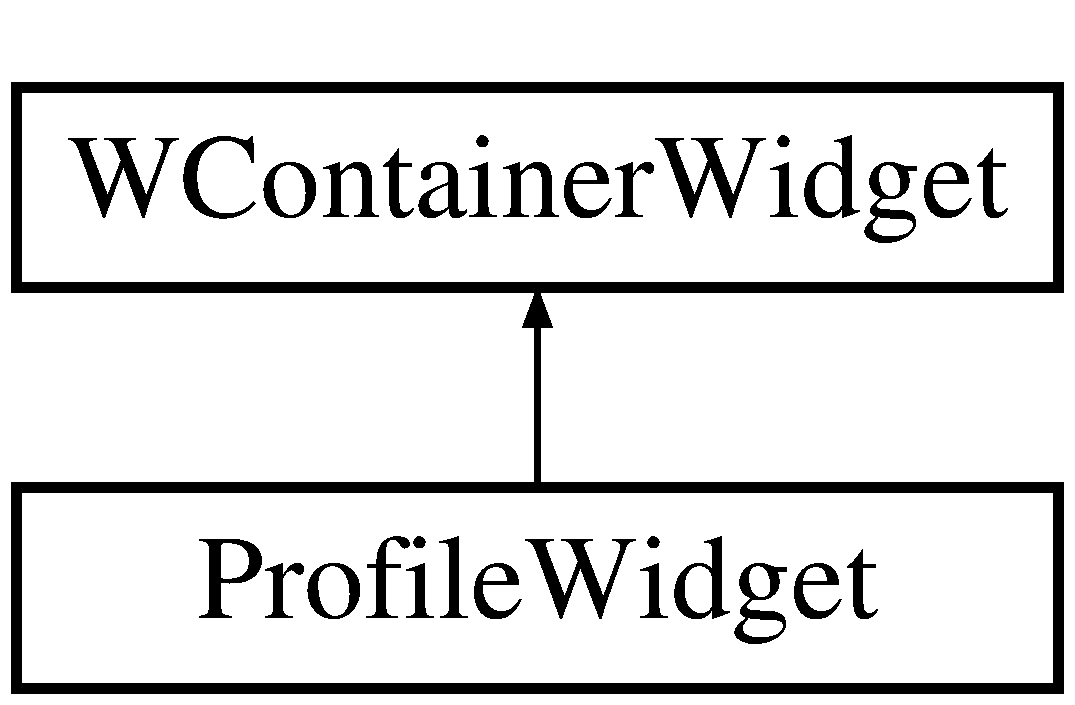
\includegraphics[height=2.000000cm]{classProfileWidget}
\end{center}
\end{figure}
\subsection*{Public Member Functions}
\begin{DoxyCompactItemize}
\item 
\hyperlink{classProfileWidget_a2fcfd867268b4ca8d3d8db067ad770df}{Profile\+Widget} (Wt\+::\+W\+Container\+Widget $\ast$parent=0, \hyperlink{classAccount}{Account} $\ast$account=0, \hyperlink{classWelcomeScreen}{Welcome\+Screen} $\ast$main=0)
\begin{DoxyCompactList}\small\item\em Profile Widget constructor. \end{DoxyCompactList}\item 
void \hyperlink{classProfileWidget_a6c093ffd95dedf4814b10b53865784ca}{update} ()
\begin{DoxyCompactList}\small\item\em Update function, clears the widget and re-\/populates with elements of the profile screen. \end{DoxyCompactList}\end{DoxyCompactItemize}
\subsection*{Private Member Functions}
\begin{DoxyCompactItemize}
\item 
void \hyperlink{classProfileWidget_a07bcf16818fe49254c5aa80eefdc68b8}{update\+First\+Name} ()
\begin{DoxyCompactList}\small\item\em update\+First\+Name function, called if user puts in a new first name, calls the setter function of \hyperlink{classAccount}{Account} screen \end{DoxyCompactList}\item 
void \hyperlink{classProfileWidget_a990300c69c3177fea08ae6af21d33945}{update\+Last\+Name} ()
\begin{DoxyCompactList}\small\item\em update\+Last\+Name function, called if user puts in a new last name, calls the setter function of \hyperlink{classAccount}{Account} screen \end{DoxyCompactList}\item 
void \hyperlink{classProfileWidget_a9dff9212fcc936cc5a77db50b3675adb}{show\+Password\+Dialog} ()
\begin{DoxyCompactList}\small\item\em show\+Password\+Dialog function, called if user chooses to update their password. Opens a W\+Dialog box asking them to confirm their current password, and choose a new password, goes through same validation process as the create account page \end{DoxyCompactList}\item 
bool \hyperlink{classProfileWidget_a68729c760462780f9b1bf5e9dac739db}{check\+Valid\+Password} (std\+::string pass)
\begin{DoxyCompactList}\small\item\em check\+Valid\+Password function, ensures that the password that the user has entered is the password connected to their account \end{DoxyCompactList}\item 
void \hyperlink{classProfileWidget_a0b822b0db6c6e3194d61b5cd427dff64}{update\+Password} ()
\begin{DoxyCompactList}\small\item\em update\+Password function, called upon submission of the update password dialog box. Validates password and sets the \hyperlink{classAccount}{Account}\textquotesingle{}s new password using \hyperlink{classAccount}{Account} setter \end{DoxyCompactList}\item 
void \hyperlink{classProfileWidget_a1e6942fd023d790cc5c2bcb26fa5a745}{upload\+Profile\+Picture} (std\+::string file)
\begin{DoxyCompactList}\small\item\em upload\+Profile\+Picture function, called if user uploads a profile picture, saves the file in a non-\/temporary location \end{DoxyCompactList}\end{DoxyCompactItemize}
\subsection*{Private Attributes}
\begin{DoxyCompactItemize}
\item 
\hyperlink{classWelcomeScreen}{Welcome\+Screen} $\ast$ {\bfseries parent\+\_\+}\hypertarget{classProfileWidget_a56c218a697d3523f5a531ad035d927ed}{}\label{classProfileWidget_a56c218a697d3523f5a531ad035d927ed}

\item 
\hyperlink{classAccount}{Account} $\ast$ {\bfseries account\+\_\+}\hypertarget{classProfileWidget_aecefc74b58e1451e684636ba036a6f2f}{}\label{classProfileWidget_aecefc74b58e1451e684636ba036a6f2f}

\item 
Wt\+::\+W\+In\+Place\+Edit $\ast$ {\bfseries editable\+First\+Name\+\_\+}\hypertarget{classProfileWidget_a2b69c8124758bad87a3fbf02eeaa040b}{}\label{classProfileWidget_a2b69c8124758bad87a3fbf02eeaa040b}

\item 
Wt\+::\+W\+In\+Place\+Edit $\ast$ {\bfseries editable\+Last\+Name\+\_\+}\hypertarget{classProfileWidget_a5df00d4c05fd6ed97e633480507c17db}{}\label{classProfileWidget_a5df00d4c05fd6ed97e633480507c17db}

\item 
Wt\+::\+W\+Push\+Button $\ast$ {\bfseries update\+Password\+\_\+}\hypertarget{classProfileWidget_a6bee4c694aa7feae407acaa78288746c}{}\label{classProfileWidget_a6bee4c694aa7feae407acaa78288746c}

\item 
Wt\+::\+W\+Dialog $\ast$ {\bfseries password\+Dialog\+\_\+}\hypertarget{classProfileWidget_aec70048f76904c94c7d20cf9a60f5ad6}{}\label{classProfileWidget_aec70048f76904c94c7d20cf9a60f5ad6}

\item 
Wt\+::\+W\+Line\+Edit $\ast$ {\bfseries current\+Pass\+\_\+}\hypertarget{classProfileWidget_a6c15ca5e77a019a4c9ec63c6065dc669}{}\label{classProfileWidget_a6c15ca5e77a019a4c9ec63c6065dc669}

\item 
Wt\+::\+W\+Line\+Edit $\ast$ {\bfseries new\+Pass\+\_\+}\hypertarget{classProfileWidget_ae672f881b80a6f14f05cff1429faf609}{}\label{classProfileWidget_ae672f881b80a6f14f05cff1429faf609}

\item 
Wt\+::\+W\+Line\+Edit $\ast$ {\bfseries confirm\+New\+Pass\+\_\+}\hypertarget{classProfileWidget_a30033dd6bf1ea9dacb4e51e91f5a6286}{}\label{classProfileWidget_a30033dd6bf1ea9dacb4e51e91f5a6286}

\item 
Wt\+::\+W\+Text $\ast$ {\bfseries password\+Error\+\_\+}\hypertarget{classProfileWidget_abcac84401d90ac8447f3cb11951cbd76}{}\label{classProfileWidget_abcac84401d90ac8447f3cb11951cbd76}

\item 
Wt\+::\+W\+Text $\ast$ {\bfseries password\+Success\+\_\+}\hypertarget{classProfileWidget_a83350d03805517f9564bada67140d4f6}{}\label{classProfileWidget_a83350d03805517f9564bada67140d4f6}

\item 
Wt\+::\+W\+File\+Upload $\ast$ {\bfseries pic\+Upload\+\_\+}\hypertarget{classProfileWidget_a3297479e7efd5b09b1bdda6251ec08aa}{}\label{classProfileWidget_a3297479e7efd5b09b1bdda6251ec08aa}

\item 
Wt\+::\+W\+Text $\ast$ {\bfseries profile\+Pic\+Out\+Message\+\_\+}\hypertarget{classProfileWidget_afc047a157b120548478c90899668d6ba}{}\label{classProfileWidget_afc047a157b120548478c90899668d6ba}

\item 
bool {\bfseries file\+Too\+Large} = false\hypertarget{classProfileWidget_a1349cc67751fd8b5cbb6f0256fda652d}{}\label{classProfileWidget_a1349cc67751fd8b5cbb6f0256fda652d}

\item 
Wt\+::\+W\+Validator $\ast$ {\bfseries input\+Not\+Empty\+\_\+}\hypertarget{classProfileWidget_acef4ab69bb13e9c505e564aa82b1bc52}{}\label{classProfileWidget_acef4ab69bb13e9c505e564aa82b1bc52}

\item 
Wt\+::\+W\+Length\+Validator $\ast$ {\bfseries password\+Length\+Validator\+\_\+}\hypertarget{classProfileWidget_aaa2506199f35edd1dd02389b020da70f}{}\label{classProfileWidget_aaa2506199f35edd1dd02389b020da70f}

\end{DoxyCompactItemize}


\subsection{Constructor \& Destructor Documentation}
\index{Profile\+Widget@{Profile\+Widget}!Profile\+Widget@{Profile\+Widget}}
\index{Profile\+Widget@{Profile\+Widget}!Profile\+Widget@{Profile\+Widget}}
\subsubsection[{\texorpdfstring{Profile\+Widget(\+Wt\+::\+W\+Container\+Widget $\ast$parent=0, Account $\ast$account=0, Welcome\+Screen $\ast$main=0)}{ProfileWidget(Wt::WContainerWidget *parent=0, Account *account=0, WelcomeScreen *main=0)}}]{\setlength{\rightskip}{0pt plus 5cm}Profile\+Widget\+::\+Profile\+Widget (
\begin{DoxyParamCaption}
\item[{Wt\+::\+W\+Container\+Widget $\ast$}]{parent = {\ttfamily 0}, }
\item[{{\bf Account} $\ast$}]{account = {\ttfamily 0}, }
\item[{{\bf Welcome\+Screen} $\ast$}]{main = {\ttfamily 0}}
\end{DoxyParamCaption}
)}\hypertarget{classProfileWidget_a2fcfd867268b4ca8d3d8db067ad770df}{}\label{classProfileWidget_a2fcfd867268b4ca8d3d8db067ad770df}


Profile Widget constructor. 


\begin{DoxyParams}{Parameters}
{\em $\ast$parent} & is a pointer the the containerwidget that stores this widget \\
\hline
{\em $\ast$main} & is a pointer to the app\textquotesingle{}s welcome screen \\
\hline
\end{DoxyParams}


\subsection{Member Function Documentation}
\index{Profile\+Widget@{Profile\+Widget}!check\+Valid\+Password@{check\+Valid\+Password}}
\index{check\+Valid\+Password@{check\+Valid\+Password}!Profile\+Widget@{Profile\+Widget}}
\subsubsection[{\texorpdfstring{check\+Valid\+Password(std\+::string pass)}{checkValidPassword(std::string pass)}}]{\setlength{\rightskip}{0pt plus 5cm}bool Profile\+Widget\+::check\+Valid\+Password (
\begin{DoxyParamCaption}
\item[{std\+::string}]{pass}
\end{DoxyParamCaption}
)\hspace{0.3cm}{\ttfamily [private]}}\hypertarget{classProfileWidget_a68729c760462780f9b1bf5e9dac739db}{}\label{classProfileWidget_a68729c760462780f9b1bf5e9dac739db}


check\+Valid\+Password function, ensures that the password that the user has entered is the password connected to their account 

\begin{DoxyReturn}{Returns}
bool true if the password is correct, false otherwise 
\end{DoxyReturn}
\index{Profile\+Widget@{Profile\+Widget}!show\+Password\+Dialog@{show\+Password\+Dialog}}
\index{show\+Password\+Dialog@{show\+Password\+Dialog}!Profile\+Widget@{Profile\+Widget}}
\subsubsection[{\texorpdfstring{show\+Password\+Dialog()}{showPasswordDialog()}}]{\setlength{\rightskip}{0pt plus 5cm}void Profile\+Widget\+::show\+Password\+Dialog (
\begin{DoxyParamCaption}
{}
\end{DoxyParamCaption}
)\hspace{0.3cm}{\ttfamily [private]}}\hypertarget{classProfileWidget_a9dff9212fcc936cc5a77db50b3675adb}{}\label{classProfileWidget_a9dff9212fcc936cc5a77db50b3675adb}


show\+Password\+Dialog function, called if user chooses to update their password. Opens a W\+Dialog box asking them to confirm their current password, and choose a new password, goes through same validation process as the create account page 

\begin{DoxyReturn}{Returns}
void 
\end{DoxyReturn}
\index{Profile\+Widget@{Profile\+Widget}!update@{update}}
\index{update@{update}!Profile\+Widget@{Profile\+Widget}}
\subsubsection[{\texorpdfstring{update()}{update()}}]{\setlength{\rightskip}{0pt plus 5cm}void Profile\+Widget\+::update (
\begin{DoxyParamCaption}
{}
\end{DoxyParamCaption}
)}\hypertarget{classProfileWidget_a6c093ffd95dedf4814b10b53865784ca}{}\label{classProfileWidget_a6c093ffd95dedf4814b10b53865784ca}


Update function, clears the widget and re-\/populates with elements of the profile screen. 

\begin{DoxyReturn}{Returns}
void 
\end{DoxyReturn}
\index{Profile\+Widget@{Profile\+Widget}!update\+First\+Name@{update\+First\+Name}}
\index{update\+First\+Name@{update\+First\+Name}!Profile\+Widget@{Profile\+Widget}}
\subsubsection[{\texorpdfstring{update\+First\+Name()}{updateFirstName()}}]{\setlength{\rightskip}{0pt plus 5cm}void Profile\+Widget\+::update\+First\+Name (
\begin{DoxyParamCaption}
{}
\end{DoxyParamCaption}
)\hspace{0.3cm}{\ttfamily [private]}}\hypertarget{classProfileWidget_a07bcf16818fe49254c5aa80eefdc68b8}{}\label{classProfileWidget_a07bcf16818fe49254c5aa80eefdc68b8}


update\+First\+Name function, called if user puts in a new first name, calls the setter function of \hyperlink{classAccount}{Account} screen 

\begin{DoxyReturn}{Returns}
void 
\end{DoxyReturn}
\index{Profile\+Widget@{Profile\+Widget}!update\+Last\+Name@{update\+Last\+Name}}
\index{update\+Last\+Name@{update\+Last\+Name}!Profile\+Widget@{Profile\+Widget}}
\subsubsection[{\texorpdfstring{update\+Last\+Name()}{updateLastName()}}]{\setlength{\rightskip}{0pt plus 5cm}void Profile\+Widget\+::update\+Last\+Name (
\begin{DoxyParamCaption}
{}
\end{DoxyParamCaption}
)\hspace{0.3cm}{\ttfamily [private]}}\hypertarget{classProfileWidget_a990300c69c3177fea08ae6af21d33945}{}\label{classProfileWidget_a990300c69c3177fea08ae6af21d33945}


update\+Last\+Name function, called if user puts in a new last name, calls the setter function of \hyperlink{classAccount}{Account} screen 

\begin{DoxyReturn}{Returns}
void 
\end{DoxyReturn}
\index{Profile\+Widget@{Profile\+Widget}!update\+Password@{update\+Password}}
\index{update\+Password@{update\+Password}!Profile\+Widget@{Profile\+Widget}}
\subsubsection[{\texorpdfstring{update\+Password()}{updatePassword()}}]{\setlength{\rightskip}{0pt plus 5cm}void Profile\+Widget\+::update\+Password (
\begin{DoxyParamCaption}
{}
\end{DoxyParamCaption}
)\hspace{0.3cm}{\ttfamily [private]}}\hypertarget{classProfileWidget_a0b822b0db6c6e3194d61b5cd427dff64}{}\label{classProfileWidget_a0b822b0db6c6e3194d61b5cd427dff64}


update\+Password function, called upon submission of the update password dialog box. Validates password and sets the \hyperlink{classAccount}{Account}\textquotesingle{}s new password using \hyperlink{classAccount}{Account} setter 

\begin{DoxyReturn}{Returns}
void 
\end{DoxyReturn}
\index{Profile\+Widget@{Profile\+Widget}!upload\+Profile\+Picture@{upload\+Profile\+Picture}}
\index{upload\+Profile\+Picture@{upload\+Profile\+Picture}!Profile\+Widget@{Profile\+Widget}}
\subsubsection[{\texorpdfstring{upload\+Profile\+Picture(std\+::string file)}{uploadProfilePicture(std::string file)}}]{\setlength{\rightskip}{0pt plus 5cm}void Profile\+Widget\+::upload\+Profile\+Picture (
\begin{DoxyParamCaption}
\item[{std\+::string}]{file}
\end{DoxyParamCaption}
)\hspace{0.3cm}{\ttfamily [private]}}\hypertarget{classProfileWidget_a1e6942fd023d790cc5c2bcb26fa5a745}{}\label{classProfileWidget_a1e6942fd023d790cc5c2bcb26fa5a745}


upload\+Profile\+Picture function, called if user uploads a profile picture, saves the file in a non-\/temporary location 


\begin{DoxyParams}{Parameters}
{\em location} & of the temporary file location\\
\hline
\end{DoxyParams}
\begin{DoxyReturn}{Returns}
void 
\end{DoxyReturn}


The documentation for this class was generated from the following files\+:\begin{DoxyCompactItemize}
\item 
include/Profile\+Widget.\+h\item 
src/\hyperlink{ProfileWidget_8cpp}{Profile\+Widget.\+cpp}\end{DoxyCompactItemize}

\hypertarget{structrgb}{}\section{rgb Struct Reference}
\label{structrgb}\index{rgb@{rgb}}
\subsection*{Public Attributes}
\begin{DoxyCompactItemize}
\item 
float {\bfseries r}\hypertarget{structrgb_a417987de6545982be6012a0c8ba517c6}{}\label{structrgb_a417987de6545982be6012a0c8ba517c6}

\item 
float {\bfseries g}\hypertarget{structrgb_a8ebc8e4a87db5d5dda3980b88fe31f35}{}\label{structrgb_a8ebc8e4a87db5d5dda3980b88fe31f35}

\item 
float {\bfseries b}\hypertarget{structrgb_ac2be2182f82e2c3c99860a560b19ec57}{}\label{structrgb_ac2be2182f82e2c3c99860a560b19ec57}

\item 
float {\bfseries brightness}\hypertarget{structrgb_a7ce9332d007827250f0c693403dc95e0}{}\label{structrgb_a7ce9332d007827250f0c693403dc95e0}

\end{DoxyCompactItemize}


The documentation for this struct was generated from the following files\+:\begin{DoxyCompactItemize}
\item 
include/Colour\+Convert.\+h\item 
include/Hash.\+h\end{DoxyCompactItemize}

\hypertarget{classSchedule}{}\section{Schedule Class Reference}
\label{classSchedule}\index{Schedule@{Schedule}}
\subsection*{Public Member Functions}
\begin{DoxyCompactItemize}
\item 
\hyperlink{classSchedule_afe65128cb206d7e0229f605e1c90da87}{Schedule} (W\+String schedule\+Num, Json\+::\+Object schedule\+Data)
\begin{DoxyCompactList}\small\item\em \hyperlink{classSchedule}{Schedule} constructor. \end{DoxyCompactList}\item 
virtual \hyperlink{classSchedule_a4806b985197d35c00b9e707c0ed87998}{$\sim$\+Schedule} ()\hypertarget{classSchedule_a4806b985197d35c00b9e707c0ed87998}{}\label{classSchedule_a4806b985197d35c00b9e707c0ed87998}

\begin{DoxyCompactList}\small\item\em \hyperlink{classSchedule}{Schedule} destructor. \end{DoxyCompactList}\item 
W\+String {\bfseries get\+Schedulenum} ()\hypertarget{classSchedule_af95608a4e73b38a6bcf80f36d351013b}{}\label{classSchedule_af95608a4e73b38a6bcf80f36d351013b}

\item 
W\+String {\bfseries get\+Name} ()\hypertarget{classSchedule_a69ae9ed980b215b71de84c4290518ff9}{}\label{classSchedule_a69ae9ed980b215b71de84c4290518ff9}

\item 
W\+String {\bfseries get\+Description} ()\hypertarget{classSchedule_abfb0f1e5facf1f66b020cfea5950a37d}{}\label{classSchedule_abfb0f1e5facf1f66b020cfea5950a37d}

\item 
W\+String {\bfseries get\+Time} ()\hypertarget{classSchedule_a386615e99bce9e7cb09a7644d73a13a5}{}\label{classSchedule_a386615e99bce9e7cb09a7644d73a13a5}

\item 
W\+String {\bfseries get\+Address} ()\hypertarget{classSchedule_a6dddd11e63ea56b3d26ee85ca25005c9}{}\label{classSchedule_a6dddd11e63ea56b3d26ee85ca25005c9}

\item 
W\+String {\bfseries get\+Method} ()\hypertarget{classSchedule_a2ae454af806b7267638604708d56c30d}{}\label{classSchedule_a2ae454af806b7267638604708d56c30d}

\item 
int {\bfseries get\+Bri} ()\hypertarget{classSchedule_a523887b9f605ac61d889f37992e1ce5d}{}\label{classSchedule_a523887b9f605ac61d889f37992e1ce5d}

\item 
int {\bfseries get\+Transition} ()\hypertarget{classSchedule_ab7dd20460a37285ff148793d53bd3009}{}\label{classSchedule_ab7dd20460a37285ff148793d53bd3009}

\item 
bool {\bfseries get\+On} ()\hypertarget{classSchedule_a79f7d6614861bf32a74c39534b6d0950}{}\label{classSchedule_a79f7d6614861bf32a74c39534b6d0950}

\item 
double {\bfseries getX} ()\hypertarget{classSchedule_aae6f22f411115261a90ceac1898555fc}{}\label{classSchedule_aae6f22f411115261a90ceac1898555fc}

\item 
double {\bfseries getY} ()\hypertarget{classSchedule_a83264d6f96c0b80a8983f178a80ef859}{}\label{classSchedule_a83264d6f96c0b80a8983f178a80ef859}

\end{DoxyCompactItemize}
\subsection*{Private Attributes}
\begin{DoxyCompactItemize}
\item 
W\+String {\bfseries schedulenum\+\_\+}\hypertarget{classSchedule_a005bb3a882562c4372e39a358c36ca7e}{}\label{classSchedule_a005bb3a882562c4372e39a358c36ca7e}

\item 
W\+String {\bfseries name\+\_\+}\hypertarget{classSchedule_a25b69fcd31d166f58d67a75d60ac9577}{}\label{classSchedule_a25b69fcd31d166f58d67a75d60ac9577}

\item 
W\+String {\bfseries description\+\_\+}\hypertarget{classSchedule_ae03217757e3008251f9a95d05498f03b}{}\label{classSchedule_ae03217757e3008251f9a95d05498f03b}

\item 
W\+String {\bfseries time\+\_\+}\hypertarget{classSchedule_ae00d1743e41733136886991206ffff2f}{}\label{classSchedule_ae00d1743e41733136886991206ffff2f}

\item 
W\+String {\bfseries address\+\_\+}\hypertarget{classSchedule_a2f57981c1518ccec1d01029f420f7e52}{}\label{classSchedule_a2f57981c1518ccec1d01029f420f7e52}

\item 
W\+String {\bfseries method\+\_\+}\hypertarget{classSchedule_a1c5984e5e2af62e9d7fa102145b1dc25}{}\label{classSchedule_a1c5984e5e2af62e9d7fa102145b1dc25}

\item 
int {\bfseries bri\+\_\+}\hypertarget{classSchedule_ae9d5056689f601884d77975dc30675ac}{}\label{classSchedule_ae9d5056689f601884d77975dc30675ac}

\item 
int {\bfseries transition\+\_\+}\hypertarget{classSchedule_a69ab0f52f52a36e56deb742e0a6e34ab}{}\label{classSchedule_a69ab0f52f52a36e56deb742e0a6e34ab}

\item 
bool {\bfseries on\+\_\+}\hypertarget{classSchedule_a719dfbf299545d78448a969acd24ae0a}{}\label{classSchedule_a719dfbf299545d78448a969acd24ae0a}

\item 
vector$<$ double $>$ {\bfseries xy\+\_\+}\hypertarget{classSchedule_aa07cbad9b0c2d089d233036567063032}{}\label{classSchedule_aa07cbad9b0c2d089d233036567063032}

\end{DoxyCompactItemize}


\subsection{Constructor \& Destructor Documentation}
\index{Schedule@{Schedule}!Schedule@{Schedule}}
\index{Schedule@{Schedule}!Schedule@{Schedule}}
\subsubsection[{\texorpdfstring{Schedule(\+W\+String schedule\+Num, Json\+::\+Object schedule\+Data)}{Schedule(WString scheduleNum, Json::Object scheduleData)}}]{\setlength{\rightskip}{0pt plus 5cm}Schedule\+::\+Schedule (
\begin{DoxyParamCaption}
\item[{W\+String}]{schedule\+Num, }
\item[{Json\+::\+Object}]{schedule\+Data}
\end{DoxyParamCaption}
)}\hypertarget{classSchedule_afe65128cb206d7e0229f605e1c90da87}{}\label{classSchedule_afe65128cb206d7e0229f605e1c90da87}


\hyperlink{classSchedule}{Schedule} constructor. 


\begin{DoxyParams}{Parameters}
{\em schedule\+Num} & the number key for the \hyperlink{classSchedule}{Schedule} in the Hue A\+PI \\
\hline
{\em schedule\+Data} & the Json object of a \hyperlink{classSchedule}{Schedule} from the Hue A\+PI \\
\hline
\end{DoxyParams}


The documentation for this class was generated from the following files\+:\begin{DoxyCompactItemize}
\item 
include/Schedule.\+h\item 
src/\hyperlink{Schedule_8cpp}{Schedule.\+cpp}\end{DoxyCompactItemize}

\hypertarget{classWelcomeScreen}{}\section{Welcome\+Screen Class Reference}
\label{classWelcomeScreen}\index{Welcome\+Screen@{Welcome\+Screen}}
Inheritance diagram for Welcome\+Screen\+:\begin{figure}[H]
\begin{center}
\leavevmode
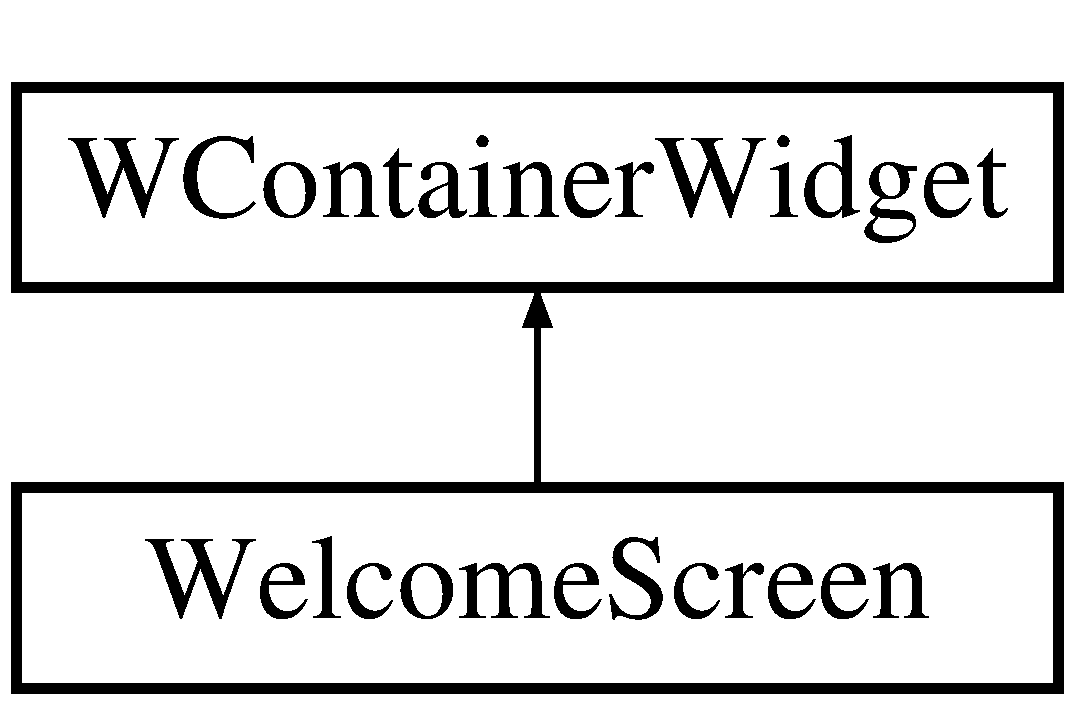
\includegraphics[height=2.000000cm]{classWelcomeScreen}
\end{center}
\end{figure}
\subsection*{Public Member Functions}
\begin{DoxyCompactItemize}
\item 
\hyperlink{classWelcomeScreen_a9d614d7c0a65f5f161fdd62016cccb02}{Welcome\+Screen} (Wt\+::\+W\+Container\+Widget $\ast$parent=0)
\begin{DoxyCompactList}\small\item\em Main Screen constructor. \end{DoxyCompactList}\item 
void \hyperlink{classWelcomeScreen_a7301f3941c1ff0caa7045329c71c41a7}{handle\+Internal\+Path} (const std\+::string \&internal\+Path)
\begin{DoxyCompactList}\small\item\em Handle Internal Path function, checks for any changes to the internal path and redirects the page according to internal\+Path. \end{DoxyCompactList}\item 
\hyperlink{classAccount}{Account} {\bfseries get\+Account} ()\hypertarget{classWelcomeScreen_a4cd28472ee9233a9f4d32d4804163e79}{}\label{classWelcomeScreen_a4cd28472ee9233a9f4d32d4804163e79}

\item 
void {\bfseries set\+Account} (\hyperlink{classAccount}{Account} account)\hypertarget{classWelcomeScreen_a087ed7ee3186e47863edb316fba2512d}{}\label{classWelcomeScreen_a087ed7ee3186e47863edb316fba2512d}

\item 
void {\bfseries connect\+Bridge} ()\hypertarget{classWelcomeScreen_a5b212d7e956e08f9a4cfb6ea509e65cc}{}\label{classWelcomeScreen_a5b212d7e956e08f9a4cfb6ea509e65cc}

\item 
void {\bfseries handle\+Http\+Response} (boost\+::system\+::error\+\_\+code err, const Wt\+::\+Http\+::\+Message \&response)\hypertarget{classWelcomeScreen_a83e9eafc251ce2b4e1e844a218aa3a1a}{}\label{classWelcomeScreen_a83e9eafc251ce2b4e1e844a218aa3a1a}

\item 
void \hyperlink{classWelcomeScreen_afd5f059dbc60e31015b1f210f6bc16e0}{update\+Profile\+Name} ()
\begin{DoxyCompactList}\small\item\em Updates name of logged in user on the top menu bar. \end{DoxyCompactList}\item 
void \hyperlink{classWelcomeScreen_abe56adce06150723d19ae52713f4b8cc}{login\+Success} ()
\begin{DoxyCompactList}\small\item\em Validates user account to logged in after successful login. \end{DoxyCompactList}\end{DoxyCompactItemize}
\subsection*{Private Member Functions}
\begin{DoxyCompactItemize}
\item 
void \hyperlink{classWelcomeScreen_a720c47b7f03f1423139e9a0f6a1693ba}{login\+Screen} ()
\begin{DoxyCompactList}\small\item\em Login screen function, updates the page to the login screen. \end{DoxyCompactList}\item 
void \hyperlink{classWelcomeScreen_ab61fd209d95cc39b46a9bc0526304264}{create\+Account\+Screen} ()
\begin{DoxyCompactList}\small\item\em Create \hyperlink{classAccount}{Account} function, updates the page to the creation screen. \end{DoxyCompactList}\item 
void \hyperlink{classWelcomeScreen_af1587d0a89a8daf995dd851b24daa8b1}{bridge\+Screen} ()
\begin{DoxyCompactList}\small\item\em \hyperlink{classBridge}{Bridge} function, updates the page to the bridge control screen. \end{DoxyCompactList}\item 
void \hyperlink{classWelcomeScreen_a8c16248993785198885cb22a82113f99}{profile\+Screen} ()
\begin{DoxyCompactList}\small\item\em profile screen function, updates the page to the profile management screen \end{DoxyCompactList}\item 
void \hyperlink{classWelcomeScreen_aecd7b015439dfb5bdbe86ed9d8c229fc}{light\+Management\+Screen} (int index)
\begin{DoxyCompactList}\small\item\em Creates a new \hyperlink{classLightManagementWidget}{Light\+Management\+Widget} for a \hyperlink{classBridge}{Bridge} in in the \hyperlink{classAccount}{Account} bridges vector at index. \end{DoxyCompactList}\end{DoxyCompactItemize}
\subsection*{Private Attributes}
\begin{DoxyCompactItemize}
\item 
Wt\+::\+W\+Navigation\+Bar $\ast$ {\bfseries nav\+Bar\+\_\+}\hypertarget{classWelcomeScreen_a4667ce16e321647494567feadd35d05c}{}\label{classWelcomeScreen_a4667ce16e321647494567feadd35d05c}

\item 
Wt\+::\+W\+Menu\+Item $\ast$ {\bfseries login\+Menu\+Item\+\_\+}\hypertarget{classWelcomeScreen_a6866061b373f0f60e644ce3ae0d8783a}{}\label{classWelcomeScreen_a6866061b373f0f60e644ce3ae0d8783a}

\item 
Wt\+::\+W\+Menu\+Item $\ast$ {\bfseries create\+Menu\+Item\+\_\+}\hypertarget{classWelcomeScreen_aa78bc9664decc36f6eb6e81d9bd6f62d}{}\label{classWelcomeScreen_aa78bc9664decc36f6eb6e81d9bd6f62d}

\item 
Wt\+::\+W\+Menu\+Item $\ast$ {\bfseries bridges\+Menu\+Item\+\_\+}\hypertarget{classWelcomeScreen_a33f154c6595ce305c06bad498ec993cb}{}\label{classWelcomeScreen_a33f154c6595ce305c06bad498ec993cb}

\item 
Wt\+::\+W\+Menu\+Item $\ast$ {\bfseries profile\+Menu\+Item\+\_\+}\hypertarget{classWelcomeScreen_a3ebebbe939515f59f78ed2af34523da2}{}\label{classWelcomeScreen_a3ebebbe939515f59f78ed2af34523da2}

\item 
Wt\+::\+W\+Menu\+Item $\ast$ {\bfseries logout\+Menu\+Item\+\_\+}\hypertarget{classWelcomeScreen_a6737befd56f21e10ea6426eee30c8943}{}\label{classWelcomeScreen_a6737befd56f21e10ea6426eee30c8943}

\item 
Wt\+::\+W\+Text $\ast$ {\bfseries server\+Message\+\_\+}\hypertarget{classWelcomeScreen_adf01c5bef52bb8f08dd2f6e973d06761}{}\label{classWelcomeScreen_adf01c5bef52bb8f08dd2f6e973d06761}

\item 
Wt\+::\+W\+Anchor $\ast$ {\bfseries profile\+Anchor\+\_\+}\hypertarget{classWelcomeScreen_ab307ac80202c76a641fe69c79b75e4c8}{}\label{classWelcomeScreen_ab307ac80202c76a641fe69c79b75e4c8}

\item 
Wt\+::\+W\+Anchor $\ast$ {\bfseries home\+Anchor\+\_\+}\hypertarget{classWelcomeScreen_a343ab978f9d097e2af07f92f3a09d979}{}\label{classWelcomeScreen_a343ab978f9d097e2af07f92f3a09d979}

\item 
Wt\+::\+W\+Stacked\+Widget $\ast$ {\bfseries main\+Stack\+\_\+}\hypertarget{classWelcomeScreen_aa6c17ce8f5bfd42984336cb3e2ac3463}{}\label{classWelcomeScreen_aa6c17ce8f5bfd42984336cb3e2ac3463}

\item 
Wt\+::\+W\+Container\+Widget $\ast$ {\bfseries links\+\_\+}\hypertarget{classWelcomeScreen_aea50aeb2ceeaa7046396a48dcbb12271}{}\label{classWelcomeScreen_aea50aeb2ceeaa7046396a48dcbb12271}

\item 
\hyperlink{classCreateAccountWidget}{Create\+Account\+Widget} $\ast$ {\bfseries create\+Screen\+\_\+}\hypertarget{classWelcomeScreen_a6957eca431d149cdc83febea171247fb}{}\label{classWelcomeScreen_a6957eca431d149cdc83febea171247fb}

\item 
\hyperlink{classLoginWidget}{Login\+Widget} $\ast$ {\bfseries login\+Screen\+\_\+}\hypertarget{classWelcomeScreen_a5be85a6336144771ac59e1ae10ac4711}{}\label{classWelcomeScreen_a5be85a6336144771ac59e1ae10ac4711}

\item 
\hyperlink{classBridgeScreenWidget}{Bridge\+Screen\+Widget} $\ast$ {\bfseries bridge\+Screen\+\_\+}\hypertarget{classWelcomeScreen_ab83d4d326b0205cf8e56dbe1b53055df}{}\label{classWelcomeScreen_ab83d4d326b0205cf8e56dbe1b53055df}

\item 
\hyperlink{classProfileWidget}{Profile\+Widget} $\ast$ {\bfseries profile\+Screen\+\_\+}\hypertarget{classWelcomeScreen_a018888199a71b1c16bcf16b1b49f2d73}{}\label{classWelcomeScreen_a018888199a71b1c16bcf16b1b49f2d73}

\item 
\hyperlink{classLightManagementWidget}{Light\+Management\+Widget} $\ast$ {\bfseries light\+Manage\+\_\+}\hypertarget{classWelcomeScreen_a4bd816f28e599ade3e31c90e9e5e7ea7}{}\label{classWelcomeScreen_a4bd816f28e599ade3e31c90e9e5e7ea7}

\item 
\hyperlink{classAccount}{Account} {\bfseries account\+\_\+}\hypertarget{classWelcomeScreen_a061965fc25cdc564b17ec23880a56e20}{}\label{classWelcomeScreen_a061965fc25cdc564b17ec23880a56e20}

\end{DoxyCompactItemize}


\subsection{Constructor \& Destructor Documentation}
\index{Welcome\+Screen@{Welcome\+Screen}!Welcome\+Screen@{Welcome\+Screen}}
\index{Welcome\+Screen@{Welcome\+Screen}!Welcome\+Screen@{Welcome\+Screen}}
\subsubsection[{\texorpdfstring{Welcome\+Screen(\+Wt\+::\+W\+Container\+Widget $\ast$parent=0)}{WelcomeScreen(Wt::WContainerWidget *parent=0)}}]{\setlength{\rightskip}{0pt plus 5cm}Welcome\+Screen\+::\+Welcome\+Screen (
\begin{DoxyParamCaption}
\item[{Wt\+::\+W\+Container\+Widget $\ast$}]{parent = {\ttfamily 0}}
\end{DoxyParamCaption}
)}\hypertarget{classWelcomeScreen_a9d614d7c0a65f5f161fdd62016cccb02}{}\label{classWelcomeScreen_a9d614d7c0a65f5f161fdd62016cccb02}


Main Screen constructor. 


\begin{DoxyParams}{Parameters}
{\em $\ast$parent} & is a pointer the the containerwidget that stores this widget \\
\hline
\end{DoxyParams}


\subsection{Member Function Documentation}
\index{Welcome\+Screen@{Welcome\+Screen}!bridge\+Screen@{bridge\+Screen}}
\index{bridge\+Screen@{bridge\+Screen}!Welcome\+Screen@{Welcome\+Screen}}
\subsubsection[{\texorpdfstring{bridge\+Screen()}{bridgeScreen()}}]{\setlength{\rightskip}{0pt plus 5cm}void Welcome\+Screen\+::bridge\+Screen (
\begin{DoxyParamCaption}
{}
\end{DoxyParamCaption}
)\hspace{0.3cm}{\ttfamily [private]}}\hypertarget{classWelcomeScreen_af1587d0a89a8daf995dd851b24daa8b1}{}\label{classWelcomeScreen_af1587d0a89a8daf995dd851b24daa8b1}


\hyperlink{classBridge}{Bridge} function, updates the page to the bridge control screen. 

\begin{DoxyReturn}{Returns}
void 
\end{DoxyReturn}
\index{Welcome\+Screen@{Welcome\+Screen}!create\+Account\+Screen@{create\+Account\+Screen}}
\index{create\+Account\+Screen@{create\+Account\+Screen}!Welcome\+Screen@{Welcome\+Screen}}
\subsubsection[{\texorpdfstring{create\+Account\+Screen()}{createAccountScreen()}}]{\setlength{\rightskip}{0pt plus 5cm}void Welcome\+Screen\+::create\+Account\+Screen (
\begin{DoxyParamCaption}
{}
\end{DoxyParamCaption}
)\hspace{0.3cm}{\ttfamily [private]}}\hypertarget{classWelcomeScreen_ab61fd209d95cc39b46a9bc0526304264}{}\label{classWelcomeScreen_ab61fd209d95cc39b46a9bc0526304264}


Create \hyperlink{classAccount}{Account} function, updates the page to the creation screen. 

\begin{DoxyReturn}{Returns}
void 
\end{DoxyReturn}
\index{Welcome\+Screen@{Welcome\+Screen}!handle\+Internal\+Path@{handle\+Internal\+Path}}
\index{handle\+Internal\+Path@{handle\+Internal\+Path}!Welcome\+Screen@{Welcome\+Screen}}
\subsubsection[{\texorpdfstring{handle\+Internal\+Path(const std\+::string \&internal\+Path)}{handleInternalPath(const std::string &internalPath)}}]{\setlength{\rightskip}{0pt plus 5cm}void Welcome\+Screen\+::handle\+Internal\+Path (
\begin{DoxyParamCaption}
\item[{const std\+::string \&}]{internal\+Path}
\end{DoxyParamCaption}
)}\hypertarget{classWelcomeScreen_a7301f3941c1ff0caa7045329c71c41a7}{}\label{classWelcomeScreen_a7301f3941c1ff0caa7045329c71c41a7}


Handle Internal Path function, checks for any changes to the internal path and redirects the page according to internal\+Path. 


\begin{DoxyParams}{Parameters}
{\em internal\+Path} & is the page name to be re-\/directed to \\
\hline
\end{DoxyParams}
\begin{DoxyReturn}{Returns}
void 
\end{DoxyReturn}
\index{Welcome\+Screen@{Welcome\+Screen}!light\+Management\+Screen@{light\+Management\+Screen}}
\index{light\+Management\+Screen@{light\+Management\+Screen}!Welcome\+Screen@{Welcome\+Screen}}
\subsubsection[{\texorpdfstring{light\+Management\+Screen(int index)}{lightManagementScreen(int index)}}]{\setlength{\rightskip}{0pt plus 5cm}void Welcome\+Screen\+::light\+Management\+Screen (
\begin{DoxyParamCaption}
\item[{int}]{index}
\end{DoxyParamCaption}
)\hspace{0.3cm}{\ttfamily [private]}}\hypertarget{classWelcomeScreen_aecd7b015439dfb5bdbe86ed9d8c229fc}{}\label{classWelcomeScreen_aecd7b015439dfb5bdbe86ed9d8c229fc}


Creates a new \hyperlink{classLightManagementWidget}{Light\+Management\+Widget} for a \hyperlink{classBridge}{Bridge} in in the \hyperlink{classAccount}{Account} bridges vector at index. 


\begin{DoxyParams}{Parameters}
{\em index} & is the index of \hyperlink{classBridge}{Bridge} in the \hyperlink{classAccount}{Account} bridges vector to view\\
\hline
\end{DoxyParams}
\begin{DoxyReturn}{Returns}
void 
\end{DoxyReturn}
\index{Welcome\+Screen@{Welcome\+Screen}!login\+Screen@{login\+Screen}}
\index{login\+Screen@{login\+Screen}!Welcome\+Screen@{Welcome\+Screen}}
\subsubsection[{\texorpdfstring{login\+Screen()}{loginScreen()}}]{\setlength{\rightskip}{0pt plus 5cm}void Welcome\+Screen\+::login\+Screen (
\begin{DoxyParamCaption}
{}
\end{DoxyParamCaption}
)\hspace{0.3cm}{\ttfamily [private]}}\hypertarget{classWelcomeScreen_a720c47b7f03f1423139e9a0f6a1693ba}{}\label{classWelcomeScreen_a720c47b7f03f1423139e9a0f6a1693ba}


Login screen function, updates the page to the login screen. 

\begin{DoxyReturn}{Returns}
void 
\end{DoxyReturn}
\index{Welcome\+Screen@{Welcome\+Screen}!login\+Success@{login\+Success}}
\index{login\+Success@{login\+Success}!Welcome\+Screen@{Welcome\+Screen}}
\subsubsection[{\texorpdfstring{login\+Success()}{loginSuccess()}}]{\setlength{\rightskip}{0pt plus 5cm}void Welcome\+Screen\+::login\+Success (
\begin{DoxyParamCaption}
{}
\end{DoxyParamCaption}
)}\hypertarget{classWelcomeScreen_abe56adce06150723d19ae52713f4b8cc}{}\label{classWelcomeScreen_abe56adce06150723d19ae52713f4b8cc}


Validates user account to logged in after successful login. 

\begin{DoxyReturn}{Returns}
void 
\end{DoxyReturn}
\index{Welcome\+Screen@{Welcome\+Screen}!profile\+Screen@{profile\+Screen}}
\index{profile\+Screen@{profile\+Screen}!Welcome\+Screen@{Welcome\+Screen}}
\subsubsection[{\texorpdfstring{profile\+Screen()}{profileScreen()}}]{\setlength{\rightskip}{0pt plus 5cm}void Welcome\+Screen\+::profile\+Screen (
\begin{DoxyParamCaption}
{}
\end{DoxyParamCaption}
)\hspace{0.3cm}{\ttfamily [private]}}\hypertarget{classWelcomeScreen_a8c16248993785198885cb22a82113f99}{}\label{classWelcomeScreen_a8c16248993785198885cb22a82113f99}


profile screen function, updates the page to the profile management screen 

\begin{DoxyReturn}{Returns}
void 
\end{DoxyReturn}
\index{Welcome\+Screen@{Welcome\+Screen}!update\+Profile\+Name@{update\+Profile\+Name}}
\index{update\+Profile\+Name@{update\+Profile\+Name}!Welcome\+Screen@{Welcome\+Screen}}
\subsubsection[{\texorpdfstring{update\+Profile\+Name()}{updateProfileName()}}]{\setlength{\rightskip}{0pt plus 5cm}void Welcome\+Screen\+::update\+Profile\+Name (
\begin{DoxyParamCaption}
{}
\end{DoxyParamCaption}
)}\hypertarget{classWelcomeScreen_afd5f059dbc60e31015b1f210f6bc16e0}{}\label{classWelcomeScreen_afd5f059dbc60e31015b1f210f6bc16e0}


Updates name of logged in user on the top menu bar. 

\begin{DoxyReturn}{Returns}
void 
\end{DoxyReturn}


The documentation for this class was generated from the following files\+:\begin{DoxyCompactItemize}
\item 
include/Welcome\+Screen.\+h\item 
src/\hyperlink{WelcomeScreen_8cpp}{Welcome\+Screen.\+cpp}\end{DoxyCompactItemize}

\hypertarget{structxy}{}\section{xy Struct Reference}
\label{structxy}\index{xy@{xy}}
\subsection*{Public Attributes}
\begin{DoxyCompactItemize}
\item 
float {\bfseries x}\hypertarget{structxy_a399b28667f1855602ec1c69218074f62}{}\label{structxy_a399b28667f1855602ec1c69218074f62}

\item 
float {\bfseries y}\hypertarget{structxy_a2dd8adb1889bf29804a03bbd785b3ca2}{}\label{structxy_a2dd8adb1889bf29804a03bbd785b3ca2}

\item 
float {\bfseries brightness}\hypertarget{structxy_a006761dded51d417af4d3d47885e5b5d}{}\label{structxy_a006761dded51d417af4d3d47885e5b5d}

\end{DoxyCompactItemize}


The documentation for this struct was generated from the following files\+:\begin{DoxyCompactItemize}
\item 
include/Colour\+Convert.\+h\item 
include/Hash.\+h\end{DoxyCompactItemize}

\chapter{File Documentation}
\hypertarget{Account_8cpp}{}\section{src/\+Account.cpp File Reference}
\label{Account_8cpp}\index{src/\+Account.\+cpp@{src/\+Account.\+cpp}}


CS 3307, Hue \hyperlink{classLight}{Light} Application \hyperlink{classAccount}{Account} class to store a user account.  


{\ttfamily \#include $<$string$>$}\\*
{\ttfamily \#include \char`\"{}Account.\+h\char`\"{}}\\*


\subsection{Detailed Description}
CS 3307, Hue \hyperlink{classLight}{Light} Application \hyperlink{classAccount}{Account} class to store a user account. 

\begin{DoxyAuthor}{Author}
CS 3307 -\/ Team 13 
\end{DoxyAuthor}
\begin{DoxyDate}{Date}
10/7/2017 
\end{DoxyDate}
\begin{DoxyVersion}{Version}
1.\+0
\end{DoxyVersion}
\hypertarget{WelcomeScreen_8cpp_DESCRIPTION}{}\subsection{D\+E\+S\+C\+R\+I\+P\+T\+I\+ON}\label{WelcomeScreen_8cpp_DESCRIPTION}
\begin{DoxyVerb}        This class stores the profile of the user that has registered to the
        application. The hashed password is stored and not in plain text. The
        Account class manages writing to the serialized account file, editing
        user details, and adding and removing Bridge objects that the user
        has registered to their account.\end{DoxyVerb}

\hypertarget{Bridge_8cpp}{}\section{src/\+Bridge.cpp File Reference}
\label{Bridge_8cpp}\index{src/\+Bridge.\+cpp@{src/\+Bridge.\+cpp}}


CS 3307, Hue \hyperlink{classLight}{Light} Application \hyperlink{classBridge}{Bridge} class to store a \hyperlink{classBridge}{Bridge} object.  


{\ttfamily \#include \char`\"{}Bridge.\+h\char`\"{}}\\*


\subsection{Detailed Description}
CS 3307, Hue \hyperlink{classLight}{Light} Application \hyperlink{classBridge}{Bridge} class to store a \hyperlink{classBridge}{Bridge} object. 

\begin{DoxyAuthor}{Author}
CS 3307 -\/ Team 13 
\end{DoxyAuthor}
\begin{DoxyDate}{Date}
10/7/2017 
\end{DoxyDate}
\begin{DoxyVersion}{Version}
1.\+0
\end{DoxyVersion}
\hypertarget{WelcomeScreen_8cpp_DESCRIPTION}{}\subsection{D\+E\+S\+C\+R\+I\+P\+T\+I\+ON}\label{WelcomeScreen_8cpp_DESCRIPTION}
\begin{DoxyVerb}        This class stores the user-provided information of the Bridge they are
        connecting to, if the connection is successful. It allows reading and
        writing of data found in the user account file and references it with
        the serialized Bridge object to construct a Bridge and add it to the
        user account.\end{DoxyVerb}

\hypertarget{BridgeScreenWidget_8cpp}{}\section{src/\+Bridge\+Screen\+Widget.cpp File Reference}
\label{BridgeScreenWidget_8cpp}\index{src/\+Bridge\+Screen\+Widget.\+cpp@{src/\+Bridge\+Screen\+Widget.\+cpp}}


CS 3307, Hue \hyperlink{classLight}{Light} Application screen for viewing, adding, and removing bridges.  


{\ttfamily \#include $<$Wt/\+W\+Text$>$}\\*
{\ttfamily \#include $<$Wt/\+W\+Label$>$}\\*
{\ttfamily \#include $<$Wt/\+W\+Table$>$}\\*
{\ttfamily \#include $<$Wt/\+W\+Dialog$>$}\\*
{\ttfamily \#include $<$fstream$>$}\\*
{\ttfamily \#include \char`\"{}Bridge\+Screen\+Widget.\+h\char`\"{}}\\*
{\ttfamily \#include \char`\"{}Bridge.\+h\char`\"{}}\\*
{\ttfamily \#include \char`\"{}Light.\+h\char`\"{}}\\*
{\ttfamily \#include \char`\"{}Hash.\+h\char`\"{}}\\*
{\ttfamily \#include $<$string$>$}\\*
{\ttfamily \#include $<$vector$>$}\\*
{\ttfamily \#include \char`\"{}Account.\+h\char`\"{}}\\*
{\ttfamily \#include $<$Wt/\+Json/\+Value$>$}\\*
{\ttfamily \#include $<$Wt/\+W\+Split\+Button$>$}\\*
{\ttfamily \#include $<$Wt/\+W\+Popup\+Menu$>$}\\*
{\ttfamily \#include $<$Wt/\+Json/\+Object$>$}\\*
{\ttfamily \#include $<$Wt/\+Json/\+Parser$>$}\\*
{\ttfamily \#include $<$Wt/\+Json/\+Array$>$}\\*


\subsection{Detailed Description}
CS 3307, Hue \hyperlink{classLight}{Light} Application screen for viewing, adding, and removing bridges. 

\begin{DoxyAuthor}{Author}
CS 3307 -\/ Team 13 
\end{DoxyAuthor}
\begin{DoxyDate}{Date}
10/7/2017 
\end{DoxyDate}
\begin{DoxyVersion}{Version}
1.\+0
\end{DoxyVersion}
\hypertarget{WelcomeScreen_8cpp_DESCRIPTION}{}\subsection{D\+E\+S\+C\+R\+I\+P\+T\+I\+ON}\label{WelcomeScreen_8cpp_DESCRIPTION}
\begin{DoxyVerb}        This class represents the bridge view screen, the user can view the bridges
        already connected to their account, register a new bridge, or remove an existing
        bridge.\end{DoxyVerb}

\hypertarget{ColourConvert_8cpp}{}\section{src/\+Colour\+Convert.cpp File Reference}
\label{ColourConvert_8cpp}\index{src/\+Colour\+Convert.\+cpp@{src/\+Colour\+Convert.\+cpp}}


CS 3307, Colour converter for Hue \hyperlink{classLight}{Light} Application.  


{\ttfamily \#include \char`\"{}Colour\+Convert.\+h\char`\"{}}\\*
{\ttfamily \#include $<$math.\+h$>$}\\*
{\ttfamily \#include $<$stdio.\+h$>$}\\*
{\ttfamily \#include $<$stdlib.\+h$>$}\\*
{\ttfamily \#include $<$string$>$}\\*
{\ttfamily \#include $<$unistd.\+h$>$}\\*


\subsection{Detailed Description}
CS 3307, Colour converter for Hue \hyperlink{classLight}{Light} Application. 

\begin{DoxyAuthor}{Author}
CS 3307 -\/ Team 13 
\end{DoxyAuthor}
\begin{DoxyDate}{Date}
11/27/2017 
\end{DoxyDate}
\begin{DoxyVersion}{Version}
1.\+0
\end{DoxyVersion}
\hypertarget{WelcomeScreen_8cpp_DESCRIPTION}{}\subsection{D\+E\+S\+C\+R\+I\+P\+T\+I\+ON}\label{WelcomeScreen_8cpp_DESCRIPTION}
\begin{DoxyVerb}        This is a helper class used to convert colour values from RGB format
        to the XY format, RGB to the Hue Sat Bri format, or from XY to RGB format.\end{DoxyVerb}

\hypertarget{CreateAccountWidget_8cpp}{}\section{src/\+Create\+Account\+Widget.cpp File Reference}
\label{CreateAccountWidget_8cpp}\index{src/\+Create\+Account\+Widget.\+cpp@{src/\+Create\+Account\+Widget.\+cpp}}


CS 3307, Hue \hyperlink{classLight}{Light} Application screen for user account creation.  


{\ttfamily \#include $<$Wt/\+W\+Text$>$}\\*
{\ttfamily \#include $<$Wt/\+W\+Table$>$}\\*
{\ttfamily \#include $<$fstream$>$}\\*
{\ttfamily \#include $<$string$>$}\\*
{\ttfamily \#include $<$iostream$>$}\\*
{\ttfamily \#include $<$unistd.\+h$>$}\\*
{\ttfamily \#include \char`\"{}Create\+Account\+Widget.\+h\char`\"{}}\\*
{\ttfamily \#include \char`\"{}Hash.\+h\char`\"{}}\\*
{\ttfamily \#include \char`\"{}Account.\+h\char`\"{}}\\*


\subsection{Detailed Description}
CS 3307, Hue \hyperlink{classLight}{Light} Application screen for user account creation. 

\begin{DoxyAuthor}{Author}
CS 3307 -\/ Team 13 
\end{DoxyAuthor}
\begin{DoxyDate}{Date}
11/7/2017 
\end{DoxyDate}
\begin{DoxyVersion}{Version}
1.\+0
\end{DoxyVersion}
\hypertarget{WelcomeScreen_8cpp_DESCRIPTION}{}\subsection{D\+E\+S\+C\+R\+I\+P\+T\+I\+ON}\label{WelcomeScreen_8cpp_DESCRIPTION}
\begin{DoxyVerb}        This class represents the user account creation screen, before login
        the user can come to this screen or the login screen. This screen accepts
        a username, password, confirms password. And then stores the user's credentials
        to a file.\end{DoxyVerb}

\hypertarget{Group_8cpp}{}\section{src/\+Group.cpp File Reference}
\label{Group_8cpp}\index{src/\+Group.\+cpp@{src/\+Group.\+cpp}}


CS 3307, Hue \hyperlink{classLight}{Light} Application \hyperlink{classBridge}{Bridge} class to store a \hyperlink{classGroup}{Group} object.  


{\ttfamily \#include \char`\"{}Group.\+h\char`\"{}}\\*


\subsection{Detailed Description}
CS 3307, Hue \hyperlink{classLight}{Light} Application \hyperlink{classBridge}{Bridge} class to store a \hyperlink{classGroup}{Group} object. 

\begin{DoxyAuthor}{Author}
CS 3307 -\/ Team 13 
\end{DoxyAuthor}
\begin{DoxyDate}{Date}
10/7/2017 
\end{DoxyDate}
\begin{DoxyVersion}{Version}
1.\+0
\end{DoxyVersion}
\hypertarget{WelcomeScreen_8cpp_DESCRIPTION}{}\subsection{D\+E\+S\+C\+R\+I\+P\+T\+I\+ON}\label{WelcomeScreen_8cpp_DESCRIPTION}
\begin{DoxyVerb}        This class stores a Group object that is generated when viewing a Bridge object\end{DoxyVerb}

\hypertarget{Hash_8cpp}{}\section{src/\+Hash.cpp File Reference}
\label{Hash_8cpp}\index{src/\+Hash.\+cpp@{src/\+Hash.\+cpp}}


CS 3307, Hue \hyperlink{classLight}{Light} Application password encryption hash function.  


{\ttfamily \#include \char`\"{}Hash.\+h\char`\"{}}\\*
{\ttfamily \#include $<$iomanip$>$}\\*
{\ttfamily \#include $<$iostream$>$}\\*
{\ttfamily \#include $<$sstream$>$}\\*
{\ttfamily \#include $<$openssl/sha.\+h$>$}\\*


\subsection{Detailed Description}
CS 3307, Hue \hyperlink{classLight}{Light} Application password encryption hash function. 

\begin{DoxyAuthor}{Author}
CS 3307 -\/ Team 13 
\end{DoxyAuthor}
\begin{DoxyDate}{Date}
10/7/2017 
\end{DoxyDate}
\begin{DoxyVersion}{Version}
1.\+0
\end{DoxyVersion}
\hypertarget{WelcomeScreen_8cpp_DESCRIPTION}{}\subsection{D\+E\+S\+C\+R\+I\+P\+T\+I\+ON}\label{WelcomeScreen_8cpp_DESCRIPTION}
\begin{DoxyVerb}        This class represents the Hash function. A SHA256 cryptographic hashing function which the
        password can be run through before storage.
        Two of the same passwords run through the same function would return the same hash,
        however, it is near impossible to reverse-engineer this function to take the hash
        and return the plain-text password\end{DoxyVerb}

\hypertarget{Light_8cpp}{}\section{src/\+Light.cpp File Reference}
\label{Light_8cpp}\index{src/\+Light.\+cpp@{src/\+Light.\+cpp}}


CS 3307, Hue \hyperlink{classLight}{Light} Application \hyperlink{classBridge}{Bridge} class to store a \hyperlink{classLight}{Light} object.  


{\ttfamily \#include \char`\"{}Light.\+h\char`\"{}}\\*


\subsection{Detailed Description}
CS 3307, Hue \hyperlink{classLight}{Light} Application \hyperlink{classBridge}{Bridge} class to store a \hyperlink{classLight}{Light} object. 

\begin{DoxyAuthor}{Author}
CS 3307 -\/ Team 13 
\end{DoxyAuthor}
\begin{DoxyDate}{Date}
10/7/2017 
\end{DoxyDate}
\begin{DoxyVersion}{Version}
1.\+0
\end{DoxyVersion}
\hypertarget{WelcomeScreen_8cpp_DESCRIPTION}{}\subsection{D\+E\+S\+C\+R\+I\+P\+T\+I\+ON}\label{WelcomeScreen_8cpp_DESCRIPTION}
\begin{DoxyVerb}        This class stores a Light object that is generated when viewing a Bridge object\end{DoxyVerb}

\hypertarget{LightManagementWidget_8cpp}{}\section{src/\+Light\+Management\+Widget.cpp File Reference}
\label{LightManagementWidget_8cpp}\index{src/\+Light\+Management\+Widget.\+cpp@{src/\+Light\+Management\+Widget.\+cpp}}


CS 3307, Hue \hyperlink{classLight}{Light} Application screen for managing lights/groups/schedules on a bridge.  


{\ttfamily \#include $<$Wt/\+W\+Text$>$}\\*
{\ttfamily \#include $<$string$>$}\\*
{\ttfamily \#include $<$vector$>$}\\*
{\ttfamily \#include $<$unistd.\+h$>$}\\*
{\ttfamily \#include \char`\"{}Light\+Management\+Widget.\+h\char`\"{}}\\*
{\ttfamily \#include $<$Wt/\+W\+Container\+Widget$>$}\\*
{\ttfamily \#include $<$Wt/\+W\+Combo\+Box$>$}\\*
{\ttfamily \#include $<$Wt/\+W\+Split\+Button$>$}\\*
{\ttfamily \#include $<$Wt/\+W\+Popup\+Menu$>$}\\*
{\ttfamily \#include $<$Wt/\+W\+Popup\+Menu\+Item$>$}\\*
{\ttfamily \#include $<$Wt/\+W\+Color$>$}\\*
{\ttfamily \#include $<$Wt/\+W\+Css\+Decoration\+Style$>$}\\*
{\ttfamily \#include $<$Wt/\+W\+Menu$>$}\\*
{\ttfamily \#include $<$Wt/\+W\+Stacked\+Widget$>$}\\*
{\ttfamily \#include $<$Wt/\+W\+Image$>$}\\*
{\ttfamily \#include $<$Wt/\+Json/\+Value$>$}\\*
{\ttfamily \#include $<$Wt/\+Json/\+Object$>$}\\*
{\ttfamily \#include $<$Wt/\+Json/\+Parser$>$}\\*
{\ttfamily \#include $<$Wt/\+Json/\+Serializer$>$}\\*
{\ttfamily \#include $<$Wt/\+Json/\+Array$>$}\\*


\subsection{Detailed Description}
CS 3307, Hue \hyperlink{classLight}{Light} Application screen for managing lights/groups/schedules on a bridge. 

\begin{DoxyAuthor}{Author}
CS 3307 -\/ Team 13 
\end{DoxyAuthor}
\begin{DoxyDate}{Date}
11/16/2017 
\end{DoxyDate}
\begin{DoxyVersion}{Version}
1.\+0
\end{DoxyVersion}
\hypertarget{LightManagementWidget_8cpp_This}{}\subsection{class represents the light management screen. This screen allows the user to}\label{LightManagementWidget_8cpp_This}
create, edit, and delete their lights/groups/schedules on the user selected bridge. 
\hypertarget{LoginWidget_8cpp}{}\section{src/\+Login\+Widget.cpp File Reference}
\label{LoginWidget_8cpp}\index{src/\+Login\+Widget.\+cpp@{src/\+Login\+Widget.\+cpp}}


CS 3307, Hue \hyperlink{classLight}{Light} Application screen for login.  


{\ttfamily \#include $<$Wt/\+W\+Application$>$}\\*
{\ttfamily \#include $<$Wt/\+W\+Break$>$}\\*
{\ttfamily \#include $<$Wt/\+W\+Text$>$}\\*
{\ttfamily \#include $<$Wt/\+W\+Line\+Edit$>$}\\*
{\ttfamily \#include $<$Wt/\+W\+Push\+Button$>$}\\*
{\ttfamily \#include $<$string$>$}\\*
{\ttfamily \#include $<$stdio.\+h$>$}\\*
{\ttfamily \#include $<$fstream$>$}\\*
{\ttfamily \#include $<$openssl/sha.\+h$>$}\\*
{\ttfamily \#include \char`\"{}Login\+Widget.\+h\char`\"{}}\\*
{\ttfamily \#include \char`\"{}Hash.\+h\char`\"{}}\\*
{\ttfamily \#include \char`\"{}Account.\+h\char`\"{}}\\*
{\ttfamily \#include \char`\"{}Bridge.\+h\char`\"{}}\\*


\subsection{Detailed Description}
CS 3307, Hue \hyperlink{classLight}{Light} Application screen for login. 

\begin{DoxyAuthor}{Author}
CS 3307 -\/ Team 13 
\end{DoxyAuthor}
\begin{DoxyDate}{Date}
11/7/2017 
\end{DoxyDate}
\begin{DoxyVersion}{Version}
1.\+0
\end{DoxyVersion}
\hypertarget{WelcomeScreen_8cpp_DESCRIPTION}{}\subsection{D\+E\+S\+C\+R\+I\+P\+T\+I\+ON}\label{WelcomeScreen_8cpp_DESCRIPTION}
\begin{DoxyVerb}        This class represents the login screen. This screen accepts a username,
        password and confirms authentication.\end{DoxyVerb}

\hypertarget{MainApplication_8cpp}{}\section{src/\+Main\+Application.cpp File Reference}
\label{MainApplication_8cpp}\index{src/\+Main\+Application.\+cpp@{src/\+Main\+Application.\+cpp}}


CS 3307, Hue \hyperlink{classLight}{Light} Application main application environment.  


{\ttfamily \#include $<$Wt/\+W\+Application$>$}\\*
{\ttfamily \#include $<$Wt/\+W\+Server$>$}\\*
{\ttfamily \#include $<$Wt/\+W\+Bootstrap\+Theme$>$}\\*
{\ttfamily \#include \char`\"{}Welcome\+Screen.\+h\char`\"{}}\\*
\subsection*{Functions}
\begin{DoxyCompactItemize}
\item 
Wt\+::\+W\+Application $\ast$ \hyperlink{MainApplication_8cpp_ae1aa0ff35ce684521720eff1477893fd}{create\+Application} (const Wt\+::\+W\+Environment \&env)
\begin{DoxyCompactList}\small\item\em Function to create Wt application environment and adds \hyperlink{classWelcomeScreen}{Welcome\+Screen} as a widget on the W\+Application root. \end{DoxyCompactList}\item 
int {\bfseries main} (int argc, char $\ast$$\ast$argv)\hypertarget{MainApplication_8cpp_a3c04138a5bfe5d72780bb7e82a18e627}{}\label{MainApplication_8cpp_a3c04138a5bfe5d72780bb7e82a18e627}

\end{DoxyCompactItemize}


\subsection{Detailed Description}
CS 3307, Hue \hyperlink{classLight}{Light} Application main application environment. 

\begin{DoxyAuthor}{Author}
CS 3307 -\/ Team 13 
\end{DoxyAuthor}
\begin{DoxyDate}{Date}
10/7/2017 
\end{DoxyDate}
\begin{DoxyVersion}{Version}
1.\+0
\end{DoxyVersion}
\hypertarget{WelcomeScreen_8cpp_DESCRIPTION}{}\subsection{D\+E\+S\+C\+R\+I\+P\+T\+I\+ON}\label{WelcomeScreen_8cpp_DESCRIPTION}
\begin{DoxyVerb}        Main application that starts the WApplication and WServer to host the Wt server
        for the Hue Light App\end{DoxyVerb}


\subsection{Function Documentation}
\index{Main\+Application.\+cpp@{Main\+Application.\+cpp}!create\+Application@{create\+Application}}
\index{create\+Application@{create\+Application}!Main\+Application.\+cpp@{Main\+Application.\+cpp}}
\subsubsection[{\texorpdfstring{create\+Application(const Wt\+::\+W\+Environment \&env)}{createApplication(const Wt::WEnvironment &env)}}]{\setlength{\rightskip}{0pt plus 5cm}Wt\+::\+W\+Application$\ast$ create\+Application (
\begin{DoxyParamCaption}
\item[{const Wt\+::\+W\+Environment \&}]{env}
\end{DoxyParamCaption}
)}\hypertarget{MainApplication_8cpp_ae1aa0ff35ce684521720eff1477893fd}{}\label{MainApplication_8cpp_ae1aa0ff35ce684521720eff1477893fd}


Function to create Wt application environment and adds \hyperlink{classWelcomeScreen}{Welcome\+Screen} as a widget on the W\+Application root. 


\begin{DoxyParams}{Parameters}
{\em \&env} & the W\+Environment to run the application\\
\hline
\end{DoxyParams}
\begin{DoxyReturn}{Returns}
void 
\end{DoxyReturn}

\hypertarget{ProfileWidget_8cpp}{}\section{src/\+Profile\+Widget.cpp File Reference}
\label{ProfileWidget_8cpp}\index{src/\+Profile\+Widget.\+cpp@{src/\+Profile\+Widget.\+cpp}}


CS 3307, Hue \hyperlink{classLight}{Light} Application screen for user profile management.  


{\ttfamily \#include $<$Wt/\+W\+Application$>$}\\*
{\ttfamily \#include $<$Wt/\+W\+Break$>$}\\*
{\ttfamily \#include $<$Wt/\+W\+Text$>$}\\*
{\ttfamily \#include $<$Wt/\+W\+Dialog$>$}\\*
{\ttfamily \#include $<$Wt/\+W\+Line\+Edit$>$}\\*
{\ttfamily \#include $<$Wt/\+W\+Push\+Button$>$}\\*
{\ttfamily \#include $<$Wt/\+W\+In\+Place\+Edit$>$}\\*
{\ttfamily \#include $<$Wt/\+W\+Label$>$}\\*
{\ttfamily \#include $<$Wt/\+W\+H\+Box\+Layout$>$}\\*
{\ttfamily \#include $<$Wt/\+W\+File\+Upload$>$}\\*
{\ttfamily \#include $<$Wt/\+W\+Progress\+Bar$>$}\\*
{\ttfamily \#include $<$Wt/\+W\+Image$>$}\\*
{\ttfamily \#include $<$Wt/\+W\+Time$>$}\\*
{\ttfamily \#include $<$string$>$}\\*
{\ttfamily \#include $<$stdio.\+h$>$}\\*
{\ttfamily \#include $<$fstream$>$}\\*
{\ttfamily \#include $<$openssl/sha.\+h$>$}\\*
{\ttfamily \#include \char`\"{}Profile\+Widget.\+h\char`\"{}}\\*
{\ttfamily \#include \char`\"{}Account.\+h\char`\"{}}\\*
{\ttfamily \#include \char`\"{}Hash.\+h\char`\"{}}\\*


\subsection{Detailed Description}
CS 3307, Hue \hyperlink{classLight}{Light} Application screen for user profile management. 

\begin{DoxyAuthor}{Author}
CS 3307 -\/ Team 13 
\end{DoxyAuthor}
\begin{DoxyDate}{Date}
11/7/2017 
\end{DoxyDate}
\begin{DoxyVersion}{Version}
1.\+0
\end{DoxyVersion}
\hypertarget{WelcomeScreen_8cpp_DESCRIPTION}{}\subsection{D\+E\+S\+C\+R\+I\+P\+T\+I\+ON}\label{WelcomeScreen_8cpp_DESCRIPTION}
\begin{DoxyVerb}        This class represents the profile management screen, the user can change their name or password\end{DoxyVerb}

\hypertarget{Schedule_8cpp}{}\section{src/\+Schedule.cpp File Reference}
\label{Schedule_8cpp}\index{src/\+Schedule.\+cpp@{src/\+Schedule.\+cpp}}


CS 3307, Hue \hyperlink{classLight}{Light} Application \hyperlink{classBridge}{Bridge} class to store a \hyperlink{classSchedule}{Schedule} object.  


{\ttfamily \#include \char`\"{}Schedule.\+h\char`\"{}}\\*


\subsection{Detailed Description}
CS 3307, Hue \hyperlink{classLight}{Light} Application \hyperlink{classBridge}{Bridge} class to store a \hyperlink{classSchedule}{Schedule} object. 

\begin{DoxyAuthor}{Author}
CS 3307 -\/ Team 13 
\end{DoxyAuthor}
\begin{DoxyDate}{Date}
10/7/2017 
\end{DoxyDate}
\begin{DoxyVersion}{Version}
1.\+0
\end{DoxyVersion}
\hypertarget{WelcomeScreen_8cpp_DESCRIPTION}{}\subsection{D\+E\+S\+C\+R\+I\+P\+T\+I\+ON}\label{WelcomeScreen_8cpp_DESCRIPTION}
\begin{DoxyVerb}        This class stores a Schedule object that is generated when viewing a Bridge object\end{DoxyVerb}

\hypertarget{WelcomeScreen_8cpp}{}\section{src/\+Welcome\+Screen.cpp File Reference}
\label{WelcomeScreen_8cpp}\index{src/\+Welcome\+Screen.\+cpp@{src/\+Welcome\+Screen.\+cpp}}


CS 3307, Hue \hyperlink{classLight}{Light} Application main screen which controls the user\textquotesingle{}s view.  


{\ttfamily \#include \char`\"{}Welcome\+Screen.\+h\char`\"{}}\\*
{\ttfamily \#include $<$string$>$}\\*
{\ttfamily \#include $<$stdio.\+h$>$}\\*
{\ttfamily \#include $<$Wt/\+W\+Anchor$>$}\\*
{\ttfamily \#include $<$Wt/\+W\+Application$>$}\\*
{\ttfamily \#include $<$Wt/\+W\+Break$>$}\\*
{\ttfamily \#include $<$regex$>$}\\*
{\ttfamily \#include $<$Wt/\+W\+Combo\+Box$>$}\\*
{\ttfamily \#include $<$Wt/\+W\+Container\+Widget$>$}\\*
{\ttfamily \#include $<$Wt/\+W\+Line\+Edit$>$}\\*
{\ttfamily \#include $<$Wt/\+W\+Push\+Button$>$}\\*
{\ttfamily \#include $<$Wt/\+W\+Text$>$}\\*
{\ttfamily \#include $<$Wt/\+W\+Menu$>$}\\*
{\ttfamily \#include $<$Wt/\+W\+Table\+Cell$>$}\\*
{\ttfamily \#include $<$Wt/\+W\+Server$>$}\\*
{\ttfamily \#include $<$Wt/\+W\+Length$>$}\\*
{\ttfamily \#include $<$Wt/\+W\+Stacked\+Widget$>$}\\*
{\ttfamily \#include \char`\"{}Create\+Account\+Widget.\+h\char`\"{}}\\*
{\ttfamily \#include \char`\"{}Login\+Widget.\+h\char`\"{}}\\*
{\ttfamily \#include \char`\"{}Bridge\+Screen\+Widget.\+h\char`\"{}}\\*
{\ttfamily \#include \char`\"{}Profile\+Widget.\+h\char`\"{}}\\*
{\ttfamily \#include \char`\"{}Light\+Management\+Widget.\+h\char`\"{}}\\*


\subsection{Detailed Description}
CS 3307, Hue \hyperlink{classLight}{Light} Application main screen which controls the user\textquotesingle{}s view. 

\begin{DoxyAuthor}{Author}
CS 3307 -\/ Team 13 
\end{DoxyAuthor}
\begin{DoxyDate}{Date}
10/7/2017 
\end{DoxyDate}
\begin{DoxyVersion}{Version}
1.\+0
\end{DoxyVersion}
\hypertarget{WelcomeScreen_8cpp_DESCRIPTION}{}\subsection{D\+E\+S\+C\+R\+I\+P\+T\+I\+ON}\label{WelcomeScreen_8cpp_DESCRIPTION}
\begin{DoxyVerb}        This class represents the main screen of the application. All internal path changes
        as well as any persistent widgets will be handled here.\end{DoxyVerb}

%--- End generated contents ---

% Index
\backmatter
\newpage
\phantomsection
\clearemptydoublepage
\addcontentsline{toc}{chapter}{Index}
\printindex

\end{document}
